% honours thesis, main .tex file
% initial comments are from Rose Ahlefeldt

\documentclass[onecolumn,12pt,a4paper,openany,oneside]{book}
\usepackage{anuthesis} % Style file for thesis formatting
\usepackage{fullpage}
\usepackage{layouts}
% Global formatting packages 
\usepackage[T1]{fontenc} % For fonts. Fixes some pdf bugs
\usepackage{lmodern} % fixes some font scaling problem
\usepackage[nottoc]{tocbibind} %Add bibliography/index/contents to Table of Contents
\usepackage{appendix} % To label appendix chapters as "Appendix A, B, C..." instead of "Chapters 7, 8 ,9"
\usepackage{fancyhdr} % To allow more control of headers/footers
\usepackage{hyperref} % hyperlinks for \ref and \cite commands, super useful.
% Maths packages
\usepackage{amsmath,amssymb, amsfonts} % General maths
% Some optional packages
\usepackage{mathtools} % Builds on amsmath, more formatting options
\usepackage{siunitx} %Offers consistent formatting of in-text numbers and units
\usepackage{physics} % bunch of handy physics things, like bra-ket notation

% Tables
\usepackage{booktabs} % Nice table formatting
\usepackage[table,xcdraw]{xcolor}

% Figures
\usepackage{graphicx} % Required for figures
\graphicspath{{./figs/}}

% Bibliography
\usepackage[numbers]{natbib} %Offers more sophisticated bibliographic options
% \bibliographystyle{unsrtnat} % bibliography in order of appearance

% Markup
%\usepackage{showkeys} %Turn this on to list citation keys, reference keys in text
\usepackage[mathlines,pagewise]{lineno} % line numbers

% \usepackage[usenames,dvipsnames]{xcolor}
\newcommand{\jam}{\textcolor{magenta}}
% \newcommand{\jam}[1]{\ignorespaces}

\usepackage{comment}

% If you never plan to print and bind your thesis as a book, you can make the margins even (setlength commands below) you will also need to add the option "openany" to your documentclass
%\setlength\oddsidemargin{\dimexpr(\paperwidth-\textwidth)/2 - 1in\relax}
%\setlength\evensidemargin{\oddsidemargin}

\setlength{\parindent}{0pt}
% Here are the parameters for the page layout. If you modify the template, do not decrease: the font size, the line spacing (1.5), the margin size.\\
% \printinunitsof{mm}{\pagevalues}
% \verb|\marginparwidth|: \printinunitsof{mm}\prntlen{\marginparwidth}
% \pagediagram



%%%%%%%%%%%%%%%%%%%%%%%%%%%%%%%%%%%%%%%%%%
\begin{document}

\pagenumbering{roman} 

\begin{titlepage}
\title{ \textbf{Advanced quantum-mechanical techniques for future gravitational-wave detectors} \jam{(change title?)}\\[2cm]}
% to: Improving future gravitational-wave detectors using nondegenerate internal squeezing?
% title is too similar to: https://link.springer.com/article/10.1007/s41114-019-0018-y ?
\author{\textbf{James W. Gardner}\\[6cm]
\textbf{A thesis submitted for the degree of}\\
\textbf{Bachelor of Philosophy (Honours) with Honours in Physics at} \\
\textbf{The Australian National University}\\[1cm]}
\date{\textbf{\thismonth}}
\maketitle
\end{titlepage}
 
\sloppy


\chapter*{Declaration}
\addcontentsline{toc}{chapter}{Declaration}

This thesis is an account of research undertaken between February 2021 and October 2021 at the Centre for Gravitational Astrophysics, Research School of Physics and Research School of Astronomy and Astrophysics, The Australian National University, Canberra, Australia.

Except where acknowledged in the customary manner, the material presented in this thesis is, to the best of my knowledge, original and has not been submitted in whole or part for a degree at any other university.

The research presented in this thesis was completed on the lands of the Ngunnawal and Ngambri people, the traditional owners of the land of The Australian National University's Canberra campus. I acknowledge that this land was stolen and sovereignty was never ceded, and pay my respects to the elders past, present, and emerging. % surely present=emerging?

\vspace{20mm}
\hspace{80mm}\rule{40mm}{.15mm}\par
\hspace{80mm} James W. Gardner\par
\hspace{80mm} \thismonth


% include statements effectively insert the contents of the named file. they always start a new page.
\newpage % to fix numbering in ToC
\addcontentsline{toc}{chapter}{Acknowledgements} 
\chapter*{Acknowledgements}
\chaptermark{Acknowledgements}
\addcontentsline{toc}{chapter}{Acknowledgements} 

% supervisors, for supervision during the research component and editorial assistance
I thank Min Jet Yap, Vaishali Adya, and Sheon Chua for their generous attention, advice, encouragement, knowledge, and humour during both the research and editing of this thesis.
I thank David McClelland for offering strategy and wisdom.
% squeezer research group for general discussion and support
I thank the broader CGA squeezer group for their discussions and particularly Dan Gould for his expertise with lasing theory. %mumbo jumbo
In summary, to my supervisors (nominal and otherwise) and the squeezer group, I quote Miranda from Shakespeare's \emph{The Tempest}:
\begin{quote}
O, wonder! \\ How many goodly creatures are there here! \\ How beauteous mankind is! O brave new world \\ That has such people in't!
\end{quote}

% collaboration: Xiang Li and Carl Bender
I thank Xiang~Li for granting the use of the code from Ref.~\cite{liBroadbandSensitivityImprovement2020} to compare to my results. I thank Carl~Bender for the stimulating discussion about PT-symmetry.
% editorial: dad
I thank Henry~Gardner and Callum~Sambridge for their editorial assistance.
% component library for pictures
The optical configurations in this thesis were illustrated using graphics from Alexander~Franzen~\cite{ComponentLibrary}.

% friends and family
Finally, I thank my friends and family for their support.


 

\addcontentsline{toc}{chapter}{Abstract} 
\chapter*{Abstract}
\chaptermark{Abstract}
% self-contained and less than 1 pg!
% no references

% GW, motivation
Gravitational waves are ripples in spacetime that carry information about the massive astrophysical sources they come from. Within the last decade, interferometric detectors like the Advanced~Laser~Interferometric~Gravitational-Wave~Observatory have used detections of gravitational waves with frequency around 100~Hz from the late inspiral of binary mergers of black holes and neutron stars to learn about such systems.
Gravitational waves around 1~kHz are yet to be detected but could contain other valuable information, e.g.\ 1--4~kHz gravitational waves from the post-merger remnant of binary neutron star systems could be used to further constrain the neutron star equation-of-state and better understand the exotic states of matter within.
% However, gravitational waves are predicted to be emitted from other sources but are yet to be detected because they are outside the sensitive frequency range, and therefore there is valuable astrophysical information that is currently going uncollected. For example, 1--4~kHz gravitational waves from the merger and post-merger remnant of binary neutron star systems are predicted to contain information that could be used to further constrain the neutron star equation-of-state and better understand the exotic states of matter within.
% The ability to detect kilohertz (around 1~kHz) gravitational waves could also lead to better understanding of the origin of low-mass black holes, the post-bounce dynamics of core-collapse supernovae, and the discovery of exotic or primordial sources in the stochastic gravitational-wave background.
% why they can't be seen
% existing proposals for kHz sensitivity
Current interferometric gravitational-wave detectors are not sensitive at kilohertz because of a classical limit on their quantum noise--limited sensitivity and their use of optical cavities, where the quantum noise in the measurement comes from the fundamental quantum uncertainty in the state of the laser light. Existing proposals to improve kilohertz sensitivity use quantum squeezing inside the detector to improve the quantum noise, e.g.\ degenerate internal squeezing, or counter the cavity resonance to improve the response to the gravitational-wave signal, e.g.\ stable optomechanical filtering. However, these two proposals require low optical and mechanical loss, respectively.

In this thesis, I investigate nondegenerate internal squeezing that combines these two existing proposals and has not been fully examined before.
% conclusions
I use an analytic, Hamiltonian model to characterise this configuration's quantum noise--limited sensitivity, stability, squeezing threshold, tolerance to optical loss, and different readout schemes. For a realistic future gravitational-wave detector, I find that nondegenerate internal squeezing is more loss-resistant than degenerate internal squeezing and is a viable, all-optical alternative to stable optomechanical filtering. I also find that it could feasibly improve kilohertz gravitational-wave detection and that using a different readout scheme makes it instead promising for broadband 100--4000~Hz detection. 




% \renewcommand{\baselinestretch}{1.}\normalsize
\tableofcontents
% \renewcommand{\baselinestretch}{1.5}\normalsize

%\cleardoublepage % Make sure next section starts on a right hand page if using uneven margins

%\linenumbers % This will add linenumbers, which are useful for people proofreading.

% how to remove the "chapter 1" headings on the first page of a chapter: In your chapter itself, instead of "\chapter{First Chapter} use:  \chapter*{First Chapter} \chaptermark{First Chapter} 
% then here, uncomment the below line (which must be before your include statement)
%\addcontentsline{toc}{chapter}{First chapter} 

%%%%%%%%%%%%%%%%%%%%%%%%%%%%%%%%%%%%%%%%%%
% (background chapters)

\chapter{Introduction} %Background: gravitational waves and their detection

% introduction: motivation, overview of problem, and what thesis contributes
% written to a general physics audience
% can merge with backgroup chapter/s if appropriate (background chapters are to detail the problem sufficiently and specifically)

%%%%%%%%%%%%%%%%%%%%%%%%%%%%%%%%%%%%%%%%%%
% chapter introduction

% ... (write this later)

	% The detection of gravitational waves from the late inspiral of binary black-hole~\cite{GW150914} and neutron-star~\cite{GW170817} mergers is a landmark achievement of 21st-century physics and engineering that opened up a new field of astronomy dedicated to using gravitational waves to better understand the universe. % might be better in the Abstract?

In this chapter, I motivate the detection of kilohertz gravitational waves, describe what currently prevents us detecting them, and outline what this thesis contributes to detecting them in the future.

\section{Gravitational waves}
\label{sec:gravWaves}

Gravitational waves are propagating perturbations in spacetime.
These perturbations change the distance and time between events, move massive objects around, and therefore carry energy. \jam{(``Move'' is problematic, look at choice of frame)}
Just as they are able to move objects, gravitational waves can be emitted by the acceleration of massive objects under certain asymmetry conditions~\cite{}.
% tense?
Gravitational waves have been detected from the late inspiral of compact binary systems~\cite{} -- meaning that two massive, compact objects, such as two black holes~\cite{}, two neutron stars~\cite{}, or a black hole and a neutron star~\cite{}, were closely orbiting each other. As the binary system lost energy by emitting gravitational waves, the objects got closer together, the orbital frequency increased and correspondingly the frequency of the emitted gravitational waves increased. Eventually the objects collided and merged, leaving behind some other object, possibly a black hole or neutron star. The late inspiral of such systems refers to the last moments before the objects collide and merge and therefore to the highest frequency gravitational waves emitted pre-coalescence -- at around $\sim 100$~Hz. % check this?
Despite being emitted by some of the most massive objects in the universe, the effects of gravitational waves are extremely small -- by the time they reach Earth, even the loudest gravitational waves will only move two objects separated by a kilometre by less than a thousandth the width of a proton~\cite{}. %wordchoice: loudest
This poses a great challenge to detection.

\begin{figure}
	\centering
	% \includegraphics[width=\textwidth]{}
	\caption{Gravitational wave incident on a ring of test particles.}
	\label{fig:GW_ring_of_test_particles}
\end{figure}

Gravitational waves are described by radiative, transverse-traceless solutions to the Einstein field equations of General Relativity~\cite{}. % will need to mention transverse-traceless, quadrupole moment?
The initial amplitude of these waves is described by the quadrupole moment of the source -- a quantity that depends on its distribution of mass which explains why only the most massive astrophysical sources can be detected. % sources closer to the detector can be less massive
% ...
The effect of these waves is to alternately stretch and squash spacetime along the two axes perpendicular to the direction of propagation. That is, a gravitational wave incident normally on a ring of test particles will, over time, stretch and squash one semi-axis of the ring while conversely squashing and stretching the other semi-axis -- as shown in Fig.~\ref{fig:GW_ring_of_test_particles}.
The unitless gravitational-wave strain at the ring (or ``detector''), $h(t)$, gives the change in length $\Delta L$ of one of the semi-axes of initial length $L$ as $\Delta L(t) = L h(t)$. The goal of gravitational-wave detection is to measure $h(t)$ (or its Fourier domain counterpart, $\tilde{h}(\Omega)$) as accurately and precisely as possible as it encodes astrophysical information about the source. Henceforth, $h(t)$ is referred to as the gravitational-wave signal, or just: the signal.


	% The orbital period of binary black-hole or neutron-star systems decays as the system radiates away energy in the form of low-amplitude waves in spacetime; these gravitational waves, correspondingly, increase in frequency over time. Current interferometric detectors are most sensitive to gravitational waves in a low-frequency window around 100~Hz that are emitted in the late inspiral of such mergers~\cite{AdvancedLIGO:2015}.

\subsection{Kilohertz gravitational-wave astrophysics} %i.e. sources

% motivate HF limit
All detections of gravitational waves so far have all been around $\sim100$~Hz~\cite{}, but there is believed to be varied and interesting astrophysics encoded in higher frequency, kilohertz gravitational waves yet to be detected.
Such as the merger and post-merger signals from binary neutron-star mergers, which are kilohertz gravitational waves predicted to be emitted during the coalescence of the neutron stars and from the remnant object (possibly another neutron star) of the merger. 
Due to the violent nature of the merger, these signals are predicted to contain information otherwise unavailable about the exotic states of matter within neutron stars~\cite{}. Information that could better constrain the possible equations-of-state and improve our understanding of matter under extreme conditions~\cite{miaoDesignGravitationalWaveDetectors2018,}. %this is a bold claim, need another reference? % due to the violent nature, really?

Other astrophysical applications of kilohertz gravitational-wave detection could include determining the origin of low-mass black holes by detecting the merger and ringdown of binary black hole-neutron star mergers~\cite{}, understanding the post-bounce dynamics of core-collapse supernovae~\cite{}, improving measurements of the Hubble constant independently of electromagnetic observations, and searching the stochastic gravitational-wave background for exotic or primordial sources~\cite{miaoDesignGravitationalWaveDetectors2018}.
This possible bounty of new astrophysics motivates developing the ability to detect kilohertz gravitational waves.

% Non-astrophysical sources of gravitational waves?

	% However, the frequency of the emitted gravitational waves then increases beyond this window and so the merger can no longer be observed. In particular, predicted high-frequency gravitational waves around 1--4~kHz from the merger and post-merger remnant of binary neutron-star mergers are yet to be detected. These signals are predicted to contain valuable information that could be used to better constrain the possible equations-of-state of the exotic states of matter within neutron stars~\cite{miaoDesignGravitationalWaveDetectors2018}.
	% Potential astrophysical applications of high-frequency (kilohertz) gravitational-wave detection also include determining the origin of low-mass black holes by detecting binary black hole-neutron star mergers, improving measurements of the Hubble constant independently of electromagnetic observations, and searching the stochastic gravitational-wave background for exotic or primordial sources~\cite{miaoDesignGravitationalWaveDetectors2018}. 

\subsubsection{Sensitivity target for enabling new astrophysics}

% this awkward here, should it be mentioned after Sh is explained? or in the science case?
\jam{(Move Sh to the science case chapter but leave that 1--4 kHz matters?)}
% this will be the goal of my optimisation
As a case example, the post-merger signal from a typical binary neutron-star merger is predicted to lie within 1--4~kHz. To reliably detect this signal, the estimated sensitivity at 1--4~kHz required is $5\times10^{-25} \mathrm{Hz}^{-1/2}$~\cite{miaoDesignGravitationalWaveDetectors2018}. \jam{(for an arbitrary detector?)}
Other kilohertz astrophysical sources are predicted to require similar or greater sensitivity~\cite{}. 
The sensitivity is calculated as the amplitude spectral density of the ratio of the noise to signal transfer functions -- which will be explained in detail in Chapter~\ref{chp:proposals}. For now, all that matters is that I have a target sensitivity for determining whether a given detector will be useful to kilohertz gravitational-wave detection.


%%%%%%%%%%%%%%%%%%%%%%%%%%%%%%%%%%%%%%%%%%
\section{Interferometric gravitational-wave detectors}

\begin{figure}
	\centering
	% \includegraphics[width=\textwidth]{}
	\caption{Gravitational wave incident on a Michelson interferometric detector.}
	\label{fig:GW_incident_Michelson}
\end{figure}

% explain what a GWD is 
Current gravitational-wave detectors are based on the Michelson interferometer as shown in Fig.~\ref{fig:GW_incident_Michelson}. Recall that an optical Michelson interferometer involves a laser beam being split down two perpendicular arms before returning and interfering at the beamsplitter to produce an interference pattern at the output. 
An incident gravitational wave, imagined as coming into the page in Fig.~\ref{fig:GW_incident_Michelson}, stretches and squashes the lengths of the arms in opposite fashion and changes the path difference between them -- albeit by a small amount, a relative length change of less than $10^{-21}$~\cite{}~\footnote{Corresponding to $\sim10^{-18}$~m which is far smaller than the wavelength of the carrier laser $\lambda_0\sim10^{-6}$~m and therefore it is not a concern that the interferometer is sensitive to changes only modulo the wavelength of the carrier.}. The resulting change in the interference pattern, known as fluctuations in the interferometer's differential mode, is detected by a photodetector. I assume that the interferometer is tuned such that the light from the arms destructively interferes at the output of the beamsplitter and constructively interferes at the input of the beamsplitter (this ``common'' mode then travels back towards the laser source).
A more complete explanation of the operation of a Michelson interferometer would include that the gravitational wave can be considered to only move the end mirrors, whose motion phase modulates the light in each arm, which appears as amplitude modulation after the beamsplitter and can be detected by a photodiode (for example), but the simple explanation above will suffice until a formal model is introduced in Chapter~\ref{chp:proposals}.  

	%Interferometric gravitational-wave detectors are based on the Michelson interferometer as shown in the left panel of Fig.~\ref{fig:coupled_cavities}. A gravitational wave perturbs the path difference between the two arms of the interferometer by stretching and squashing spacetime and the resulting change in the interference of the light at the beamsplitter produces a signal on a photodetector. This change in the interference is known as fluctuations in the differential mode of the interferometer.

% (recall: the effect of a gravitational wave on a ring of test particles in Sect.~\ref{sec:gravWaves})
A problem for interferometric detectors is that the perpendicular axes of deformation are determined by the polarisation of the gravitational wave and so, if the wave is not aligned to the arms, then the response will be less than usual or might vanish. Throughout this thesis, I will ignore this subtlety and assume the maximum detector response: from a gravitational wave exactly aligned to the arms, as this problem can be solved by a global network of detectors with different alignments. % -- like we currently have.

% Michelson signal response function
% unrelated but Another problem for interferometers is that they are only sensitive to phase differences between the arms modulo $2\pi$. %unrelated
Another problem for Michelson interferometers is that the phase accumulated by the light can cancel between going from the beamsplitter to the end mirror and returning from the end mirror back to the beamsplitter.
Therefore the signal transfer function of a Michelson interferometer, $T(\Omega)$, where the spectrum of the measurement of $\delta\hat{X}(t)$ at the photodetector is $\delta\tilde{\hat{X}}(\Omega) = T(\Omega) \tilde{h}(\Omega) + \text{noise terms}$ ($\Omega$ is the angular frequency offset from the carrier frequency, explained further in Chapter~\ref{}), will vanish for periods $2\pi/\Omega$ that are a multiple of the round-trip time of the light in the arms $2L/c$ where $L$ is the length of the arm and $c$ is the speed of light~\cite{}. 
I will ignore this complication because the corresponding frequencies $f=\Omega/(2\pi)=c/(2L)=38\mathrm{kHz}$ for an arm length $L=4\mathrm{km}$ of LIGO~\cite{} are far above the kilohertz frequencies of interest (e.g.\ 1--4~kHz for a neutron-star post-merger signal).

\subsection{The role of optical cavities}
% why are there optical cavities

\begin{figure}
	\centering
	% \includegraphics[width=\textwidth]{}
	\caption{Dual-recycled Fabry-Perot Michelson interferometer. Abbreviations: ITM: input test mass, ETM: end test mass, PRM: power-recycling mirror, SRM: signal-recycling mirror.}
	\label{fig:DRFPMI}
\end{figure}

To the base Michelson interferometer, optical cavities are introduced to improve the sensitivity of the detector, principally around $\sim100$~Hz. Three types of cavities are introduced: (1) arm cavities, (2) a power-recycling cavity, and (3) a signal-recycling cavity. 
Firstly, arm cavities (shown in Fig.~\ref{fig:DRFPMI}) are introduced via the placement of an input test mass (labelled as ITM in Fig.~\ref{fig:DRFPMI}) mirror after the beamsplitter, for each arm, forming a Fabry-Perot Michelson interferometer. These cavities significantly (up to a factor of 400\jam{(?)} for ...~\cite{}\jam{this is quoting the Finesse, what about the actual power?}) increase the circulating power in the arms which broadly improves the interferometer's sensitivity -- which will be shown in Chapter~\ref{chp:proposals}. 
Secondly, to further increase the power, a power-recycling cavity is introduced via a power-recycling mirror (labelled as PRM in Fig.~\ref{fig:DRFPMI}) before the beamsplitter, which reflects the otherwise wasted power in the common output mode of the beamsplitter back into the arms. 
Finally, a signal-recycling cavity is introduced via a signal-recycling mirror (labelled as SRM in Fig.~\ref{fig:DRFPMI}) at the output of the beamsplitter, which enhances the signal by reflecting it back into the arms to be exposed to the gravitational wave for longer. The role of the signal-recycling cavity is more complicated than this simple explanation suggests, it changes the overall resonance behaviour of the interferometer and can be tuned to achieve a variety of outcomes from broadband to narrow-band enhancement~\cite{}, but until a formal model is introduced in Chapter~\ref{chp:proposals} it will suffice. 
Together, these cavities form a Dual-Recycled Fabry-Perot Michelson interferometer, shown in Fig.~\ref{fig:DRFPMI}, henceforth simply referred to as an interferometer. Without the improved circulating power and signal enhancement of these cavities, the detection of gravitational waves at around $\sim100$~Hz would not have been possible~\cite{}, and their continued inclusion is not optional~\cite{}.

However, the resonance behaviour of these cavities limits the interferometer's signal response at kilohertz. Optical cavities display resonance behaviour due to the different phases acquired by the light at different frequencies on each round-trip of the cavity~\footnote{Note that I will ignore all spatial behaviour of the light throughout this thesis.}. In the steady state, the light entering a cavity interferes with the light that has undergone one round-trip, two round-trips, and so on. When the cavity is on-resonance for a particular frequency, this interference is constructive and the circulating power in the cavity can increase dramatically (beyond 100-fold) the power of the incident light. And when the cavity is off-resonance, the converse is true. 
For an interferometer with the arm cavities on resonance at the carrier frequency, the resonance behaviour of the arm cavities is broad enough to allow the benefits of circulating power amplification to out-weigh the loss in signal as the cavities come off resonance -- at least, at frequency offsets around $100$~Hz. However, at kilohertz, the arm cavities are no longer near resonance and although the cavities are still a net improvement, the signal response is far lower (by around an order for Advanced~LIGO~\cite{}) than at $100$~Hz. The other cavities in the interferometer also display resonance behaviour but the longer arm cavities have shorter bandwidth and therefore matter at lower frequencies, such as kilohertz, as opposed to $10$~kHz etc.. 
Due to the phase interference being modulo $2\pi$, the arm cavity resonance is periodic with frequency $\dfrac{\omega_\text{FSR}{2\pi}}=\dfrac{c}{2L_\text{arm}}$, known as one free spectral range (FSR) of the cavity (approximately $37.5$~kHz for 4~km arms), meaning that the cavities will eventually become resonant again. However, I will shortly make a single-mode approximation that will only be valid for frequencies below the first free spectral range, and so I only discuss the interferometer's response near the first resonance which covers the $1--4$~kHz range of interest.

	% Arm cavities (circled in green in Fig.~\ref{fig:coupled_cavities}) and a power-recycling cavity are introduced to increase the power within the arms since this increases the sensitivity of an interferometric detector~\cite{1995AuJPh..48..953M}. A signal-recycling cavity (circled in blue in Fig.~\ref{fig:coupled_cavities}) is introduced to further enhance the signal by changing the overall resonance behaviour of the interferometer to increase the time that the light spends coupled to the gravitational wave. Optical cavities display resonance behaviour due to the interference condition on the phase acquired by the light on each round-trip of the cavity. These cavities increase low-frequency sensitivity around 100~Hz and without them, detection would not be possible. However, their resonance behaviour significantly decreases the finite bandwidth of the interferometer and therefore reduces high-frequency (1--4~kHz) sensitivity~\footnote{Only the first resonance of the cavities is considered here because the second resonance is far above (around 37~kHz) the frequency band of astrophysical interest (here, around 1--4~kHz). Moreover, the signal response of the Michelson interferometer falls off at higher frequencies which makes the detector less sensitive at each successive resonance.}. This project considers interferometer configurations that modify the signal-recycling cavity to improve high-frequency sensitivity.

\subsubsection{Simplification to pair of coupled cavities}
% does this need to be in the introduction or can it wait until Chapter 3?
% single mode approximation

\begin{figure}
	\centering
	% \includegraphics[width=\textwidth]{}
	\caption{Coupled cavity approximation to the interferometer in Fig.~\ref{fig:DRFPMI}. The approximation of the sloshing frequency used is only valid when it is below one free spectral range of the arms. \jam{(Address sloshing frequency in Chapter 3?)}}
	\label{fig:coupled_cavity_approx}
\end{figure}


To conceptually simplify the interferometer, as to make it easier to understand and model, I make a single-mode approximation to the light: (1) in the differential mode of the arm cavities and (2) in the signal-recycling cavity. %Meaning what? Only the light at the carrier frequency is studied? Rather, only the light at one of the sidebands of the carrier frequency?
The key insight for this simplification is that the actual mode in each of the arms is less important than the differential mode of the interferometer which can be approximated as coming from a single ``arm'' cavity, coupled to the signal-recycling cavity~\cite{}, as shown in Fig.~\ref{fig:coupled_cavity_approx}. This is not the same as removing an arm from a Michelson interferometer, the new arm cavity mode is the differential mode of the original interferometer. 
This simplification is common in the literature~\cite{Korobko2019,Adya2020} and, although a more complete understanding requires more modes, is accurate below one free spectral range of the arm cavities~\cite{Miaoetal2015,}. In this representation of the interferometer, the laser source and the power-recycling cavity are abstracted away into the input parameter of the circulating power in the arm cavity.
Importantly, this simplification allows the interferometer to be understood as a pair of coupled cavities, a two-mode system far easier to model, and makes clear why certain quantities, like the sloshing frequency of the two modes, should matter to the interferometer -- which is less clear when the interferometer is directly modelled.


\subsection{Factors limiting kilohertz sensitivity}
% explain why current GWD are not sensitive at kilohertz
% what currently prevents us detecting them

Gravitational-wave detectors are not sensitive at kilohertz because: (1) the signal response drops off due to the arm cavity resonance, (2) the noise response is dominated by quantum shot noise that is flat in frequency, (3) the integrated sensitivity (the ratio of the signal response to the noise response) cannot improve by classical means without increasing the circulating power, and (4) the circulating power cannot increase without further technological progress.
The first factor limiting to kilohertz sensitivity, the resonance response of the arm cavities, has been addressed above; I address the latter three factors in turn below.

\subsubsection{Noise at kilohertz is shot noise--dominated}
% at kilohertz, going by Buikema et al, 2020: laser intensity and frequency, photodetector dark (electronic) noise, thermal (is falling off)
% It also bears mentioning the other noise sources that affect intereferometers at frequencies below kilohertz: control sensor noise, beam jitter, thermal, seismic, newtonian, gas. But I will not consider any of these in the rest of the thesis.

\begin{figure}
	\centering
	% \includegraphics[width=\textwidth]{}
	\caption{Noise budget of Advanced LIGO from Ref.~\ref{Buikemeetal2020}. At kilohertz, shot noise dominates and therefore I do not consider other noise sources than quantum noise. \jam{(Used without permission?)}}
	\label{fig:Buikemeetal2020_LIGO_noise_budget}
\end{figure}


A real interferometer in subject to noise from many sources, at kilohertz these include, in rough order of magnitude: quantum shot noise, laser intensity noise, photodetector dark noise, laser frequency noise, and thermal noise~\cite{Buikemeetal2020}~\footnote{Below kilohertz, there are many additional noise sources, such as noise from control systems, beam jitter, seismic noise, Newtonian noise, and gas noise. But I will not consider any of these in this thesis.}. However, at kilohertz the noise response is dominated by shot noise, with the sum of contributions from all other noise sources making up less than half the total noise~\cite{}, as shown in Fig.~\ref{fig:Buikemeetal2020_LIGO_noise_budget} taken from Ref.~\cite{Buikemeetal2020}. As such, I consider quantum noise as the only noise source throughout this thesis.

\begin{figure}
	\centering
	% \includegraphics[width=\textwidth]{}
	\caption{Quantum noise transfer function (top panel), signal transfer function (middle panel), and quantum noise--limited sensitivity (bottom panel) of the two-mode system in Fig.~\ref{fig:coupled_cavity_approx}. At kilohertz, the sensitivity is limited by shot noise and the decreasing signal due to the arm cavity going off-resonance.}
	\label{fig:simplified_sensitivity}
\end{figure}

To explain briefly, shot noise arises from the fundamental, quantum uncertainty in the phase of a state of light. The vacuum fluctuations at a particular frequency mean that even the vacuum will have some uncertainty, a measurable variance, in its phase, distributed about zero. %phase is not a real thing, mention quadratures
Shot noise is flat in, i.e.\ independent of, frequency which leads it to dominate at kilohertz simply because all other noise sources have been reduced below it by decades of research and innovation~\cite{}. For sensitivity, approximated henceforth as quantum noise--limited sensitivity, which is the ratio of the signal response to the quantum noise response of the interferometer, because the signal is decreasing and the shot noise is constant, the sensitivity decreases at kilohertz, as shown in Fig.~\ref{fig:simplified_sensitivity}. It is convention to show sensitivity as noise-to-signal ratio (also known as signal-normalised noise) in the gravitational-wave literature, so lower values are better in the bottom panel of Fig.~\ref{fig:simplified_sensitivity}.
A detailed explanation of quantum noise will be given in Section~\ref{sec:qnoise}.


\subsubsection{Limit on integrated sensitivity}
%limit on the quantum noise--limited sensitivity
% mizuno limit (due to QCRB) on the integrated sensitivity, i.e. on the bandwidth-peak sensitivity product --> can be beaten by squeezing

The circulating power within the arms limits an interferometer's integrated sensitivity, i.e.\ the product of its bandwidth and peak sensitivity~\cite{miaoFundamentalQuantumLimit2017}.
This limit, the Mizuno limit, comes ultimately from the Quantum Cramer-Rao Bound where the circulating power quantifies the total energy of the detector~\cite{}.
For a fixed circulating power, this limit means that improving bandwidth to include kilohertz sensitivity would sacrifice peak sensitivity across the band, including compromising existing low-frequency ($\sim100$~Hz) sensitivity beyond the point of being useful for detection. %justify this?
And while this thesis is motivated by kilohertz detection, this low-frequency sensitivity should be maintained. For the case example of observing binary neutron-star mergers, maintaining low-frequency sensitivity would allow for the pre-merger inspiral to be seen, hopefully along with the merger and post-merger remnant at kilohertz, a necessary piece to construct the full description of the merger~\cite{}.
Therefore, this limit poses a problem to improving sensitivity at kilohertz to that required for detection.


\subsubsection{Technological limitation: circulating power}
% Why can circulating power not increase?
% constraints for future detectors
% I assume that we can't increase power by a factor of 2, unlike Miao et al 2018

The above limit on improving kilohertz sensitivity could be alleviated if the circulating power could be increased, however, this is not currently technologically possible. In Advanced~LIGO, which operates at $750$~kW circulating power in the arms, point absorbers on the optics~\cite{Brooks_2021} and parametric instabilities (particularly when a large number of unstable modes are available)~\cite{PhysRevLett.114.161102} prevent increasing the circulating power far beyond its current value. This poses a technological challenge to future detectors which demand upwards of $3$~MW for LIGO~Voyager~\cite{} and $4.5$~MW for NEMO~\cite{}, a challenge yet to be solved but with much progress towards it~\cite{}. %\jam{(Need further information? For Evans et al, 2015, didn't they alleviate the parametric instability problem?)}
Therefore, I will assume that $\sim3$~MW circulating power is the maximum achievable value for the next generation of detectors, predicating on significant technological progress in the coming decades. Circulating power cannot alleviate the above Mizuno limit, another method is required to improve kilohertz sensitivity.


	% The amount of laser power within an interferometric gravitational-wave detector limits how much its high-frequency sensitivity can improve without its low-frequency sensitivity worsening or the power needing to increase~\cite{miaoFundamentalQuantumLimit2017}. 
	% However, gravitational waves require a wide band of sensitive frequencies to detect as they are typically not monochromatic~\cite{miaoDesignGravitationalWaveDetectors2018}, and further increasing the power is technologically problematic~\cite{Brooks_2021,PhysRevLett.114.161102}. 

\subsubsection{How to improve kilohertz sensitivity}

The above four factors: the arm cavity resonance, shot noise, the Mizuno limit, and power limitations, can be avoided and sensitivity can be improved, but this requires careful changes to the detector's configuration. Two configurations have been recently proposed to improve kilohertz sensitivity: (1) degenerate internal squeezing~\cite{Korobko2019,Adya2020} and (2) stable optomechanical filtering~\cite{Li2020,Miao2015}. 
The Mizuno limit, due to its origin from the Quantum Cramer-Rao Bound, can be avoided by non-classical techniques, such as squeezing~\cite{}, a technique which trades off the quantum uncertainty in a desired quantity for that in a less desired quantity, detailed in Chapter~\ref{chp:background_theory}. Squeezing is already used in Advanced~LIGO to halve the shot noise~\cite{tseQuantumEnhancedAdvancedLIGO2019} across the band, but degenerate internal squeezing is a proposal which uses additional squeezing, inside the signal-recycling cavity, to further enhance the sensitivity by interacting with the signal and noise, detailed in Chapter~\ref{chp:proposals}. 
The limit can also be avoided by instead addressing the arm cavity resonance, such as by introducing sufficient additional phase at each frequency to make the arm cavity broadly resonant. This ``white-light cavity'' idea~\cite{Miao2015} is what stable optomechanical filtering achieves by coupling a mechanical mode to the signal-recycling cavity mode, detailed in Chapter~\ref{chp:proposals}.

% although frontrunners in the literature~\cite{}
However, these two configurations have their problems. Degenerate internal squeezing is susceptible to optical loss, particularly in the readout chain to the photodetector~\jam{check this}, because it decreases the signal and relies on correlations easily degradable by optical losses~\cite{Korobko2019}. Stable optomechanical filtering requires a quiet mechanical mode which demands better thermal noise and mechanical quality factor than are currently technologically possible~\cite{Li2020,Miao2015}. These problems could limit the feasibility of these two configurations for kilohertz detection and therefore motivate looking for alternative configurations. But any alternative proposal must first avoid the limit set by the above four factors.


%%%%%%%%%%%%%%%%%%%%%%%%%%%%%%%%%%%%%%%%%%
\section{Thesis outline}
% what the thesis contributes towards the problem: the aims from the research proposal
% quantum noise--limited sensitivity
% overview of the problem: we can't see at HF, (to be covered) and the problems with exisiting proposed solutions (the latter will be detailed more in the relevant background chapters)

In this thesis, I examine an alternative gravitational-wave detector configuration, nondegenerate internal squeezing, which combines the three-mode structure of stable optomechanical filtering with the all-optical approach of degenerate internal squeezing, in the hope that it might be more feasible for kilohertz gravitational-wave detection. This configuration avoids the four factors limiting kilohertz improvement, outlined above, by the same method of degenerate internal squeezing, it uses squeezing to get around the Quantum Cramer-Rao Bound. This means that it does not require increased circulating power nor compromised low-frequency sensitivity, at least a priori. Although this configuration has been briefly mentioned in the literature~\cite{liBroadbandSensitivityImprovement2020} and the Hamiltonian model is largely the same as stable optomechanical filtering~\cite{liBroadbandSensitivityImprovement2020}, no work has, as yet, studied it in detail nor assessed its feasibility for kilohertz detection~\cite{}. The goal of this thesis is to fill in that gap in our understanding.

I will first review the background theory of quantum noise and squeezing in Chapter~\ref{chp:background_theory}, to have the tools to describe the quantum noise response of a detector. In this chapter, I will demonstrate the analytic, Hamiltonian modelling, that I will then use throughout the thesis, on the simple, well-known cases of degenerate and nondegenerate optical parametric oscillators (OPOs, i.e.\ squeezed cavities)~\cite{}. Next, in Chapter~\ref{chp:proposals}, I will review the two proposals for kilohertz detection that I will later compare my work against: degenerate internal squeezing and stable optomechanical filtering. This chapter will use the same Hamiltonian modelling for degenerate internal squeezing as the previous chapter, but will introduce the detector's quantum noise--limited sensitivity to gravitational-wave signals. After establishing this formal model, I will be able to explain the problems with these configurations and set-up the motivations for nondegenerate internal squeezing.

% quantum optics of nIS
% GW detection science case for nIS
I will then detail my Hamiltonian model of nondegenerate internal squeezing in Chapter~\ref{chp:nIS_analytics}, complete with various sources of optical loss. This derivation should reflect the modelling in the previous two chapters and therefore be reasonable and followable. Using the results of the model, I will characterise the stability and sensitivity of the configuration, demonstrate its reduction to known models, and derive a new definition of the limit of the amount of available squeezing given the assumptions of the model. Finally, in Chapter~\ref{chp:science_case}, I will examine the science case of nondegenerate internal squeezing for gravitational-wave detection, particularly kilohertz detection. Using realistic losses and the parameter space of future detections, I will argue that \jam{(... I don't the results yet, maybe it will be that a broadband detector is feasible if idler loss can be kept low, fill this in later!)}. Comparing this feasibility to the two existing configurations, I will conclude that \jam{(..., fill this in later)}. I will finish by considering the limitations of my research and what avenues of future work might be able to support and enrich the understanding of nondegenerate internal squeezing and the possible ways to achieve kilohertz detection.

% return to the motivation
% The work in this thesis also has broader applications to cavity-based quantum metrology.
This thesis also contributes a small understanding to the broader field of cavity-based quantum metrology. While the motivation behind this work is to detect kilohertz gravitational waves, to advance astrophysics through observing new sources, the model in Chapter~\ref{chp:nIS_analytics} could be applied to other problems, such as axion detection~\cite{}.


\jam{(statement of contributions?)}


% From research proposal
	% I aim to design and analytically model an all-optical interferometer configuration to improve high-frequency sensitivity beyond current detectors, while neither fully sacrificing low-frequency sensitivity nor increasing the power. I will include realistic sources of loss in the model to assess the feasibility of this configuration. Finally, I will compare this configuration to existing proposals to show the potential benefits of its design.

	% The central aim of this project is to investigate nondegenerate internal squeezing and assess how it might improve the high-frequency sensitivity of future detectors. Although nondegenerate internal squeezing has been considered before, no work has fully examined it nor assessed its feasibility by including losses in the model~\cite{liBroadbandSensitivityImprovement2020}. I will perform an analytic investigation of nondegenerate internal squeezing that will include a feasibility assessment using losses and realistic assumptions and conclude with a comparison to previously proposed configurations.

	% I will use a Hamiltonian method to analytically model nondegenerate internal squeezing and
	% calculate its quantum-noise limited sensitivity. The Hamiltonian for nondegenerate internal
	% squeezing is already known for the approximate interferometer model of a pair of coupled cavities shown in the right panel of Fig.~\ref{fig:coupled_cavities}~\cite{korobkoQuantumExpanderGravitationalwave2019,liBroadbandSensitivityImprovement2020}. %cite Schori et al?
	% This Hamiltonian includes standard harmonic oscillator terms for each of the optical fields in each cavity and at each frequency and interaction terms that represent the squeezing process and coupling between the cavities. I will solve the quantum Langevin equations of motion to find the output signal and noise fields that are measured by the photodetector and calculate the sensitivity of the overall detector. These equations combine the Heisenberg equations of motion of the field operators with input/output terms. To solve them, I will use common approximations including a semi-classical approximation of the pump field to treat it as a reservoir and a linear expansion in small fluctuations around the expectation values of certain operators. This Hamiltonian method and the approximations involved are widely used in the literature and, in particular, in the works that I will compare to and base my derivation upon~\cite{liBroadbandSensitivityImprovement2020,korobkoQuantumExpanderGravitationalwave2019}. I will repeat the analysis of stable optomechanical filtering done in Ref.~\cite{liBroadbandSensitivityImprovement2020} to practice this Hamiltonian method before attempting the novel derivation of nondegenerate internal squeezing with realistic assumptions.

	% I will assess the feasibility of nondegenerate internal squeezing by studying the effects of various noise sources on the sensitivity under realistic assumptions. The degenerate internal squeezing literature suggests that optical loss will be the dominant noise source of nondegenerate internal squeezing~\cite{korobkoQuantumExpanderGravitationalwave2019}. Therefore, I will prioritise including optical loss in the model above other noise sources. I will also include photodetector loss to test the hypothesis that nondegenerate internal squeezing is more resistant to photodetector loss than degenerate internal squeezing. Under realistic assumptions about improvements in optical loss and squeezing beyond current detectors, I will compare the sensitivity of the model to the estimated sensitivity required to detect a typical binary neutron-star post-merger signal~\cite{miaoDesignGravitationalWaveDetectors2018}. This will determine how large an improvement in these factors will need to be achieved, technologically, before the configuration is physically viable.

	% Finally, I will compare nondegenerate internal squeezing to degenerate internal squeezing and stable optomechanical filtering by comparing the sensitivity and feasibility of the three systems. Nondegenerate and degenerate internal squeezing have not been compared before. Similarly, although the connection has been previously made between the Hamiltonians of nondegenerate internal squeezing and stable optomechanical filtering~\cite{yapadyaPersonalCommunication,liBroadbandSensitivityImprovement2020}, the sensitivity and feasibility of the two systems have not been compared before. The deeper connection to stable optomechanical filtering means that I will prioritise comparing my model to it over degenerate internal squeezing.


%%%%%%%%%%%%%%%%%%%%%%%%%%%%%%%%%%%%%%%%%%
\section{Chapter summary}

% In this chapter, I motivate the detection of kilohertz gravitational waves, describe what currently prevents us detecting them, and outline what this thesis contributes to detecting them in the future.

In this chapter, I have described gravitational waves and motivated the detection of kilohertz gravitational waves for advancing our astrophysical understanding of neutron stars, black holes, and supernovae. I have explained how detectors based on the Michelson interferometer can detect gravitational waves at around $\sim100$~Hz, why cavities are introduced into these detectors, and given four reasons why these detectors' sensitivity can not be simply broadened to also detect kilohertz gravitational waves. Finally, I have mentioned the two proposed configurations that motivate my work (degenerate internal squeezing and stable optomechanical filtering), what problems these configurations might face, and that this thesis will thoroughly examine nondegenerate internal squeezing as an alternative configuration for gravitational-wave detection.


 
	% motivation: kHz gravitational wave detection could lead to new physics
	% the problem: cannot increase power but want to increase HF sensitivity without sacrificing LF sensitivity
	% aims
	% outline

\chapter{Background theory of quantum noise in interferometric gravitational-wave detectors} % Background: theory of quantum noise in interferometric gravitational-wave detectors
\label{chp:background_theory}

% set up EVERYTHING the audience needs to know
% set up the problem sufficiently and specifically, the problems with current proposals are detailed in the next chapter

% this chapter has a lot of ideas, need to figure out the logical flow -- look at research proposal and other theses --> talk to supes

% do I need to start as far back as MJ's thesis? i.e. back at the quantisation of light, definition of quadratures etc.? --> supervisors say no for honours thesis

%%%%%%%%%%%%%%%%%%%%%%%%%%%%%%%%%%%%%%%%%%
% chapter introduction

In this chapter, I will review the necessary physics to describe the quantum noise that affects interferometric gravitational-wave detectors. I will use the conventional treatment of quantum noise widely available in the quantum optics literature~\cite{Danilishin,MiaoQCRB}, which builds from the Heisenberg Uncertainty Principle to the quantum noise response of a detector. 
I will then introduce the technique of squeezing, which can favourably manipulate the quantum noise, using a Hamiltonian model that I will continue to use throughout this thesis. I will derive the response of the well-studied optical parametric oscillator (OPO) in both the degenerate and nondegenerate cases. These models will be expanded upon by adding additional modes in later chapters, so it is well-worth carefully understanding the base model. Finally, I will explain how squeezing is currently used in Advanced LIGO to lower the quantum noise~\cite{} and set up the motivation for the more complex uses of squeezing in the next chapter and my work.

% I will first review the background theory of quantum noise and squeezing in Chapter~\ref{chp:background_theory}, to have the tools to describe the quantum noise response of a detector. In this chapter, I will demonstrate the analytic, Hamiltonian modelling, that I will then use throughout the thesis, on the simple, well-known cases of degenerate and nondegenerate optical parametric oscillators (OPOs, i.e.\ squeezed cavities)~\cite{}. 

%%%%%%%%%%%%%%%%%%%%%%%%%%%%%%%%%%%%%%%%%%
\section{Quantum noise}
\label{sec:qnoise}
% HUP

Quantum noise, at its most general, refers to any source of noise caused by the quantum-mechanical, fundamental uncertainties in the state of a detector. This covers many different phenomena, from vacuum fluctuations to back-action caused by a measurement~\cite{}. For the light in a cavity-based detector, the amplitude and phase of a particular mode are conjugate quantities related by the Heisenberg Uncertainty Principle, meaning that they can never be simultaneously, exactly known~\cite{}. This uncertainty in the amplitude and phase of the light in different parts of the detector will appear as quantum noise in the final measurement. %Throughout this thesis, I will just focus on uncertainty in the light incident on the photodetector and not consider the complications of readout. % oddly placed sentence

To express these uncertainties formally, I use the Heisenberg Picture used throughout the literature~\cite{Danilishin,}. Let the time-domain creation and annihilation operators of a particular cavity mode (the resonant mode in the single-mode approximation) be $\hat{a}$ and $\hat{a}^\dag$, respectively, where the time dependence is implicit. These operators obey $[\hat{a},\hat{a}^\dag]=1$ and $\hat{a}\lvert\emptyset\rangle=0$ where $\lvert\emptyset\rangle$ is the vacuum state. Given a Hamiltonian $\hat H$, these Heisenberg operators evolve according to the Heisenberg equation-of-motion $\dot{\hat{a}}=-\frac{i}{\hbar} [\hat a, \hat H]$ and its conjugate equation, where $\hbar$ is the reduced Plank constant. Let the time-domain quadrature of this mode be $\hat{X}_\theta=\frac{e^{-i \theta}\hat{a}+e^{i \theta}\hat{a}}{\sqrt 2}$ and let $\hat{X}_1=\hat{X}_{\theta=0},\; \hat{X}_2=\hat{X}_{\theta=\frac{\pi}{2}}$ such that $[\hat{X}_1,\hat{X}_2]=i$. Therefore, the Heisenberg Uncertainty Principle for the amplitude quadrature $\hat{X}_1$ and phase quadrature $\hat{X}_2$ states~\cite{} that $\sigma_{X_1}\sigma_{X_2}\geq\frac{1}{2}\abs{\ev{[\hat{X}_1,\hat{X}_2]}}=\frac{1}{2}$ \jam{(check this, does it disagree with the vacuum value being 1?)} where the uncertainty is $\sigma_\mathcal{O}=\sqrt{\ev{\hat{\mathcal{O}}^2}-\ev{\hat{\mathcal{O}}}^2}$ and $\ev{\hat{\mathcal{O}}}=\langle\emptyset\lvert\hat{\mathcal{O}}\rvert\emptyset\rangle$ is the vacuum expectation value. These quadratures are only loosely related to the amplitude and the phase of the light, respectively~\cite{Danilishin}. More importantly, these time-domain quadratures are Hermitian and therefore observable~\footnote{Which is what is meant by ``measuring the phase'' of the light. Even though absolute phase is not real, the phase quadrature is observable.} which is used to ultimately measure the gravitational-wave signal. Their related uncertainties, however, mean that any measurement that depends on both quadratures must contend with there always being some quantum noise present. This is the case for gravitational-wave interferometry; the quantum noise can be reduced but never eliminated.
The exact method of detection of the quadratures is not of concern to this thesis, but it suffices to say that a scheme like homodyne readout will suffice for all applications that I consider~\cite{}.

The Fourier-domain counterparts to the quadratures matter since they contain spectral information about the gravitational-wave signal~\footnote{Transient gravitational-wave signals have durations on the order of seconds. The response of an interferometer is on the time-scale of the round-trip time of the arms, which is on the order of $10~\mu\text{s}$. Therefore, the steady-state approximation to the interferometer, required for the Fourier transform, is justified.}. % and Fourier transforms are the primary method of solving Heisenberg equations-of-motion throughout this thesis. 
Let $\hat{\mathcal{O}}(\Omega) = \int_{-\infty}^\infty \frac{\mathrm{d}t}{\sqrt{2}} \hat{\mathcal{O}} e^{-i\Omega t}$ where the time-dependence is implicit in $\hat{\mathcal{O}}$ unless the argument $\Omega$ is shown. Then, let $\hat{X}_\theta(\Omega)=\frac{e^{-i \theta}\hat{a}(\Omega)+e^{i \theta}\hat{a}^\dag(-\Omega)}{\sqrt{2}}$ where the sign of the last argument was flipped to account for the $e^{-i\Omega t}$ in the Fourier transform. While the time-domain quadratures are Hermitian, $\hat{X}^\dag=\hat{X}$, the Fourier-domain quadratures are not and instead obey $\hat{X}^\dag(\Omega)=\hat{X}(-\Omega)$. Although not Hermitian, these Fourier-domain quantities are indirectly observable, either through their time-domain counterparts or through measurements that can derive their real and imaginary parts, made possible due to the ``reality'' condition $\hat{X}^\dag(\Omega)=\hat{X}(-\Omega)$~\cite{sourcecitedinReid}. For the sake of brevity, I will refer to these quadratures as being observable henceforth. 
In the Fourier domain, the time-domain variances $V_\mathcal{O}=\sigma_\mathcal{O}^2$ are replaced by (single-sided) spectral densities (which I will also call variances) $S_\mathcal{O}(\Omega)\delta(\Omega-\Omega')=\ev{\hat{\mathcal{O}}(\Omega)\circ\hat{\mathcal{O}}^\dag(\Omega')}$ where $A\circ B=\frac{1}{2}(A\cdot B+B\cdot A)$. For $\hat{a}(\Omega)$ corresponding to an uncorrelated vacuum state, let $\ev{\hat{X}_i(\Omega)\circ\hat{X}_j^\dag(\Omega')}=\delta_{i,j}\delta(\Omega-\Omega')$ where $\delta_{i,j}$ is the Kronecker delta, and therefore $S_X^\text{vac}=1$~\footnote{Because the units of $\delta(\Omega-\Omega')$ and $\hat X(\Omega)$ are time by their integrals over $\Omega$ and $\hat X$ being unitless, therefore the units of $S_X$ are time or $1/\text{Hz}$ \jam{(therefore there is a units error in the vacuum value?)}.} can be shown from the commutation relations above~\cite{Danilishin}. Finally, there is a hidden assumption in these spectral density expressions: I have assumed that the quadrature operators are corresponding to the time-domain quantum fluctuations of the amplitude and phase of the light around its time-independent classical expectation value, i.e.\ I am considering Fourier transforms of $\delta\hat{X}(t)=\hat{X}(t)-\ev{\hat{X}}$ where I have made the time-dependences explicit for clarity. However, I will leave the $\delta$'s implicit to compactify notation, henceforth.


	% At high frequencies, the sensitivity of current detectors is limited by quantum noise arising from the quantum nature of light~\cite{danilishinQuantumMeasurementTheory2012}. By the Heisenberg Uncertainty Principle, the amplitude and phase of a quantum state of light (including the vacuum) cannot be exactly known at the same time. Uncertainty in the amplitude of the light within the interferometer leads to quantum radiation pressure noise, while uncertainty in its phase leads to so-called “shot noise”. 

\subsection{Optical loss and decoherence}
%  source of loss, realistic values (now and in a few decades time, 100 years time etc.)
\label{sec:optical_loss_background}

\begin{figure}
	\centering
	% \includegraphics[width=\textwidth]{}
	\caption{Beamsplitter model of optical loss. The incident field loses energy into the surroundings and uncorrelated vacuum is introduced. The Fluctuation-Dissipation Theorem states that these two rates are the same.}
	\label{fig:beamsplitter_loss}
\end{figure}

% So, quantum noise is just caused by uncertainties in the state of detector
Quantum noise from fundamental uncertainty in the light of a cavity-based detector can be thought of as entering the detector through every open port and lossy optic~\cite{}. %So far, the explanation introduced above is that quantum noise is caused by fundamental uncertainties in the state of the detector, so what does the previous statement mean? % too colloquial?
Any state of light in the detector can be written in terms of transformations of the vacuum state, and so any uncertainty in the state of the light can be expressed as vacuum fluctuations (corresponding to $S_X^\text{vac}=1$ above) viewed under such transformations~\cite{}. Therefore, the source of the quantum noise is ultimately the vacuum, which can be thought to surround the detector and enter whenever the system is opened to its surroundings~\footnote{This language is potentially confusing, because the vacuum does not propagate, but it is shorthand for considering how the system interacts with the surrounding fields -- how light can leak out of and into the detector in the form of real and virtual photons.}~\cite{}. An open port refers to where light can enter and leave the detector, such as at the photodetector where the detector is necessarily always open. This is worth emphasising, measurement requires the detector to be coupled to the environment and guarantees a port for the vacuum. % -- this notion of quantum noise is not well-defined for a closed system \jam{(this is misleading)}. 
I will, shortly, express this notion mathematically, but first I will explain why lossy optics are also a source of quantum noise.

% fluctuation-dissipation theorem
Optical loss refers to the energy lost from a light field upon propagation or interaction with an optic, e.g. if $50\%$ of the power incident on a mirror is reflected but only $45\%$ is transmitted, then the remaining $5\%$ of the power is lost to the environment. The chief mechanism for optical loss is dissipation into the thermal bath of the propagation medium and the optics, e.g.\ heating of a mirror~\cite{}. The Fluctuation-Dissipation Theorem states that any such dissipation into the thermal bath is accompanied by the introduction of uncorrelated noise into the light field~\cite{}. As such, the loss mechanism in an optic can be modelled by a beamsplitter that releases energy into the environment and creates a new open port for vacuum to enter through, as shown in Fig.~\ref{fig:beamsplitter_loss}. In this model of optical loss, all optics are perfect (i.e.\ the power incident equals the sum of the power reflected and transmitted) but additional open ports are added throughout the detector -- so-called loss ports. It suffices to have a single loss port in every cavity, i.e.\ for every mode, since the uncorrelated vacuum from multiple sources of loss, e.g.\ the propagation medium plus each optic in the cavity, sum in quadrature and is equivalent to a single vacuum source from a lossier port. % -- which should be clearer later. %is or are?
This means that any other open ports in the detector, besides any used for measurement, can also be collapsed into the loss ports. I will assume uncorrelated vacuum from every source of loss in this thesis, which is reasonable~\cite{}. Therefore, in this model, the quantum noise in a cavity-based detector comes from the vacuum entering at the measurement device and from loss ports in every mode.

% decoherence and the effect of mixing with the vacuum
% This mathematical formalism is useful but it leaves the effect of the loss ports vague 
The physical effect of optical loss is to decohere the state of the light -- reduce correlations and pull the quantum noise variance back towards its vacuum value of $S_X=1$. This will be demonstrated later, but the effect can be understood using the above notion of optical loss. The reflected light from a loss port is some linear combination of the vacuum and the incident light~\footnote{The Fluctuation-Dissipation Theorem states that the rates of energy lost and vacuum entering are equal, meaning that this combination is normalised: $\hat X_\text{out}=\sqrt{1-R}\hat X_\text{in}+\sqrt{R}\hat X_\text{vac}$, as shown in Fig.~\ref{fig:beamsplitter_loss}.}. This means that the quantum noise of the reflected light is a weighted average of the incident light and the vacuum value of $1$, i.e.\ more loss pulls the quantum noise towards $1$. The correlations of the light are also pulled towards the vacuum, which is uncorrelated, and therefore the correlations are reduced towards $0$. These correlations, such as between quadratures $\hat{X}_i, \hat{X}_j$, are given by the covariances $\ev{\hat{X}_i(\Omega)\circ\hat{X}_j^\dag(\Omega')}$, which is not real but is indirectly observable like the quadratures themselves~\cite{}. That optical loss decoheres the state is important to techniques that seek to reduce the quantum noise by introducing correlations, such as some of those explored in this thesis.

Finally, using this notion of quantum noise, I can write down the quantum noise response and sensitivity of a cavity-based detector. %how arbitrary is this?
Let the quadrature measured at the photodetector (PD) of an arbitrary detector be $\hat{X}_\text{PD}(\Omega)$. This will be determined by the noise quadratures $\hat{X}_i^\text{vac}(\Omega)$ of the vacuum input at each open port and source of optical loss indexed by $i$, the signal $\tilde{h}(\Omega)$, and the detector's linear response to each of these, expressed by the noise $R_i(\Omega)$ and signal $T(\Omega)$ transfer functions (where the frequency dependence will often be implicit henceforth): \begin{equation}\label{eq:transfer_fns_background}\hat X_\text{PD}(\Omega)=\sum_i R_i \hat X_i^\text{vac}(\Omega) + T \tilde h(\Omega).\end{equation}
These transfer functions capture the entire behaviour of the detector. %, including the impact on the optical quantum noise by coupling to non-optical modes such as the mechanical mode of a suspended mirror. % -- more on this later. 
The total quantum noise measured by the detector is simply $\hat X_\text{PD}(\Omega)|_{\tilde h=0}$, i.e.\ the output with the signal turned off. This quantum noise can be characterised by its spectral density, $S_X$, which can be simplified assuming uncorrelated vacuum inputs to the sum of squares: \begin{equation}S_X(\Omega)=\sum_i \abs{R_i}^2(\Omega).\end{equation} 
As an aside, since the transfer functions $R_{i_1}, R_{i_2}$ for two loss ports in the same cavity are the same up to the respective loss rates $\sqrt\gamma_{i_1}, \sqrt\gamma_{i_2}$, the two ports can be collapsed to a single loss port with loss rate $\sqrt{\gamma_{i_1}+\gamma_{i_2}}$ since \begin{equation}\abs{R_{i_1}}^2+\abs{R_{i_2}}^2=\abs{\sqrt{\gamma_{i_1}}R}^2+\abs{\sqrt{\gamma_{i_2}}R}^2=\abs{\sqrt{\gamma_{i_1}+\gamma_{i_2}}R}^2.\end{equation} This explains the claim made before that only one loss port is needed for each mode; an expression for the loss rates $\gamma$ will be given later. 
The sensitivity of the detector is defined as the signal-to-noise ratio in the measurement~\cite{}, but the gravitational-wave literature convention~\cite{} is to plot the inverse, the noise-to-signal ratio given by $S_h = \frac{S_X}{\abs{T}^2}$ (or more precisely $\sqrt S_h$). The units of sensitivity can be found by noting that $h$ is the unitless gravitational-wave strain and $\hat a, \hat a^\dag$ are unitless~\cite{} implies that $\hat X$ is unitless. In the Fourier domain, $\hat X(\Omega), \tilde h(\Omega)$ acquire units of time from the $\text{d}t$ in the Fourier transform. Therefore, the transfer functions in Eq.~\ref{eq:transfer_fns_background} are unitless and $S_X$ has units of time \jam{(this disagrees with the sum of squares expression, the Kronecker deltas must also come with something with units of time?)}. Therefore, $\sqrt S_h$ has units of $\text{Hz}^{-1/2}$~\cite{} \jam{(check that this is the right justification)}. 
%When plotting, I will use the amplitude spectral density, like the gravitational-wave literature~\cite{}, rather than the Fourier transform, and this means that $\sqrt S_h$ has units of $\text{Hz}^{-1/2}$~\cite{}. \jam{(check this)}




% \subsubsection{Technological limit: optical loss}, just give some example values

\subsection{Quantum noise response of an interferometric gravitational-wave detector}
\label{sec:qnoise_GW_IFO}

\begin{figure}
	\centering
	% \includegraphics[width=\textwidth]{}
	\caption{Quantum noise response of the interferometer shown in Fig.~\ref{fig:coupled_cavity_approx} to quantum radiation pressure noise, shot noise, and total quantum noise. At kilohertz, shot noise is the dominant form of quantum noise. The Standard Quantum Limit (SQL) is shown \jam{(should I display the SQL on a sensitivity curve as well?)}. The parameters of Advanced~LIGO were used~\cite{}. \jam{(update this appropriately)}} % in the signal-normalised curve \jam{(does this need to be a three-panel N, S, NSR plot?)}.} 
	\label{fig:simplifed_QN_response_conventional}
\end{figure}

\jam{(This section talks about the quantum noise response but does not derive it, should I derive the two-mode Michelson QN response function here instead of through dIS?)}

An interferometric detector has two sources of quantum noise: (1) quantum radiation pressure noise and (2) shot noise. 
% mention back-action as QPRN, mention free-falling mass in horizontal direction approximation
Firstly, the position of the test mass has some fundamental uncertainty which affects the optical mode. %, and this is captured through the quantum noise transfer function of the detector. 
This contribution to the quantum noise is known as quantum radiation pressure noise~\cite{}. 
Physically, the amplitude quadrature of the arm cavity mode couples to the test mass through radiation pressure~\cite{}, therefore, uncertainty in the position of the test masses leads to fluctuations in the amplitude quadrature, and vice versa~\cite{Danilishin?}. The response of the detector to this radiation pressure noise is related to the resonance behaviour of the mechanical mode, i.e.\ the resonances of the multi-stage suspension that holds the test mass~\cite{}. Although the suspension chain in a real detector has a non-trivial response due to the coupling of different mechanical modes, this response becomes simpler above the main pendulum resonance(s)~\cite{}. And because the kilohertz frequencies that I am interested in lie above these resonances, I will approximate the test mass as free-falling horizontally, i.e.\ that it is resonant at DC, $0$~Hz. This approximation is commonly made in the literature when studying the kilohertz response of interferometric detectors~\cite{}. The result of this approximation is that the quantum radiation pressure noise response of an interferometric detector is given by \jam{(look up radiation pressure formula)}~\cite{}, decreasing as $f^{-2}$ with increasing frequency $f$.

Secondly, the rest of the quantum noise comes from the optical mode itself, e.g.\ from the vacuum from each loss port. Physically, this quantum noise manifests as so-called ``shot noise'' at the photodetector -- uncertainty in the number of photons incident on the photodetector~\cite{}. While quantum radiation pressure noise appears (with the gravitational-wave signal) in the amplitude quadrature in the arms, shot noise appears in all quadratures as it is associated with the vacuum \jam{(I am now confused why shot noise is associated with the phase quadrature? why is it conjugate to QRPN?)}. The shot noise response of an interferometric detector is given by $S_X(\Omega) = 1$ \jam{(should show calculation? from dIS model with $\chi=0$)}, flat with frequency, which will be shown later. Therefore, shot noise is the dominant source of quantum noise at kilohertz because quantum radiation pressure noise falls off while shot noise remains flat, as shown in Fig.~\ref{fig:simplifed_QN_response_conventional}, and so shot noise is the dominant noise source overall at kilohertz~\cite{}. This thesis focuses on improving the shot noise--limited sensitivity as it is the most efficient way to improve kilohertz sensitivity. 

% Similarly, uncertainty in the phase of the light (its phase quadrature) incident on a photodetector affects the counting statistics of the photodetector and therefore leads to uncertainty in the intensity and ultimately so-called ``shot noise'' in the measurement of the signal~\cite{}.  \jam{(What is a counting statistic, explain this better)} %\jam{(phase isn't real, clarify this)} phase quadrature is measurable
% And so, (1) for an interferometer, the final measurement is affected by uncertainties in both quadratures of the light, but at different points in the detector (this will be clearer when I give a formal model in the next chapter), and (2) the quantum noise can be divided into the effects of shot noise, associated with the photodetector and the loss ports of the detector, and radiation pressure noise, associated with the test mass mechanical mode. \jam{(Clarify the association of loss ports with shot noise, what is shot noise only?)}

% Similarly, the positions and momenta of the test masses in a gravitational-wave detector are conjugate quantities. This introduces strange consequences of detection, e.g.\ as the position measurement of a test mass improves, its momentum becomes increasingly uncertain which couples through radiation pressure to the arm cavity mode~\cite{}. \jam{(follow up on this, what does this cause?)} 
% These consequences place limits on the quantum noise--limited sensitivity, i.e.\ the signal to quantum noise ratio, of a detector that cannot be surpassed by classical means which will be explained further later.

	% At high frequencies, shot noise is the dominant source of quantum noise and limits the sensitivity of current detectors. Therefore, reducing shot noise at high frequencies is the principal way to improve high-frequency sensitivity.

\subsubsection{Limits on improving the quantum noise}

\jam{(need to read up on SQL and QCRB to write this section properly.)}
% SQL
% review QCRB again? but did Mizuno limit on the integrated sensitivity in Introduction?
The factors limiting improving the quantum noise--limited sensitivity of gravitational-wave detectors were discussed in Chapter~\ref{chp:introduction}. Since the signal transfer function falls off at kilohertz, because of the arm cavity resonance, and the quantum radiation pressure noise starts dominating the quantum noise below $10$~Hz, there is a window of detection around $100$~Hz where the sensitivity is greatest~\cite{}. In particular, in this window, there is a point where shot noise and radiation pressure noise are equal, shown in Fig.~\ref{fig:simplifed_QN_response_conventional}.  %The trade-off between the two \jam{(need to explain this tradeoff somewhere above, formulae should help)} means that 
 %changing interferometer parameters (except for circulating power)
This is known as the Standard Quantum Limit (SQL) for interferometric detection and is an instance of a more general result about quantum noise~\cite{}. Beating the Standard Quantum Limit is not possible using classical techniques \jam{(explain why?)} and without increasing the circulating power. This is similar to the Mizuno limit on the integrated sensitivity described in Chapter~\ref{chp:introduction}, which comes from the Quantum Cramer-Rao Bound, a more fundamental limit on the quantum noise based on the total, theoretically-available information~\cite{MiaoQCRB2015}. However, these two limits are both able to be beaten \jam{(need to explain how SQL is easier to beat than QCRB)} by quantum techniques~\cite{MiaoQCRB2015,}, such as squeezing, which motivates the study of such technologies to improve the sensitivity.
% \jam{(this paragraph should motivate the need for squeezing it is almost there but misses many technical details)}
% These limits on improving the quantum noise motivate the need for technologies like squeezing which can get past them through manipulating the quantum state of the interferometer. 

% leave optical loss values in LIGO to external squeezing


\section{Squeezing}
\label{sec:squeezing_background}

\begin{figure}
	\centering
	% \includegraphics[width=\textwidth]{}
	\caption{Ball-and-stick illustration of squeezing. The ball (ellipse) represents the quantum noise around the coherent amplitude represented by the stick. The ellipse's semi-axes lengths represent the uncertainty in each quantity. Squeezing the ellipse changes these lengths such that their product is preserved (or increased).}
	\label{fig:ballandstick_simple}
\end{figure}

% return to HUP
% ball-and-stick plot
Squeezing refers to a broad range of technologies that all manipulate the quantum noise through exchanging uncertainty in one quantity for its conjugate quantity, while still obeying the Heisenberg Uncertainty Principle~\cite{}. For example, decreasing uncertainty in the amplitude quadrature by some factor $e^r$ by increasing uncertainty in the phase quadrature by the same factor still satisfies the Heisenberg Uncertainty Principle
\begin{equation}
\sigma_{X_1}\sigma_{X_2}\geq\frac{1}{2}\implies (\frac{\sigma_{X_1}}{e^r}) (e^r\sigma_{X_2})\geq\frac{1}{2}\label{eq:HUP_squeezed}.
\end{equation} 
A simple illustration of this is shown in Fig~\ref{fig:ballandstick_simple} where the trade-off of uncertainties is visualised as a literal squeezing of the noise ellipse, where the product of the semi-major and semi-minor axes is maintained (or increased) to obey the Heisenberg Uncertainty Principle. Squeezing is advantageous when the noise in one quantity matters more than the other, such as in interferometric detectors where, e.g.\ with homodyne readout, one quadrature is measured at the photodetector and noise in the other quadrature does not affect the measurement~\cite{}. The full story is more complicated, e.g.\ squeezing to decrease shot noise increases quantum radiation pressure noise in the final measurement, but this will be explained later in Section~\ref{sec:external_squeezing}. Squeezing can also be explained using sideband theory~\cite{}, but I do not discuss sidebands in this thesis.

% mention non-Gaussian squeezing, what is it actually, a different Hamiltonian?

\begin{figure}
	\centering
	% \includegraphics[width=\textwidth]{}
	\caption{Parametric down-conversion, showing the degenerate and nondegenerate process. In either case, the process conserves energy and the created photons are squeezed and entangled (i.e.\ the variances and covariances of the created fields have been changed).}
	\label{fig:PDC_deg_and_nondeg}
\end{figure}

% production of squeezed states, PDC, give a citation to answer Ilya's question
% Although I will model the crystal as a ``black-box'' that contributes some term to the Hamiltonian
Optical squeezing can be achieved via a variety of techniques~\cite{}, but in this thesis, I will focus on the production of squeezed states by shining light through nonlinear crystals~\cite{}. Consider a crystal with a quadratic (therefore, nonlinear) polarisability, i.e.\ when exposed to an electric field $\vec E$ it produces an electric field $\varepsilon_0 \sum_{n=0}^\infty \chi^{(n)} {\vec E}^n$~\cite{ ref in Kirk thesis?} \jam{(check this expression, what is ${\vec E}^n$?)} where the quadratic co-efficient dominates $\abs{\chi^{(2)}}\gg\abs{\chi^{(n)}},\; n\neq2$~\footnote{$\chi^{(2)}$ is used to label the squeezer crystal, henceforth.}. In such a crystal, the process of parametric down-conversion can occur~\cite{}, where a photon of a \jam{(particular?)} pump frequency $\omega_p$ is annihilated to create two entangled, squeezed photons at lower frequencies $\omega_0,\; \omega_0+\Delta$ such that $\omega_p=2\omega_0+\Delta$ to conserve energy~\cite{}. The frequency difference $\Delta$, chosen by how the crystal is pumped, is typically small in comparison to the other frequencies in the system, and when $\Delta=0$ the produced photons are degenerate which dramatically changes the mode structure of the system; the energy level structure of the process is shown in Fig.~\ref{fig:PDC_deg_and_nondeg}. I will show that the photons produced in parametric down-conversion are squeezed in the next section. %, but that they are entangled follows from their shared point of creation. 
\jam{(but why does quadratic nonlinearity make PDC happen? - Ilya's question)}. Although this process can create photons of many different frequencies \jam{(can it?)}, I use a single-mode approximation throughout this thesis that only considers the process involving a particular pump frequency $2\omega_0+\Delta$, carrier frequency $\omega_0$, and frequency difference $\Delta$. This is justified by the same reasoning as in Section~\ref{sec:coupled_cavity_approximation} \jam{(do I need to say it again?)}, %, the cavities select their resonant frequencies and all other frequencies can be ignored~\cite{}. 
which means that I assume that wherever the squeezer crystal is placed, the pump frequency and the two produced frequencies (called the signal~\footnote{There is potential confusion between the signal mode of light created by the squeezer and the light in the detector that contains the gravitational-wave signal. %E.g.\ when talking about the signal transfer function, it can be that the light in the signal mode is measured to estimate the gravitational-wave signal, although the signal transfer function is named for the latter. 
These terms are too prevalent in the literature~\cite{} not to use them, but I have tried to be clear whenever necessary.} $\omega_0$ and idler $\omega_0+\Delta$ frequencies) are resonant.

Before I construct a Hamiltonian model of squeezing, I need to make three clarifications. % to reduce confusion. 
% although one can imagine a green laser beam incident on a crystal squeezing two slightly differently coloured red lasers also incident
Firstly, squeezing is often used to squeeze the vacuum of virtual photons. % at the signal and idler (or just the signal if degenerate) modes. % which can be initially confusing. 
This corresponds to the coherent amplitudes of the incident modes being zero, i.e.\ the ellipse in Fig.~\ref{fig:ballandstick_simple} would be centred at the origin. This means that I need to distinguish between the squeezed vacuum from a squeezer and true vacuum, where the ellipse in Fig.~\ref{fig:ballandstick_simple} is circular, centred at the origin, and corresponds to the $S_X=1$ value. 
% can these latter general comments (frequency, dB) be moved into dOPO section where they will make more sense?
Secondly, throughout this thesis, I consider the quantum noise response of a detector and talk about the quantum noise being squeezed (suppressed) or ``anti-squeezed'' (amplified) at different frequencies. This should not be confused with the down-conversion occurring with different frequencies, rather, the squeezer always interacts with the same frequencies of the single-mode approximation but the response considers the spectra of their respective quadratures (i.e.\ the distinction is between the frequency annihilated by ${\hat a}$ and its Fourier spectrum with respect to frequency $\Omega$). Finally, in the squeezing literature, there are a few ways to quantify the amount of squeezing produced~\cite{}. For example, if $S_X$ is squeezed by a factor $e^r$, then typically the quantum noise response $\sqrt S_X$ is plotted logarithmically in amplitude-decibels (dB) as $20 \log_{10}(\sqrt {S_X e^{-r}})=20 \log_{10}(\sqrt S_X) - 20\log_{10}(e^{r/2})$ with the vacuum ($S_X=1$) at $0$~dB. However, I reserve the term ``squeezing factor'' for the parameter $\chi$ seen shortly in the Hamiltonian model, instead of these factors $e^r, e^{r/2}, 20\log_{10}(e^{r/2})$ or various other, related quantities in the literature~\cite{}.

% just a paragraph about sidebands?, I do not go further into this because I do not use the formalism (preferring the operator+Interaction Picture which achieves the same effect of studying frequency offsets)


	% An established technology to reduce shot noise at high frequencies is squeezing~\cite{danilishinQuantumMeasurementTheory2012,chuaQuantumEnhancementKm2015}. Squeezing manipulates the quantum state of light and the vacuum to trade-off phase uncertainty for amplitude uncertainty; this decreases shot noise by increasing quantum radiation pressure noise~\footnote{Squeezing only improves sensitivity if the interferometer readout is suitably designed to exploit the trade-off between shot noise and radiation pressure noise.}. Squeezed states of light can be created in a crystal with nonlinear polarisability by parametric down-conversion which annihilates a photon at a pump frequency and creates two entangled photons with ``squeezed" uncertainties. To conserve energy, the sum of the frequencies of the created photons must equal the pump frequency. This process is degenerate if the frequencies of the created photons are equal and is nondegenerate otherwise.
	% The fact that nondegenerate squeezing involves three distinct frequencies (the pump and the two created frequencies) rather than two is an important change in the symmetry of the system that I will revisit later.


\subsection{Degenerate OPO}
% this is quite long for a subsection?

\begin{figure}
	\centering
	% \includegraphics[width=\textwidth]{}
	\caption{Degenerate optical parametric oscillator (OPO), all modes in the analytic model are labelled. The result of the squeezer is that the vacuum incident on the OPO at the readout port is reflected squeezed (its quantum noise variances and covariances changed), which is shown by the noise ellipses. The optical loss in the system either occurs intra-cavity or in the detection chain.}
	\label{fig:dOPO_config}
\end{figure}

A degenerate optical parametric oscillator (OPO) consists of a squeezer crystal inside of an optical cavity, operating in the degenerate regime (i.e.\ producing two squeezed photons at the same frequency for each pump photon annihilated), as shown in Fig.~\ref{fig:dOPO_config}. The optical cavity is used to increase the average number of passes of the squeezer that the light makes and therefore increase the squeezing. Vacuum enters the cavity through the main, readout port (connected to the photodetector) and through an intra-cavity loss port, shown in Fig.~\ref{fig:dOPO_config}. This is the quintessential squeezing configuration and is well-studied in the literature~\cite{}. But I examine this configuration here for two main reasons: (1) to show that the photons produced in parametric down-conversion are squeezed and (2) to demonstrate the analytic, Hamiltonian model that I will use throughout the rest of this thesis (this approach is used widely in the literature~\cite{}).  
% In Fig.~\ref{fig:dOPO_config}, the pump laser is shown incident orthogonally on the crystal to the beam path, this is only somewhat realistic~\cite{} and spatial aspects of the configuration are not included in the model. 
To simplify the model, I make the single-mode approximation and assume that the pump laser down-converts into the cavity's (fundamental) resonant mode.
% OPO = squeezed cavity with no seed light
% In the literature, a distinction is sometimes made between when the squeezed field is ``seeded'' or not, i.e.\ whether the degenerate OPO produces squeezed vacuum or squeezed light, and in the latter case the OPO is instead called an optical parametric amplifier (OPA). Since I am interested in the quantum noise response, i.e.\ the response to vacuum noise, this is indeed the former case. 
% But since I am interested in the quantum noise response of this configuration, i.e.\ how vacuum noise appears in the final measurement, I do not need to worry about this distinction. % is this even necessary to bring up then?
To further simplify the model, I ignore the dynamics of the pump laser by approximating it as an un-depletable reservoir of photons. Formally, this means that I make a semi-classical approximation to the pump mode and then approximate its coherent amplitude as constant (the ``no pump depletion'' assumption). This approximation is widely used in the literature~\cite{} and I will later justify what parameter range it is valid in.

\subsubsection{Analytic model}
\label{sec:dOPO_model}
% analytic model to demonstrate Hamiltonian method

I derive the quantum noise response of a degenerate OPO using a Hamiltonian approach. Let the modes of this system be as shown in Fig.~\ref{fig:dOPO_config}: $\hat u$ for the pump at frequency $2\omega_0$, $\hat b$ for the signal cavity mode at frequency $\omega_0$, $\hat n^L_b$ for the vacuum entering the intra-cavity loss port, $\hat B_\text{in}$ for the vacuum entering the readout port, $\hat B_\text{out}$ for the signal mode leaving the readout port, $\hat n^L_\text{PD}$ for the vacuum entering the detection loss port, and $\hat B_\text{PD}$ for the signal mode incident on the photodetector, i.e.\ after the detection loss port. I want to derive $\hat B_\text{PD}$ as a function of the vacuum inputs, and to do so I will first solve for $\hat b$ and then propagate the solution to the photodetector. 
% ~\footnote{Spatial propagation is not part of this model, I mean that I will use the appropriate input/output relations~\cite{} to find the detected mode.}
The Hamiltonian of this system is given by $\hat H = \hat H_0 + \hat H_I + \hat H_\gamma$, where $\hat H_0$ gives the decoupled dynamics of $\hat u$ and $\hat b$, $\hat H_I$ gives the parametric down-conversion in the squeezer crystal, and $\hat H_\gamma$ gives the coupling through the readout and each loss port, which are given by~\cite{} \jam{(fill in readout term, look at Korobko?)}
\begin{align}
\hat H_0 &= \hbar \omega_0 \hat b^\dag \hat b + \hbar 2 \omega_0 \hat u^\dag \hat u\\
\hat H_I &= i \hbar \frac{x}{2} e^{i\phi} \hat u (\hat b^\dag)^2 + \text{h.c.}\\
\hat H_\gamma &= \int \ldots .
\end{align}
Where $x$ is the real coupling constant of the down-conversion, $\phi$ is the phase of the pump laser, $\text{h.c.}$ represents the Hermitian conjugate of the rest of the expression~\footnote{This represents the reverse process, second-harmonic generation~\cite{}, where two $\omega_0$ photons combine to make a $2\omega_0$ photon}, and $\gamma_b, \gamma^b_R$ are the coupling rates through the intra-cavity loss port and the readout port, respectively. These coupling rates are related to the transmission through their respective ports $T_{l,b}, T_R$ and the round-trip time for the cavity $\tau = \frac{L_\text{rt}}{c}$, where $L_\text{rt}$ is the round-trip length of the cavity, by $\gamma = -\frac{1}{2\tau}\log(1-T)$~\cite{}. The detection loss in the output chain of optics will be included later in the derivation, instead of explicitly in the Hamiltonian. 

For this Hamiltonian, the Heisenberg-Langevin~\footnote{The Langevin input/output terms come from $H_\gamma$, but fundamentally this is still the Heisenberg equation-of-motion.} equation-of-motion~\cite{GardinerCollete} for $\hat b$, given by $\dot{\hat b}=-\frac{i}{\hbar}[\hat b,\hat H]$ and the bosonic commutation relations~\footnote{$[\hat Q_i,\hat Q_j^\dag]=\delta_{i,j}$ where the annihilation operator of field $i$ is $\hat Q_i$.}, is 
\begin{equation}
\dot{\hat{b}}= -i\omega_0 \hat b+x e^{i\phi} \hat u\hat b^\dag - \gamma^b_\mathrm{tot} \hat{b} + \sqrt{2\gamma^b_R}\hat{B}_\mathrm{in} + \sqrt{2\gamma_b}\hat{n}^L_b.
\end{equation}
Where $\gamma^b_\text{tot}=\gamma^b_\text{R}+\gamma_b$ is the total loss rate from the cavity. I make the semi-classical pump and no pump depletion approximations which treat $\hat u$ as some constant, coherent amplitude $u$ (determined by the classical pump power~\cite{}). Let the ``squeezer parameter'' be $\chi = x u$. Changing from the Heisenberg Picture to the Interaction Picture, i.e.\ separating out the dynamics of $\hat H_0$ onto the states and leaving $\hat H - \hat H_0$ to evolve the operators, removes the $-i\omega_0 \hat b$ term from the equation-of-motion leaving %like entering a rotating frame at $\hat b \mapsto e^{-i\omega_0 t} \hat b$ for each operator
\begin{equation}
\label{eq:dOPO_pre_FT}
\dot{\hat{b}}= \chi e^{i\phi}\hat b^\dag - \gamma^b_\mathrm{tot} \hat{b} + \sqrt{2\gamma^b_R}\hat{B}_\mathrm{in} + \sqrt{2\gamma_b}\hat{n}^L_b.
\end{equation}
\jam{(check that rotating-wave approximation is not required?)}
Since I am interested in the quantum noise, I take the fluctuating components of each of these operators (leaving the $\delta \hat b\mapsto\hat b$ implicit as mentioned in Section~\ref{sec:coupled_cavity_approximation}) to ignore the classical dynamics, but each of the input modes $\hat{B}_\mathrm{in}, \hat{n}^L_b$ are vacuum meaning that the equation-of-motion is the same for the fluctuating components. \jam{(That the classical amplitude for $\hat b$ remains zero is not obvious, i.e.\ time-average is still zero, and the squeezer starts lasing at threshold so I need to clarify.)}

Eq.~\ref{eq:dOPO_pre_FT} can be solved algebraically via Fourier transform %(where $\partial_t \mapsto -i \Omega$):
\begin{equation}
\label{eq:dOPO_FT_initial}
(\gamma^b_\mathrm{tot}-i \Omega)\hat b(\Omega)=\chi e^{i\phi}\hat b^\dag(-\Omega)  + \sqrt{2\gamma^b_R}\hat{B}_\mathrm{in}(\Omega) + \sqrt{2\gamma_b}\hat{n}^L_b(\Omega).
\end{equation}
Where $\Omega$ is the angular frequency offset from $\omega_0$ due to the Interaction Picture. % Algebraically, there are a few ways to arrive at the result, but I will demonstrate the linear algebra solution. % since it will be a useful method in the nondegenerate case where there are twice as many operators. 
Let $\vec{\hat{Q}}(\Omega)=[\hat{Q}(\Omega),\hat{Q}^\dag(-\Omega)]^\text{T}$ for each pair of annihilation/creation operators $\hat Q, \hat Q^\dag$ and take Hermitian conjugate and $\Omega\mapsto -\Omega$ of Eq.~\ref{eq:dOPO_FT_initial} to find
\begin{align}
\label{eq:dOPO_FT_vectorised}
\vec{\hat b}(\Omega)&=\text{M}_b^{-1}\left(\sqrt{2\gamma^b_R}\vec{\hat{B}}_\mathrm{in}(\Omega) + \sqrt{2\gamma_b}\vec{\hat{n}}^L_b(\Omega)\right)\\
\text{M}_b&=(\gamma^b_\mathrm{tot}-i \Omega)\text{I}-\chi \begin{bsmallmatrix}0 & e^{i\phi} \\e^{-i\phi} & 0\end{bsmallmatrix}.
\end{align}
Where $\text{I}$ \jam{(formatting unclear)} is the 2 by 2 identity matrix. At the readout port, the input/output relation~\cite{} is 
\begin{equation}
\label{eq:dOPO_IO_readout}\vec{\hat{B}}_\mathrm{out}(\Omega)=\vec{\hat{B}}_\mathrm{in}(\Omega)-\sqrt{2\gamma^b_R}\vec{\hat b}(\Omega).
\end{equation} 
And at the photodetector, using the beamsplitter model of detection loss with reflectivity $R_\text{PD}\in(0,1)$, the light is 
\begin{equation}
\label{eq:dOPO_IO_PD}\vec{\hat{B}}_\mathrm{PD}(\Omega)=\sqrt{1-R_\text{PD}}\vec{\hat{B}}_\mathrm{out}(\Omega)+\sqrt{R_\text{PD}}\vec{\hat n}^L_\text{PD}(\Omega).
\end{equation} 
From which the quadratures of the light can be found in terms of the input fields. Let $\Gamma = \frac{1}{\sqrt2} \begin{bsmallmatrix}1 & 1 \\-i & i\end{bsmallmatrix}$ such that the quadratures associated with some annihilation operator $\hat{Q}(\Omega)$ are given by $\vec{\hat{X}}_Q(\Omega)=[\hat{X}_{Q,1}(\Omega),\hat{X}_{Q,2}(\Omega)]^\text{T}=\Gamma \vec{\hat{Q}}(\Omega)$~\footnote{Note the difference to the vectorisation $\vec{\hat{Q}}(\Omega)$, $\vec{\hat{X}}_Q(\Omega)$ is a vector of two separate quadratures each of which obey $\hat{X}^\dag(-\Omega)=\hat{X}(\Omega)$.}. Putting Eqs.~\ref{eq:dOPO_FT_vectorised}~\ref{eq:dOPO_IO_readout}~\ref{eq:dOPO_IO_PD} together, I find the measured quadratures to be
\begin{align}
\label{eq:dOPO_PD_as_fn_of_vac}
\vec{\hat X}_\mathrm{PD}(\Omega)&=\text{R}_\text{in}\vec{\hat X}_\mathrm{in}(\Omega)+\text{R}^L_b\vec{\hat X}^L_b(\Omega)+\text{R}^L_\text{PD}\vec{\hat X}^L_\text{PD}(\Omega)\\
\text{R}_\text{in}&=\sqrt{1-R_\text{PD}}\Gamma\left(\text{I}-2\gamma^b_R\text{M}_b^{-1}\right)\Gamma^{-1}\\
\text{R}^L_b&=-\sqrt{1-R_\text{PD}}\Gamma 2\sqrt{\gamma^b_R \gamma_b}\text{M}_b^{-1}\Gamma^{-1}\\
\text{R}^L_\text{PD}&=\sqrt{R_\text{PD}} \text{I}.
\end{align}
I.e.\ given by transfer matrices $\text{R}_\text{in},\text{R}^L_b, \text{R}^L_\text{PD}$, as a linear combination of the three (uncorrelated) vacuum sources.

This defines the quantum noise response of the degenerate OPO, where the total quantum noise measured at the photodetector is described by the spectral density matrix (an extension of the spectral density $S_X$ described in Section~\ref{sec:optical_loss_background}) \begin{equation}\label{eq:dOPO_Sx_abstract}\text{S}_X(\Omega)=\text{R}_\text{in} \text{R}_\text{in}^\dag+\text{R}^L_b {\text{R}^L_b}^\dag+\text{R}^L_\text{PD}{\text{R}^L_\text{PD}}^\dag.\end{equation} Where the uncorrelated vacuum assumption was used to simplify 
\begin{equation}\label{eq:total_noise_matrix}
(\text{S}_X)_{i,j}(\Omega)\delta(\Omega-\Omega')=\ev{(\vec{\hat X}_\text{PD})_i(\Omega)\circ(\vec{\hat X}_\text{PD})_j^\dag(\Omega')}.
\end{equation}
Where $\ev{\ldots}$ is the vacuum expectation value, as before. The diagonal elements of $\text{S}_X$ are the (Fourier domain) variances (labelled $S_X$ in Section~\ref{sec:optical_loss_background}) of ${\hat X}_{\mathrm{PD},1}(\Omega), {\hat X}_{\mathrm{PD},2}(\Omega)$ and the off-diagonal elements (where $\text{S}_X$ is manifestly Hermitian by Eq.~\ref{eq:dOPO_Sx_abstract}) give the covariance between the two quadratures.

This demonstrates the Hamiltonian method that I will use throughout the rest of this thesis, with later configurations just adding more terms/modes to the Hamiltonian. % -- including those associated with the signal. % Overall, the method is robust \jam{(why?)} and easy to perform computationally 

% Results
\subsubsection{Demonstrating squeezing}

Having now found the quantum noise response, I can demonstrate that parametric down-conversion leads to squeezing the variances of the measured quadratures $(\text{S}_X)_{1,1}, (\text{S}_X)_{2,2}$. Computing $\text{S}_X$ requires matrix algebra which I perform using Wolfram Mathematica~\cite{} throughout this thesis. Doing so shows that (in agreement with previous results~\cite{}): 
\begin{equation}\label{eq:dOPO_full_freedom}
\text{S}_X(\Omega)=\left[
\begin{array}{cc}
 1+\frac{(1-R_\text{PD})4 \gamma^b_R \chi  \left(2 \gamma^b_\text{tot} \chi +\left({\gamma^b_\text{tot}}^2+\chi ^2+\Omega ^2\right) \cos (\phi )\right)}{\left({\gamma^b_\text{tot}}^2-\chi ^2\right)^2+2 \Omega ^2 \left({\gamma^b_\text{tot}}^2+\chi ^2\right)+\Omega ^4} 
 & \frac{(1-R_\text{PD})4 \gamma^b_R \chi  \left({\gamma^b_\text{tot}}^2+\chi ^2+\Omega ^2\right) \sin (\phi )}{\left({\gamma^b_\text{tot}}^2-\chi ^2\right)^2+2 \Omega ^2 \left({\gamma^b_\text{tot}}^2+\chi ^2\right)+\Omega ^4} \\
 \frac{(1-R_\text{PD})4 \gamma^b_R \chi  \left({\gamma^b_\text{tot}}^2+\chi ^2+\Omega ^2\right) \sin (\phi )}{\left({\gamma^b_\text{tot}}^2-\chi ^2\right)^2+2 \Omega ^2 \left({\gamma^b_\text{tot}}^2+\chi ^2\right)+\Omega ^4} 
 & 1+\frac{(1-R_\text{PD})4 \gamma^b_R \chi  \left(2 \gamma^b_\text{tot} \chi -\left({\gamma^b_\text{tot}}^2+\chi ^2+\Omega ^2\right) \cos (\phi )\right)}{\left({\gamma^b_\text{tot}}^2-\chi ^2\right)^2+2 \Omega ^2 \left({\gamma^b_\text{tot}}^2+\chi ^2\right)+\Omega ^4} \\
\end{array}
\right].\end{equation}
The general form of $\text{S}_X(\Omega)$ is common to all configurations in this thesis: all elements are rational functions (fractions of polynomials) of $\Omega$ and $\chi$, diagonal elements are often simpler when put in the form $1 + \Delta S$ since they are perturbations from the vacuum value of $1$, and off-diagonal elements (although real here, they can be complex in general) obey the Hermitiancy of $\text{S}_X$. If the squeezer is turned off, i.e.\ $\chi=0$, then the output is vacuum, $\text{S}_X=\text{I}$. Looking at the Hamiltonian, only $\phi$ (and the sign of $\chi$, although I will keep $\chi$ non-negative and vary the phase using $\phi$) will break the symmetry between the quadratures \jam{(clarify this, Hamiltonian is not written in terms of the quadratures, perhaps should be re-expressed)} -- observe that $(\text{S}_X)_{2,2}=(\text{S}_X)_{1,1}|_{\chi\mapsto-\chi}=(\text{S}_X)_{1,1}|_{\phi\mapsto\phi+\pi}$. When $\phi=0$, then the covariance vanishes and the variances simplify to \begin{equation} \label{eq:dOPO_fixed_phase}
\text{S}_X(\Omega)=\left[
\begin{array}{cc}
 1+\frac{(1-R_\text{PD})4 \gamma^b_R \chi}{\left({\gamma^b_\text{tot}}-\chi\right)^2+\Omega ^2}
 & 0 \\
 0
 & 1-\frac{(1-R_\text{PD})4 \gamma^b_R \chi}{\left({\gamma^b_\text{tot}}+\chi\right)^2+\Omega ^2} \\
\end{array}
\right].\end{equation} From this expression, by inspection for $\chi>0$, one quadrature ($\hat X_1$) has increased uncertainty while the other quadrature ($\hat X_2$) has its uncertainty decreased below the vacuum value of $1$, these are the anti-squeezed (amplified) and squeezed quadratures, respectively. % Although using squeezing to decrease the quantum noise is the common application, anti-squeezing is also useful when the signal can be amplified as well -- to be discussed much later. 
In the lossless case, i.e.\ $R_\text{PD}=0, \gamma_b=0, \gamma^b_\text{tot}=\gamma^b_R$, the results satisfy the Heisenberg Uncertainty Principle as an equality \begin{equation}\label{eq:dOPO_HUP_sat}(\text{S}_X)_{1,1}(\text{S}_X)_{2,2}=\left(1+\frac{4 \gamma^b_R \chi}{\left(\gamma^b_R-\chi\right)^2+\Omega ^2}\right)\left(1-\frac{4 \gamma^b_R \chi}{\left(\gamma^b_R+\chi\right)^2+\Omega ^2}\right)=1.\end{equation} And in the lossy case, as an inequality $(\text{S}_X)_{1,1}(\text{S}_X)_{2,2}\geq1$ \jam{(show/cite this?)} which is an indication that optical losses decohere the system and can increase the overall uncertainty product \jam{(how? optical loss pulls to vacuum value of 1, right?)}. While understanding physically why parametric down-conversion produces squeezing is beyond the scope of this thesis~\footnote{See Ref.~\cite{} for an explanation.}, this derivation has shown it mathematically.

There remain a few effects visible in this simpler model that will return in later models and are therefore worth examining, namely the effects of: (1) increasing the squeezer parameter $\chi$, (2) intra-cavity loss $\gamma_b$ versus detection loss $R_\text{PD}$, and (3) changing the pump phase $\phi$. I discuss each of these in turn. % is this necessary to say?
% use of colon is grammatically incorrect?

\begin{figure}
	\centering
	% \includegraphics[width=\textwidth]{}
	\caption{Degenerate OPO quantum noise response, showing squeezing and anti-squeezing, the effect of intra-cavity versus detection loss, and the notion of threshold. Showing variances (left panel) and covariance (right panel) against frequency.}
	\label{fig:dOPO_variances}
\end{figure}


\subsubsection{Threshold}
\label{sec:dOPO_threshold}
% in the abstract, a squeezing technology might produce any amount of squeezing, the energetic reality of gain and loss in a NL crystal creates threshold
% pump depletion only matters near and above threshold
Firstly, the effect of the squeezer parameter $\chi$. In the lossless case and with $\phi=0$, by Eq.~\ref{eq:dOPO_HUP_sat}, one can see that increasing $\chi$ from zero increases the difference from the vacuum value for both quadratures, i.e.\ the amount of (anti)squeezing, as shown in Fig.~\ref{fig:dOPO_variances}. %  symmetrically for squeezing and anti-squeezing when $\sqrt S_X$ is plotted logarithmically \jam{(explain this more once plot present)}. 
Increasing $\chi$ further, observe that the DC ($\Omega=0$) value of the anti-squeezed quadrature of the quantum noise is given by $(\text{S}_X)_{1,1}=1+\frac{4 \gamma^b_R \chi}{\left(\gamma^b_R-\chi\right)^2}$ which is singular at squeezer parameter $\chi_\text{thr}=\gamma^b_R$, and at $\chi_\text{thr}$ the squeezed quadrature is zero at DC, as shown in Fig.~\ref{fig:dOPO_variances}. %(to satisfy the Heisenberg Uncertainty Principle exactly)
This value $\chi_\text{thr}$ is known as the threshold~\cite{} of the degenerate OPO. % and serves as a boundary of this model's physicality, specifically of the assumption of no pump depletion. 
Threshold can be understood from the gains and losses inside the cavity: the squeezer creates photons in the cavity mode at a rate $\chi$ which are lost from the cavity at a rate $\gamma^b_R$, and when $\chi=\chi_\text{thr}$ the gain and loss balance and the state of the system changes as beyond $\chi_\text{thr}$ net photons appear in the cavity mode. Like a phase transition, beyond $\chi_\text{thr}$ this means that the OPO starts lasing -- the output field has a non-zero coherent amplitude~\cite{}. In the lossy model, threshold can be shown to be $\chi_\text{thr}=\gamma^b_\text{tot}$~\cite{} which makes sense from the gain-loss argument~\footnote{That it is independent of pump phase also makes sense by inspection of the denominator in Eq.~\ref{eq:dOPO_full_freedom}.} and recovers the lossless value in the appropriate limit. However, above, at, or just below threshold the loss of energy from the pump mode is significant and the approximation that it is an un-depletable reservoir is no longer valid~\cite{}. Therefore, all models of squeezers in cavity detectors in this thesis, which use the no pump depletion assumption as a simplification, have squeezer parameter bound to $\chi\in(0,\chi_\text{thr})$. % (although, as seen in the lossless case, this can still allow arbitrarily large squeezing/anti-squeezing). 
Although I have introduced threshold here as a limitation of the assumptions I have made, in reality, we do not want to operate squeezers above threshold since the created coherent amplitude mode can damage sensitive optics such as photodetectors designed to sense vacuum fluctuations~\cite{}. Therefore, staying below threshold is satisfactory and the no pump depletion assumption is justified. Moreover, in experiments, to avoid the system wandering above threshold some safety margin is often introduced, e.g.\ remaining below $70\%$ threshold as a rule-of-thumb~\cite{} and pushing above $90\%$ only in a well-controlled system~\cite{}.  % set up singularity threshold?

\subsubsection{Effect of losses}
\jam{(Should these be subsubsections or not? Unify style with rest of thesis.)} % Threshold is warranted but these just look like general results.)}
% effect of different losses

Secondly, the effect of detection loss $R_\text{PD}$ versus intra-cavity loss $\gamma_b$. Understanding the tolerance of a detector to various losses is important when judging its feasibility and the results here will apply generally. By Eq.~\ref{eq:dOPO_full_freedom}, detection loss $R_\text{PD}\in(0,1)$ gives a weighted average of the lossless variance and the vacuum, and therefore increasing $R_\text{PD}$ simply pulls the variances towards the constant $1$, as shown in Fig.~\ref{fig:dOPO_variances}. This creates a difference between the squeezed and anti-squeezed quadratures, however, since the on-threshold, DC value of the squeezed quadrature changes from $0$ to $R_\text{PD}$ but the anti-squeezed quadrature remains at $\infty$, i.e.\ the singularity in the anti-squeezed quadrature is more robust than the zero in the squeezed quadrature. This indicates that the detection loss has increased the product in the Heisenberg Uncertainty Principle to being $>1$ at DC, and indeed at all frequencies \jam{(cite/check this?)}. Meanwhile, introducing intra-cavity loss $\gamma_b$ acts like damping an oscillator~\cite{}, which decreases the quality factor of the resonance peak, since the peak of each variance moves towards vacuum and broadens~\footnote{This means that there are frequencies for which the squeezing is improved by loss.}. Similarly to detection loss, intra-cavity loss affects the on-threshold, DC value of the squeezed quadrature but not the anti-squeezed quadrature. Since intra-cavity loss increases the total loss rate $\gamma^b_\text{tot}$, it also increases threshold $\chi_\text{thr}$ which contributes to the decrease in performance. This effect is not particularly interesting experimentally, however, as pump power could be increased to accommodate the loss. Therefore, henceforth I will compare the response at different losses with the ratio to threshold $\chi/\chi_\text{thr}$ fixed, i.e.\ I will calculate threshold in each case and change $\chi$ accordingly unless stated otherwise. 
% decoherences of co-variances --> need a figure?
The effect of losses on the covariance is similar, detection loss pulls the whole curve towards zero while intra-cavity loss reduces the peak and broadens the response, as shown in Fig.~\ref{fig:dOPO_variances}.

\subsubsection{Effect of pump phase}
% effect of pump phase

\begin{figure}
	\centering
	% \includegraphics[width=\textwidth]{}
	\caption{Degenerate OPO quantum noise response, showing squeezing and anti-squeezing variances versus frequency for different pump phases $\phi \in (0,\pi)$.}
	\label{fig:dOPO_variances_pump_phase}
\end{figure}

Finally, the effect of pump phase $\phi$. As mentioned above, the phase of the pump mode is what breaks the symmetry between the quadratures. From Eq.~\ref{eq:dOPO_full_freedom}, $(\text{S}_X)_{2,2}=(\text{S}_X)_{1,1}|_{\phi\mapsto\phi+\pi}$ and vice versa -- the quadratures switch under $\phi\mapsto\phi+\pi$, as shown in Fig.~\ref{fig:dOPO_variances_pump_phase}. For other values of $\phi$, the anti-squeezing and squeezing occur on a different set of orthonormal basis vectors for the 2D space of quadratures: $\hat{X}_{\theta=\phi}$ and $\hat{X}_{\theta=\phi+\pi/2}$ respectively \jam{(fix this, is it $\phi\mapsto\phi+\pi$ or $\phi\mapsto\phi+\pi/2$?)} -- a rotation of the noise ellipse in Fig.~\ref{fig:ballandstick_simple}. 
% And continuously changing $\phi\in(0,\pi)$ \jam{($\pi/2$?)} smoothly connects the squeezing and anti-squeezing behaviour. 
Fixing the pump phase and performing a change-of-basis of the quadratures at the photodetector confirms that this is the case~\cite{}.


% summary of dOPO, is this necessary?
% The degenerate OPO provides a simple, well-studied configuration to witness many of the effects of placing a squeezer inside of a cavity. I have also demonstrated the method and some of the assumptions used throughout this thesis to model detectors. However, before I can move on to discussing how squeezing is used currently in interferometric detectors and how proposals have suggested to exploit it further for future detectors, I need to expand the above model and discuss the effects of including an additional mode -- the idler.


\subsection{Nondegenerate OPO}
\label{sec:nOPO}
% succinct analytic model, to show how to calculate covariances (requires 4x4 model)

\begin{figure}
	\centering
	% \includegraphics[width=\textwidth]{}
	\caption{Nondegenerate OPO configuration is the same as the degenerate OPO in Fig.~\ref{fig:dOPO_config} but with an idler mode, frequencies of each mode are labelled. Vacuum at the signal and idler frequencies incident on the OPO is reflected anti-squeezed, shown by the noise ellipses which are symmetric up to the loss rates, and correlated. The intra-cavity loss and readout rate can be different for the signal and idler by using dichroic optics.}
	\label{fig:nOPO_config}
\end{figure}

A nondegenerate optical parametric oscillator (OPO) is the same configuration as a degenerate OPO, except that the squeezer performs nondegenerate parametric down-conversion as shown in Fig.~\ref{fig:nOPO_config}: splitting the pump at frequency $2\omega_0+\Delta$ down into two separate, squeezed, and entangled modes at $\omega_0$ (the signal) and $\omega_0+\Delta,\; \Delta\neq0$ (the idler). Similarly to the degenerate case, this configuration is well-studied in the literature~\cite{}. I show an abridged derivation of its quantum noise response here because the main configuration later in this thesis is fundamentally a nondegenerate OPO plus an additional mode and so that derivation will build on this one. Moreover, much of the behaviour of the nondegenerate OPO is inherited by that configuration. % -- to be seen later.

\subsubsection{Analytic model}

I follow the same Hamiltonian method as Section~\ref{sec:dOPO_model} to derive the quantum noise response and will abridge many of the steps here as they are exactly the same. Let the modes of the system be as described in Section~\ref{sec:dOPO_model} but with the pump mode $\hat u$ at $2\omega_0+\Delta$, and let $\hat c$ annihilate the idler cavity mode at $\omega_0+\Delta$ (assumed on-resonance by the single-mode approximation \jam{(how can the signal, idler, and pump all be on resonance? why, in nIS, can the idler not be resonant in the arms?)}) with associated input vacuum fields $\hat n^L_c, \hat C_\text{in}, \hat n^L_\text{c,PD}$ and output fields $\hat C_\text{out}, \hat C_\text{PD}$ that are direct analogues of the signal mode's $\hat n^L_b, \hat B_\text{in}, \hat n^L_\text{b,PD}, \hat B_\text{out}, \hat B_\text{PD}$, respectively. The Hamiltonian of this system is $\hat H = \hat H_0+\hat H_I+\hat H_\gamma$ with \jam{(fill in Langevin Hamiltonian)}
\begin{align}
\hat H_0 &= \hbar \omega_0 \hat b^\dag \hat b + \hbar (\omega_0+\Delta) \hat c^\dag \hat c + \hbar (2\omega_0+\Delta) \hat u^\dag \hat u\\
\hat H_I &= \hbar \frac{x}{2} e^{i\phi} \hat u \hat b^\dag \hat c^\dag + \text{h.c.}\\
\hat H_\gamma &= \int \ldots .
\end{align}
% Where $\phi$ is $\pi/2$ ahead of the phase in the previous section 
\jam{(explain why $\phi$ is $\pi/2$ ahead of the phase in the previous section ?)} 
Where $\gamma^c_\text{tot}=\gamma^c_R+\gamma_c$ are the idler's coupling rates through the different ports, determined by the transmittivities $T_{R,c}, T_{l,c}$ for the readout and loss port, respectively. Although $\Delta$ is assumed small compared to $\omega_0$, dichroic optics can have different transmittivities for the signal and idler modes~\cite{}, but I will default to assuming symmetric loss between the modes. The Heisenberg-Langevin equations-of-motion for $\hat b, \hat c$ can then be found as before, where I again: (1) assume the semi-classical and no pump depletion approximations to the pump mode $\hat u\mapsto u=2\chi/x$, (2) enter the Interaction Picture to ignore the effect of $\hat H_0$, and (3) take fluctuating components but leave the $\delta \hat Q(t)$ implicit in the notation,
\begin{equation}\begin{cases}
\dot{\hat{b}}=-i\chi e^{i\phi}\hat{c}^\dagger - \gamma^b_\mathrm{tot} \hat{b} + \sqrt{2\gamma^b_R}\hat{B}_\mathrm{in} + \sqrt{2\gamma_b}\hat{n}^L_b\\
\dot{\hat{c}}=-i\chi e^{i\phi}\hat{b}^\dagger - \gamma^c_\mathrm{tot} \hat{c} + \sqrt{2\gamma^c_R}\hat{C}_\mathrm{in} + \sqrt{2\gamma_c}\hat{n}^L_c.
\end{cases}\end{equation}
To solve these equations-of-motion, I take Fourier transforms and collapse them into one vector equation for $\vec{\hat b}(\Omega)=[\hat b(\Omega), \hat b^\dag(-\Omega), \hat c(\Omega), \hat c^\dag(-\Omega)]^\text{T}$ with similar vectorisation for each port,
\begin{align}
\text{M}_b\vec{\hat b}(\Omega)&=\sqrt{2}\begin{bsmallmatrix}
\sqrt{\gamma^b_R} & 0 & 0 & 0 \\
0 & \sqrt{\gamma^b_R} & 0 & 0 \\
0 & 0 & \sqrt{\gamma^c_R} & 0 \\
0 & 0 & 0 & \sqrt{\gamma^c_R}
\end{bsmallmatrix}\vec{\hat B}_\mathrm{in}(\Omega) + \sqrt{2}\begin{bsmallmatrix}
\sqrt{\gamma_b} & 0 & 0 & 0 \\
0 & \sqrt{\gamma_b} & 0 & 0 \\
0 & 0 & \sqrt{\gamma_c} & 0 \\
0 & 0 & 0 & \sqrt{\gamma_c}
\end{bsmallmatrix}\vec{\hat n}^L_b(\Omega)\\
\text{M}_b&=\begin{bsmallmatrix}
\gamma^b_\mathrm{tot} & 0 & 0 & 0 \\
0 & \gamma^b_\mathrm{tot} & 0 & 0 \\
0 & 0 & \gamma^c_\mathrm{tot} & 0 \\
0 & 0 & 0 & \gamma^c_\mathrm{tot} 
\end{bsmallmatrix}-i\Omega \text{I}+\chi \begin{bsmallmatrix}
0 & 0 & 0 & i e^{i\phi} \\
0 & 0 & -i e^{-i\phi} & 0 \\
0 & i e^{i\phi} & 0 & 0 \\
-i e^{-i\phi} & 0 & 0 & 0
\end{bsmallmatrix}.
\end{align}
Where $\text{I}$ is now the 4 by 4 identity matrix. The input/output relations at the readout port and at the detection loss beamsplitter~\footnote{I assume that the detection loss $R_\text{PD}$ is symmetric between the signal and idler, although this is not necessary.}, are given by formulae similar to Eqs.~\ref{eq:dOPO_IO_readout}~\ref{eq:dOPO_IO_PD}
\begin{align}
\label{eq:nOPO_IO_relations}
\vec{\hat{B}}_\mathrm{out}(\Omega)&=\vec{\hat{B}}_\mathrm{in}(\Omega)-\sqrt{2}\begin{bsmallmatrix}
\sqrt{\gamma^b_R} & 0 & 0 & 0 \\
0 & \sqrt{\gamma^b_R} & 0 & 0 \\
0 & 0 & \sqrt{\gamma^c_R} & 0 \\
0 & 0 & 0 & \sqrt{\gamma^c_R}
\end{bsmallmatrix}\vec{\hat b}(\Omega)\\
\vec{\hat{B}}_\mathrm{PD}(\Omega)&=\sqrt{1-R_\text{PD}}\vec{\hat{B}}_\mathrm{out}(\Omega)+\sqrt{R_\text{PD}}\vec{\hat n}^L_\text{PD}(\Omega).
\end{align}
Using these, I find the quadratures at the photodiode to be
\begin{align}
\vec{\hat X}_\mathrm{PD}(\Omega)&=\text{R}_\text{in}\vec{\hat X}_\mathrm{in}(\Omega)+\text{R}^L_b\vec{\hat X}^L_b(\Omega)+\text{R}^L_\text{PD}\vec{\hat X}^L_\text{PD}(\Omega)\\
\text{R}_\text{in}&=\sqrt{1-R_\text{PD}}\Gamma(\text{I}-\sqrt 2\begin{bsmallmatrix}
\sqrt{\gamma^b_R} & 0 & 0 & 0 \\
0 & \sqrt{\gamma^b_R} & 0 & 0 \\
0 & 0 & \sqrt{\gamma^c_R} & 0 \\
0 & 0 & 0 & \sqrt{\gamma^c_R}
\end{bsmallmatrix}\text{M}_b^{-1}\sqrt{2}\begin{bsmallmatrix}
\sqrt{\gamma^b_R} & 0 & 0 & 0 \\
0 & \sqrt{\gamma^b_R} & 0 & 0 \\
0 & 0 & \sqrt{\gamma^c_R} & 0 \\
0 & 0 & 0 & \sqrt{\gamma^c_R}
\end{bsmallmatrix})\Gamma^{-1}\\
\text{R}^L_b&=-\sqrt{1-R_\text{PD}}\Gamma\sqrt 2\begin{bsmallmatrix}
\sqrt{\gamma^b_R} & 0 & 0 & 0 \\
0 & \sqrt{\gamma^b_R} & 0 & 0 \\
0 & 0 & \sqrt{\gamma^c_R} & 0 \\
0 & 0 & 0 & \sqrt{\gamma^c_R}
\end{bsmallmatrix}\text{M}_b^{-1}\sqrt{2}\begin{bsmallmatrix}
\sqrt{\gamma_b} & 0 & 0 & 0 \\
0 & \sqrt{\gamma_b} & 0 & 0 \\
0 & 0 & \sqrt{\gamma_c} & 0 \\
0 & 0 & 0 & \sqrt{\gamma_c}
\end{bsmallmatrix}\Gamma^{-1}\\
\text{R}^L_\text{PD}&=\sqrt{R_\text{PD}} \text{I}\\
\Gamma&= \frac{1}{\sqrt2}\begin{bsmallmatrix}
1 & 1 & 0 & 0 \\
-i & i & 0 & 0 \\
0 & 0 & 1 & 1 \\
0 & 0 & -i & i
\end{bsmallmatrix}.
\end{align}
Where $\vec{\hat X}=[\hat X_{b,1},\hat X_{b,2},\hat X_{c,1},\hat X_{c,2}]^\text{T}$ now contains the quadratures of both signal and idler.

The total quantum noise response is given by the above matrices and Eq.~\ref{eq:dOPO_Sx_abstract}, where uncorrelated vacuum between the signal and idler modes is assumed (and is valid~\cite{} throughout this thesis), computing the matrix algebra (which agrees with the literature~\cite{}) shows that 
\begin{equation}\label{eq:nOPO_full_freedom}
\text{S}_X(\Omega)=\begin{bsmallmatrix}
1+\frac{8 \gamma^b_R {\gamma^c_\text{tot}} (1-R_\text{PD}) \chi ^2}{\left({\gamma^b_\text{tot}} {\gamma^c_\text{tot}}-\chi ^2\right)^2+\Omega ^2 \left({\gamma^b_\text{tot}}^2+{\gamma^c_\text{tot}}^2+2 \chi ^2\right)+\Omega ^4} & 0 & S_{3,1}^* & S_{4,1}^* \\
0 & S_{1,1} & S_{4,1}^* & -S_{3,1}^* \\
-\frac{\sin (\phi )4 (1-R_\text{PD}) \chi  \sqrt{\gamma^b_R \gamma^c_R}  \left(\chi ^2+\Omega^2+\gamma^b_\text{tot}\gamma^c_\text{tot}+i\Omega\left(\gamma^c_\text{tot}-\gamma^b_\text{tot}\right)\right)}{\left({\gamma^b_\text{tot}} {\gamma^c_\text{tot}}-\chi ^2\right)^2+\Omega ^2 \left({\gamma^b_\text{tot}}^2+{\gamma^c_\text{tot}}^2+2 \chi ^2\right)+\Omega ^4} & S_{4,1} & 1+\frac{8 {\gamma^b_\text{tot}} \gamma^c_R (1-R_\text{PD}) \chi ^2}{\left({\gamma^b_\text{tot}} {\gamma^c_\text{tot}}-\chi ^2\right)^2+\Omega ^2 \left({\gamma^b_\text{tot}}^2+{\gamma^c_\text{tot}}^2+2 \chi ^2\right)+\Omega ^4} & 0\\
\frac{\cos (\phi ) 4 (1-R_\text{PD}) \chi  \sqrt{\gamma^b_R \gamma^c_R} \left(\chi ^2+\Omega^2+\gamma^b_\text{tot}\gamma^c_\text{tot}+i\Omega\left(\gamma^c_\text{tot}-\gamma^b_\text{tot}\right)\right)}{\left({\gamma^b_\text{tot}} {\gamma^c_\text{tot}}-\chi ^2\right)^2+\Omega ^2 \left({\gamma^b_\text{tot}}^2+{\gamma^c_\text{tot}}^2+2 \chi ^2\right)+\Omega ^4} & -S_{3,1} & 0 & S_{3,3}
\end{bsmallmatrix}.\end{equation} 
\jam{(would be nice to partition into block matrices, also, may be too small)} 
Where $\text{S}_X$ is divided into four 2 by 2 blocks: in the upper-left the signal variances and signal-signal covariance (which is zero) form the equivalent of the signal-only degenerate case matrix in Eq.~\ref{eq:dOPO_full_freedom}, in the bottom-right the idler variances and idler-idler covariance (also zero), and in the off-diagonal blocks the signal-idler covariances which are not-zero but all closely related. Some similarities to the degenerate case in Eq.~\ref{eq:dOPO_full_freedom} are seen: all expressions are rational functions, the variances are simplest in the form $1+\chi \cdot(\ldots)$ where the difference from the vacuum vanishes when the squeezer is off, and the covariances obey the Hermitiancy of $\text{S}_X$ and also vanish when the squeezer is off. 

\subsubsection{Results: differences from the degenerate case, threshold, and losses}
\label{sec:nOPO_results}

\begin{figure}
	\centering
	% \includegraphics[width=\textwidth]{}
	\caption{Nondegenerate OPO quantum noise response, showing anti-squeezing in the signal and idler variances, the signal-idler covariances versus frequency, the effect of different losses, and threshold.}
	\label{fig:nOPO_variances}
\end{figure}

% effect of losses, non-effect of pump phase
% resolution of the mystery of zero idler loss
There are two main differences to the degenerate case: (1) all variances are now anti-squeezed (amplified) and do not depend on the pump phase, and (2) while the signal-signal and idler-idler covariances are zero, the two modes are correlated. These differences must come from the change in the degeneracy of the parametric down-conversion.
This explains the change in the covariances, the photons created in the process are entangled regardless of what field they belong to, but why no squeezing is seen for the nondegenerate case will only be clear later~\cite{}.
That the variances are independent of pump phase follows from there only being anti-squeezing, so the noise ellipse in Fig.~\ref{fig:nOPO_config} is symmetric up to the loss rates.

Despite these differences, the effects of (1) the squeezer parameter $\chi$ and (2) the different losses are similar to the degenerate case, as shown in Fig.~\ref{fig:nOPO_variances} where the overall shape of the anti-squeezed curves is similar to Fig.~\ref{fig:dOPO_variances}. 
Firstly, considering the DC ($\Omega=0$) response of the variances, the anti-squeezing is flat near DC, increases with $\chi$, and is singular at threshold $\chi_\text{thr}=\sqrt{\gamma^b_\text{tot}\gamma^c_\text{tot}}$, the geometric mean of the total loss rates for each mode. This means that anti-squeezing in the signal mode is limited by losses in the idler mode and vice versa, meaning that the squeezer cannot be turned on and remain below threshold without some idler loss being present. % -- a feature that will persist later. 
From the gain-loss understanding of threshold, each of the signal and idler experiences the same gain $\chi$~\footnote{There is a factor of two difference between this value of $\chi$ and the degenerate case.} but separate losses, and threshold occurs, not when both experience more gain than loss, but when the two do so on-average. The effect of this threshold is similar to the degenerate case: it bounds the squeezer parameter to prevent lasing~\cite{}.  \jam{(why doesn't lasing start in one mode and not the other when losses are asymmetric?)}
Secondly, the different losses behave similarly as the degenerate case: the detection loss scales the variances and covariances back towards their vacuum values of $1$ and $0$, respectively, while the intra-cavity losses reduce and broaden the peak of the response, shown in Fig.~\ref{fig:nOPO_variances}. Like threshold, the idler losses affect the signal variances and vice versa, but there are some differences, e.g.\ $\gamma^b_R {\gamma^c_\text{tot}}$ in the numerator of $S_{1,1}$ in Eq.~\ref{eq:nOPO_full_freedom} means that idler loss is less impactful than signal loss to the signal variance \jam{(I am claiming this by eye, check this with plots as it disagrees with my conclusion that nIS is tolerant to signal loss but not idler loss (also check nIS signal transfer function))}. 


\subsubsection{Recovering squeezing}
\label{sec:nOPO_combined_readout}
% is this directly relevant to the thesis? yes, to the combined readout preliminary work.
% \subsubsection{Reality of covariance measurements}% already spoken about this?
% % clarify measurement of non-Hermitian X(Omega) and normal operators, set up covariance 
% % cite Schori

\begin{figure}
	\centering
	% \includegraphics[width=\textwidth]{}
	\caption{Nondegenerate OPO with combined readout, i.e.\ measurement of the combined quadrature in Eq.~\ref{eq:Scom_nOPO_eg}, showing how the nondegenerate case can use the correlations between the signal and idler to recover squeezing and behave like the degenerate case.}
	\label{fig:nOPO_combined_readout}
\end{figure}

% These features of the nondegenerate OPO reviewed so far are well-known~\cite{} and useful to know to recognise them in later configurations, but 
One remaining feature of the nondegenerate OPO that is worth discussing for its historical significance and to motivate some of the later \jam{(preliminary)} work in this thesis is the idea of making a combined measurement of the signal and idler modes. The motivation for combining the measurement is that if the signal is measured but the idler mode leaks out of the cavity through the readout port, then that loss decoheres the signal measurement. But if that leaking-out idler mode could be measured then the readout loss would be useful. Consider a linear combination of the four quadratures at the photodetector: \begin{equation}\hat X_\text{com}=\begin{bsmallmatrix}\cos(\psi_2)\cos(\psi_0) & \cos(\psi_2)\sin(\psi_0) & \sin(\psi_2)\cos(\psi_1) & \sin(\psi_2)\sin(\psi_1)\end{bsmallmatrix}\vec{\hat X}_\text{PD}.\end{equation} \jam{(replace with vector Xcom?)}
Where the combination has been normalised such that the vacuum variance remains $1$~\footnote{In experiments~\cite{Schori2001}, the combination is often not normalised and so should be compared to a higher vacuum value, e.g.\ $2$ for $\hat X_{b,1} + \hat X_{c,1}$.}. This operator is observable and its variance can be measured by coherently~\footnote{As opposed to incoherent readout where the fields are detected separately and at best the envelope of the two responses can be obtained~\cite{}.} combining the different modes~\cite{Schori2001}. \jam{(how do you physically combine the two modes if they are at different frequencies, do you just expose the PD to both?)} 
For example, for $\psi_2=\pi/4,\psi_1=\psi_0=0$, the combined variance is
\begin{align}\label{eq:Scom_nOPO_eg}
S_\text{com}&=\frac{1}{2}S_{1,1}+\frac{1}{2}S_{3,3}+\frac{1}{2}(S_{1,3}+S_{3,1})\\
&=\frac{1}{2}S_{1,1}+\frac{1}{2}S_{3,3}+\text{Re}[S_{3,1}].\end{align} 
Where the Hermitiancy of $\text{S}$ has been used.
% EPR significance <-- single sentence, not relevant to thesis
By separately measuring $S_{1,1}$ and $S_{3,3}$~\footnote{Since $[\hat b, \hat c]=0$ \jam{(does this assume a particular size of $\Delta$?)}, the quadratures of signal and idler commute and are therefore simultaneously observable \jam{(although correlated)}, which allows for incoherent readout.}, the combined variance $S_\text{com}$ can be used to measure the real part of the covariance~\cite{}. Similarly, a second measurement with complex linear coefficients can be made to measure the imaginary part~\cite{}. The correlations between the modes from a nondegenerate OPO have been measured in this way to demonstrate quantum entanglement in tests of the Einstein-Podolsky-Rosen (EPR) paradox~\cite{Reid1985,Schori2001,EPR19..}. This association, although not directly relevant to this thesis, is historically important~\cite{} and means that nondegenerate squeezing is often referred to as ``EPR squeezing'' in the literature~\cite{}. %, which is worth being aware of. 

% optimising the combination angles to minimise the combined variance is known as a Weiner filter for the noise
% Something more relevant to this thesis is that. 
% Importantly, 
The combination angles of the combined variance can be optimised, e.g.\ to maximise anti-squeezing or squeezing. The pump phase $\phi$ can also be optimised, but there is some redundancy in $\phi, \psi_0, \psi_1$ since only the relative phase matters. Consider minimising the quantum noise at the photodetector, i.e.\ the combined variance, by changing the combination angles. This is known as constructing a Weiner filter for the quantum noise~\cite{}. Although each variance from the nondegenerate OPO is anti-squeezed, the correlations mean that the combined variance can go below the vacuum value, e.g.\ $\text{Re}[S_{3,1}]$ can be sufficiently large and negative in Eq.~\ref{eq:Scom_nOPO_eg}. This optimisation \jam{(check this, over three angles looks more general than the working in vol 1)} converges on a minimum variance squeezed state with variance given by Eq.~\ref{eq:Scom_nOPO_eg}~\cite{}. Surprisingly, by examining the behaviour when the combination angles are fixed and the pump phase is varied, this variance reduces to that of a degenerate OPO when the losses are symmetric between signal and idler~\cite{}, as shown in Fig.~\ref{fig:nOPO_combined_readout}. In this sense, a nondegenerate OPO can recover the squeezing of a degenerate OPO. Physically, this behaviour is explained by either case producing the same correlations between the output photons from the down-conversion, but that in the nondegenerate case the modes associated with these photons have to be recombined at the output to compare to the degenerate case. This also explains why squeezing appears in the degenerate case but not immediately in the nondegenerate case. %(and balanced: $\psi_2=\pi/4$, symmetric losses)
I will return to the idea of using a combined signal-idler readout later in this thesis, but the freedom and motivation to do so come from this application. %, in Chapter~\ref{chp:idler_readout} to maximise the signal-to--quantum noise ratio \jam{(check that I do)},


\subsection{External squeezing in interferometric gravitational-wave detectors}
\label{sec:external_squeezing}

\begin{figure}
	\centering
	% \includegraphics[width=\textwidth]{}
	\caption{External squeezing configuration. The Faraday isolator is essential to this method but contributes a large portion of the detection and injection losses~\cite{}. The quantum noise ellipses and signal arrows (where the height of the arrow represents the strength of the gravitational-wave signal in the light) show the effect of external squeezing on the sensitivity.}
	% squeezing ellipse and signal arrow plot (+ show the effect of optical loss: injection, detection, intracavity)
	\label{fig:extSqz_config}
\end{figure}

\begin{figure}
	\centering
	% \includegraphics[width=\textwidth]{}
	\caption{Sensitivity curve showing the effect of frequency-independent and frequency-dependent external squeezing on an interferometric detector. The frequency-dependent noise ellipses are shown.}
	\label{fig:extSqz_sensitivity}
\end{figure}

\jam{(Should there be an empty interferometer model proper before this or does the introduction suffice?)}

% Having examined the essential squeezing configurations (the OPOs), 
I will now discuss the benefits of using squeezing in interferometric detectors -- a topic that will remain the focus for the rest of the thesis. In this section, I discuss the existing application of squeezing, external squeezing, used in gravitational-wave detectors today~\cite{} as well as the proposed improvements to this scheme. 
In external squeezing, the vacuum into the readout port (the signal-recycling mirror) $\vec{\hat B}_\text{in}$, is squeezed to reduce the quantum noise in the measurement~\cite{}. This is accomplished by a degenerate OPO separate from the interferometer; the squeezed vacuum from the external squeezer is injected via a Faraday isolator~\cite{} (i.e.\ a directional beamsplitter) behind the signal-recycling mirror, as shown in Fig.~\ref{fig:extSqz_config}. This closes the readout port to the vacuum and replaces it with the squeezed vacuum. The squeezed vacuum from the external squeezer experiences some loss in the injection chain, including \jam{(mostly?)} at the Faraday isolator, which can be collectively attributed to an injection loss port with reflectivity $R_\text{inj}$. This injection loss and the intra-cavity loss in the external cavity limit how much squeezing can be produced. However, the Faraday isolator also increases the detection losses~\footnote{I.e.\ the Faraday isolator causes loss into and out of the readout port.}, it dominates the current detection losses in Advanced LIGO (which total to around $R_\text{PD}=10\%$ compared to total intra-cavity losses of $15\%$ \jam{this seems way too high, check this})~\cite{}. The result is summarised in the noise ellipses and signal arrows in Fig.~\ref{fig:extSqz_config}, where external squeezing is designed to decrease the overall shot noise ellipse at the photodetector by more than the decrease in gravitational-wave signal due to the increased detection loss. Indeed, external squeezing is beneficial, in Advanced LIGO the shot noise--limited sensitivity is improved by a factor of $2$ at $100$~Hz~\cite{tseQuantumEnhancedAdvancedLIGO2019}, shown in Fig.~\ref{fig:extSqz_sensitivity}, using external squeezing.  
% final sentence in this paragraph missing?

I consider three questions about external squeezing: (1) why not squeeze all of the vacuum ports using the same method, (2) what is the effect of quantum radiation-pressure noise (notice the careful use of shot noise in the above paragraph), and (3) should I consider external squeezing in my work?
% why can't you squeeze the other ports
% Firstly, the simplicity of external squeezing comes from it only affecting one vacuum port and not affecting the signal, beyond the increased detection loss. 
Firstly, because external squeezing only squeezes one port, it cannot reduce the shot noise below that associated with the intra-cavity and detection losses, which motivates considering whether these other losses can also be squeezed externally. Although the model has each of these other losses associated with a single port, in reality, they are distributed between the propagation medium and absorption~\footnote{And the vacuum from absorption (propagation) losses cannot be squeezed externally because it comes from the optic (medium) itself by the Fluctuation-Dissipation theorem~\cite{} rather than from a single outside direction.} and transmission \jam{(check terminology)} losses at each optic. Therefore, unlike the readout port at the signal-recycling mirror, the vacuum into these unified loss ports cannot be squeezed externally~\cite{}. 
% from the start of the squeezing section: ``The full story is more complicated, e.g.\ squeezing to decrease shot noise increases quantum radiation pressure noise in the final measurement, but this will be explained at the end of this section when I cover frequency-dependent external squeezing.''
Secondly, as mentioned in Section~\ref{sec:qnoise_GW_IFO}, the quantum radiation-pressure noise in is the opposite quadrature to the shot noise~\cite{} \jam{(fix this, I do not understand why shot noise is not all quadratures)} but in the same quadrature as the gravitational-wave signal since they are both associated with the test mass mechanical mode. Therefore, when the shot noise quadrature of the input vacuum is squeezed externally, the radiation-pressure noise quadrature is anti-squeezed and the radiation-pressure noise is increased in the final measurement. Conversely, the external squeezer's pump phase could be chosen such that the shot noise is anti-squeezed and the radiation-pressure noise is squeezed. Depending on the frequencies of interest either of these could be beneficial; Advanced~LIGO uses shot noise squeezing because shot noise is dominant at and above $100$~Hz as shown in Fig.~\ref{fig:simplifed_QN_response_conventional}. The designs for future detectors (such as LIGO~Voyager~\cite{}, a planned third-generation detector) include improvements to external squeezing through reducing injection losses and using filter cavities to achieve frequency-dependent~\footnote{I.e.\ with pump phase $\phi(\Omega)$.} squeezing~\cite{}. Frequency-dependent squeezing reduces quantum noise at all frequencies by rotating the noise ellipse optimally \jam{(should I give the arctan formula for $\phi(\Omega)$?)}: squeezing radiation-pressure noise at low frequencies (below $10$~Hz), performing no squeezing at the Standard Quantum Limit \jam{(this disagrees with the curves where the whole curve drops uniformly, explain this, e.g.\ look at $\text{S}_X$ with $\phi=\pi/2$)}, and squeezing shot noise at high frequencies (at and above $100$~Hz)~\cite{}, as shown in Fig.~\ref{fig:extSqz_sensitivity}. 
% mention how external squeezing could be added to each of the later models but why I don't (and that I have experimented with this in some preliminary work), and while it may be that it matters more to some configurations than others (e.g. whether squeezing or anti-squeezing)
Finally, frequency-dependent external squeezing is included in many future detectors' designs~\cite{} because it is applicable and beneficial to all quantum noise--limited interferometers~\cite{} \jam{(check this)}, assuming that the added detection loss by including the Faraday isolator does not out-weigh the injected squeezing, which is achievable with current technology~\cite{}. Although the internal mode structure of the detector is arbitrary, the necessary photodetector is always associated with a vacuum port (see Section~\ref{sec:optical_loss_background}) and therefore a frequency-dependent external squeezer can improve the quantum noise by squeezing that vacuum. Even if other squeezers are present in the model, the other vacuum inputs are still uncorrelated with the squeezed vacuum input and so the effect on the measured variance $S_X$ is simply to change the normalisation of the readout vacuum term (i.e.\ the co-efficient of $\text{R}_\text{in} \text{R}_\text{in}^\dag$ in Eq.~\ref{eq:dOPO_Sx_abstract}) from $1$ to the squeezed variance. But this universal applicability also means that the performance of the different configurations need not be judged with the inclusion of external squeezing, since broadly speaking the benefits are similar~\footnote{Technically, the response of each configuration against the readout port loss versus the other losses needs to be considered because if Configuration A has low intra-cavity loss but high readout port loss response and Configuration B has the opposite, then Configuration A will benefit more from external squeezing since it will reduce the dominant loss. However, this is not particularly interesting and is a simple enough addition to future work that I do not include it in this thesis.}. Therefore, to simplify comparing models, I do not include external squeezing. % but note that it should be considered for any realisation of them.

% separate optical losses: intracavity and detection
	% 10% detection, 15% internal in aLIGO (why is internal so high?) -- from Korobko talk

% Generally speaking, the vacuum entering the main port of an arbitrary quantum noise--limited detector can be squeezed externally and injected via a Faraday isolator (a directional beam-splitter) to lower the quantum noise.

	% An example application of squeezing to reduce shot noise is the injection of squeezed vacuum from an external, degenerate squeezer which is used to approximately halve the shot noise in current detectors~\cite{tseQuantumEnhancedAdvancedLIGO2019}. The squeezed vacuum is injected behind the signal-recycling mirror via a Faraday isolator placed outside the signal-recycling cavity as shown in the left panel of Fig.~\ref{fig:coupled_cavities}.


\subsubsection{Caves's amplifier}
\label{sec:cavess_amp}

\begin{figure}
	\centering
	% \includegraphics[width=\textwidth]{}
	\caption{Caves's amplifier configuration with noise ellipse and signal arrows to show the change in sensitivity, as in Fig.~\ref{fig:extSqz_config}. For large amplification, the detection loss is negligible.}
	\label{fig:Cavess_amplifier}
\end{figure}

% motivate investigation of nIS, also dIS using anti-squeezing
% check whether the benefits of anti-squeezing have been mentioned yet
A different external change to improve the quantum noise--limited sensitivity of an interferometer is to add a Caves's amplifier before the detection chain~\cite{}, a single-pass squeezer or an OPO \jam{(check if single-pass squeezer or OPO)} placed after the signal-recycling mirror in some manner as to not amplify the main input vacuum~\footnote{Using the Faraday isolator from external squeezing is problematic because the amplifier should be placed before the main sources of detection loss.}, shown in Fig.~\ref{fig:Cavess_amplifier} \jam{(how is it placed?)}. This configuration is worth mentioning %to understand the difference between placing the squeezer external and internal to the interferometer and
to motivate the use of anti-squeezing to improve loss tolerance. 
In this configuration, the output variance from the interferometer is anti-squeezed such that its quantum noise is well above \jam{(how far?)} the vacuum level, and the gravitational-wave signal is equally amplified because the variance as a whole is amplified. %~\footnote{This is where the difference lies between external and internal squeezing: the interaction with the signal (see the next chapter).}.
Therefore, the amplifier does not affect the signal-to-noise ratio immediately, but upon experiencing the detection loss, the ratio improves because the addition of vacuum affects the noise less than before. 
%the signal and the noise both decrease whereas without the amplifier if the noise was below vacuum level it would have increased \jam{(this is not the only effect, if QN is above vacuum, amplification still helps)}.
To quantify this, let the Caves's amplification be $A_\text{Caves}$ \jam{(explain what this is in terms of squeezer parameter?)}, the output noise variance and signal transfer function be $S$ and $\abs{T}$, respectively, and the detection loss be $R_\text{PD}$, then the improvement in signal-to-noise ratio at the photodetector is
\begin{align}\text{signal-to-noise} = \frac{\sqrt{1-R_\text{PD}}\abs{T}}{\sqrt{R_\text{PD}+(1-R_\text{PD})S}}&\mapsto\frac{A_\text{Caves}\sqrt{1-R_\text{PD}}\abs{T}}{\sqrt{R_\text{PD}+A_\text{Caves}^2(1-R_\text{PD})S}}\\
&=\frac{\sqrt{1-R_\text{PD}}\abs{T}}{\sqrt{R_\text{PD}/A_\text{Caves}^2+(1-R_\text{PD})S}}\\
&\xrightarrow[A_\text{Caves}\rightarrow\infty]{} \frac{T}{\sqrt S}.
\end{align}
That is, in the limit of large amplification, the detection loss is negligible, which is also shown in Fig.~\ref{fig:Cavess_amplifier}. Although, losses and threshold mean that arbitrarily large amplification is not possible. \jam{(What about the interaction of the amplifier and radiation pressure noise?)} Similarly to external squeezing, because the Caves's amplifier is universally applicable, I will not include it in my models~\footnote{Where again, technically, the improvement to two configurations is not necessarily the same since it depends on whether the detection loss dominates the noise spectrum.}. There are two things to remember from this configuration: (1) the external amplifier only affects signal and noise equally because they approach it equally (both from the black-box \jam{(colloquial?)} of the interferometer readout) and (2) detection losses can be addressed by amplification, i.e.\ anti-squeezing.

% anything to say for the end of the section? no, just use the summary.

%%%%%%%%%%%%%%%%%%%%%%%%%%%%%%%%%%%%%%%%%%
\section{Chapter summary}

In this chapter, I have revised the theory of quantum noise necessary to describe the benefits of squeezing for gravitational-wave interferometers and assess the feasibility of the configurations in the following chapters. Firstly, I set up the mathematical formalism of quantum noise, discussed how optical loss leads to decoherence, and described the quantum noise response of an interferometer. Secondly, I introduced the idea of squeezing and demonstrated the analytic, Hamiltonian modelling that I will use throughout this thesis. I explained the notion of threshold, the effects of different optical losses on the quantum noise response, and the effect of pump phase, for both degenerate and nondegenerate optical parametric oscillators (OPOs) -- the quintessential squeezing configurations. Finally, I explained how external squeezing is currently used in Advanced~LIGO and how the use of squeezers externally (including frequency-dependent external squeezing and Caves's amplification) is of universal interest to the improvement of interferometers, and therefore I will not include them in my models when comparing configurations that would benefit roughly equally from them. % and the designs of future detectors.



	% Mizuno limit
	% cannot increase power
% Squeezing to improve quantum noise--limited sensitivity
	% mechanism of squeezing
	% optical loss
	% external squeezing
	% remaining problem of how to further increase kHz sensitivity

% should this background chapter be broken up? GWD's separately then theory of quantum noise?

\chapter{Existing proposals for improving kilohertz sensitivity} % Background: existing proposals for improving kilohertz sensitivity
\label{chp:proposals}
%%%%%%%%%%%%%%%%%%%%%%%%%%%%%%%%%%%%%%%%%%
% chapter introduction





\section{Literature review}


%%%%%%%%%%%%%%%%%%%%%%%%%%%%%%%%%%%%%%%%%%
\section{Existing proposal 1: degenerate internal squeezing}


	% A proposed technology to further reduce shot noise is degenerate internal squeezing where a degenerate squeezer is included inside the signal-recycling cavity as shown in the left panel of Fig.~\ref{fig:coupled_cavities}~\cite{korobkoQuantumExpanderGravitationalwave2019,adyaQuantumEnhancedKHz2020}.
	% To simplify modelling this configuration, the two coupled optical modes of concern, the differential mode from the arm cavities and the mode in the signal-recycling cavity, are approximated as coming from a pair of coupled cavities as shown in the right panel of Fig.~\ref{fig:coupled_cavities}. The quantum noise enters with the vacuum into the signal-recycling cavity, but the signal arises in the arm cavity and so sees the squeezer differently. This difference leads to no change in sensitivity at low frequencies and improved sensitivity at high frequencies around the resonance of the signal-recycling cavity as shown in Fig.~\ref{fig:sensitivity_curve}. The improvement occurs around the signal-recycling cavity resonance as this is where the most quantum noise field is present inside the cavity and so is where the internal squeezer produces the most squeezing. The resulting noise reduction is sufficient to overcome the de-amplification of the signal due to squeezing. The overall sensitivity improvement from degenerate internal squeezing is limited by optical loss in the interferometer and at the photodetector~\cite{korobkoQuantumExpanderGravitationalwave2019}. 

% \subsection{Internal squeezing}

% internal squeezing = two coupled cavities

% Korobko et al, 2019

\subsection{Analytic model}

This derivation is available in Ref.~\cite{}, but I include it here to demonstrate the Hamiltonian method I use later on and to directly compare the results. \jam{Appendix?}



\subsection{Problems with proposal - vulnerability to optical loss}



\subsection{Connection to nondegenerate internal squeezing}


	% Nondegenerate internal squeezing, where the internal squeezer is instead nondegenerate, has
	% been proposed as an alternative to degenerate internal squeezing~\cite{yapadyaPersonalCommunication}, although a comprehensive analysis of nondegenerate internal squeezing is yet to be done~\cite{liBroadbandSensitivityImprovement2020}. Because nondegenerate squeezing results in two entangled photons with different frequencies, these photons will not interfere with each other in the same manner as the degenerate case. Without this interference, nondegenerate internal squeezing increases the signal and the noise instead of decreasing them like the degenerate case. Therefore, nondegenerate internal squeezing is predicted to be more resistant to photodetector loss since the signal amplitude is greater. This project aims to investigate the potential benefits of nondegenerate internal squeezing over degenerate internal squeezing.



%%%%%%%%%%%%%%%%%%%%%%%%%%%%%%%%%%%%%%%%%%
\section{Existing proposal 2: stable optomechanical filtering}

% Li et al, 2020

	% A recent proposal uses a stable optomechanical filter cavity to avoid this limit and increase high-frequency sensitivity without fully sacrificing low-frequency sensitivity nor increasing the power~\cite{liBroadbandSensitivityImprovement2020}. However, it requires cryogenic (around 4~K) environmental temperature and a higher mechanical quality factor than is currently possible. An all-optical alternative to this optomechanical proposal without these requirements is desirable.
	% Stable optomechanical filtering consists of an auxiliary filter cavity inside the signal-recycling cavity. One of the filter cavity's mirrors is a mechanical oscillator, such as a suspended mirror, driven by a laser whose frequency is appropriate to excite the mechanical mode~\cite{liBroadbandSensitivityImprovement2020}. This design is dynamically stable unlike previous designs for optomechanical filter cavities~\cite{miaoEnhancingBandwidthGravitationalWave2015,pageEnhancedDetectionHigh2018,miaoDesignGravitationalWaveDetectors2018}. This system has a parity-time symmetry between the differential optical mode of the interferometer and the mechanical mode; replicating this symmetry with an internal squeezer requires the squeezer to be nondegenerate to mimic the distinction between the filter cavity optical mode and the mechanical mode~\cite{liBroadbandSensitivityImprovement2020}. Stable optomechanical filtering improves high-frequency sensitivity by cancelling the effect of the resonance behaviour of the interferometer cavities. It is designed for implementation in later-generation detectors and assumes technological improvements in the near future in arm length, power, optical loss, Brownian noise, and, most stringently, in the thermal noise and quality factor of the mechanical oscillator. These assumptions are necessary to achieve the target sensitivity for astrophysical applications~\cite{miaoDesignGravitationalWaveDetectors2018}. By investigating nondegenerate internal squeezing, I aim to find more realistic requirements for a future detector.



\subsection{Problems with proposal - vulnerability to thermal noise and mechanical quality factor}


\subsubsection{Technological limit: thermal noise}


\subsection{Connection to nondegenerate internal squeezing}

	% Nondegenerate internal squeezing is also motivated by a connection between it and the use of
	% a stable optomechanical filter cavity to improve high-frequency sensitivity~\cite{yapadyaPersonalCommunication,liBroadbandSensitivityImprovement2020}. The Hamiltonians of the two systems are equivalent under some mapping of the creation and annihilation operators of certain optical fields to certain mechanical fields. This connection exploits the fact that the nondegenerate squeezer interacts with three distinct frequencies to introduce a symmetry into the all-optical system that the optomechanical system has. This means that using nondegenerate internal squeezing may achieve the benefits of a stable optomechanical filter cavity without the optomechanical drawbacks of requiring cryogenic (around 4~K~\cite{miaoEnhancingBandwidthGravitationalWave2015}) environmental temperature and high mechanical quality factor. Therefore, understanding stable optomechanical filtering should lead to a better understanding of what nondegenerate internal squeezing might achieve.

%%%%%%%%%%%%%%%%%%%%%%%%%%%%%%%%%%%%%%%%%%
\section{Chapter summary}



	% literature review


%%%%%%%%%%%%%%%%%%%%%%%%%%%%%%%%%%%%%%%%%%
% (research chapters)

\chapter{Analytic model of nondegenerate internal squeezing} %Research chapter: ...
\label{chp:nIS_analytics}

% results: interpret deep and far, and be very critical of assessing your approach
% present analysis of model and decisions/approximations made
% think about the story!
% systematic and diligent
% wring all of the information out of the results/figures, find the importance and the physics
% if you don't know, then justify your best guess with evidence

% separate this into multiple .tex files once structure finalised

%%%%%%%%%%%%%%%%%%%%%%%%%%%%%%%%%%%%%%%%%%
% chapter introduction

\jam{(Fix up mentions of nondegenerate internal squeezing in background chapters, either explain it earlier or do not confuse the reader)}

\jam{(Update after restructuring)}
% combine the all-optical approach of dIS with the mode structure of sWLC
In this chapter, I present my analytic, Hamiltonian model of nondegenerate internal squeezing and discuss its immediate results.
%Nondegenerate internal squeezing is the same configuration as degenerate internal squeezing except that the squeezer is operated nondegenerately, but it is better thought of as an all-optical alternative to stable optomechanical filtering.
Firstly, I will review the limited literature available about nondegenerate internal squeezing, and conclude that the system with optical loss has never been fully characterised. Secondly, I will present my model and derive and characterise the sensitivity of the configuration. I will partially verify the model by demonstrating that it obeys the expected low and high loss limits, and I will show that the system is stable. Finally, I will find the threshold of nondegenerate internal squeezing using an observation that unites the different squeezing configurations in this thesis. 
% from the view of quantum optics, gravitational waves in the next chapter
This chapter is directed at understanding nondegenerate internal squeezing for general quantum metrology. In the following chapters, I will return to the problem of kilohertz gravitational-wave detection and whether nondegenerate internal squeezing can feasibly improve sensitivity. 


\section{Literature review}
% a gap in the literature, should be much shorter than the review in Section~\ref{sec:literature_review} -- maybe combine it with that one?
% cannot cite personal communication?
% claim: the modelling of this configuration has never been done as thoroughly as my work, explain why (recency of interest)

\jam{(How to be thorough with this section?)}

The available literature on nondegenerate internal squeezing is limited. Although nondegenerate OPOs have long been studied for tests of the EPR-paradox~\cite{Reid1989,Schori2001} and other applications~\cite{,,}, placing a nondegenerate squeezer in a coupled cavity system \jam{has only been studied in ... (I am not aware of any other mentions than Li2020, ask the supervisors.)}. 
Although nondegenerate internal squeezing is motivated by the two configurations in the previous chapter, those configurations have only been studied in the last few years, see Section~\ref{sec:literature_review}. \jam{(Is there direct mention of nIS in the dIS literature?)}
The only direct mention of nondegenerate internal squeezing \jam{(that I could find, check this!)} in the literature is the brief suggestion in Ref.~\cite{Li2020} that it is equivalent to stable optomechanical filtering in the lossless case. In that paper and subsequent work by the same authors~\cite{Li2021}, only mechanical loss is included in the model since it is the dominant source of loss. By the modal equivalence in Section~\ref{sec:modal_equivalence}, I predict that optical loss in the idler mode should be the dominant source of loss for nondegenerate internal squeezing but this is not known. Therefore, I identify this as a gap in the literature, no work has fully characterised nondegenerate internal squeezing with optical loss in every mode, which matters because understanding how the different losses behave determines the feasibility of the design for detection.
 % distribution of loss in applications might be far from uniform, e.g.\ how the detection loss is predicted to be higher than any of the intra-cavity losses for future gravitational-wave detectors~\cite{}.
Not only are the quantum noise and signal responses of the lossy system not known, but other aspects of understanding the system, such as its limits and the squeezing threshold, are not either. I partially fill this gap in this thesis \jam{(colloquial?)}.


\section{Analytic model}
\label{sec:nIS_model}

\begin{figure}
    \centering
    \includegraphics[angle=-90,width=0.7\textwidth]{nIS_mode_diagram.pdf}
    % squeezing ellipse and signal arrow plot
    \caption{\jam{(Purpose: explain configuration)} \jam{(Move to start of chapter? Clarify in text that gravitational wave is coupled to $\hat a$ in the Hamiltonian.)} Nondegenerate internal squeezing's mode diagram (top panel) and simplified effect on the signal and noise (bottom panel). The core system consists of three coupled, optical modes $\hat a,\hat b,\hat c$. The gravitational-wave signal couples through them and is measured in the signal and/or idler mode at the photodetector. Optical losses and the pump mode are omitted from the mode diagram. Compare the mode diagram to degenerate internal squeezing and stable optomechanical filtering in Fig.~\ref{fig:mode_diagram}. The system's simplified response is shown using the signal arrow and noise ellipse representation from Fig.~\ref{fig:extSqz_config}. The noise is anti-squeezed but the gravitational-wave signal is amplified more such that the sensitivity improves. A full understanding of the sensitivity will be presented later.}
    \label{fig:nIS_mode_diagram}
\end{figure}
\begin{figure}
	\centering
	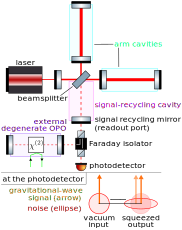
\includegraphics[angle=-90,width=0.9\textwidth]{nIS_config.pdf}
	\caption{\jam{(Purpose: explain configuration)} Nondegenerate internal squeezing configuration with all modes and losses labelled as explained in the text, compared to the mode diagram in Fig.~\ref{fig:nIS_mode_diagram}. The idler mode is not resonant in the arms and therefore the three modes are coupled as $\hat a$ to $\hat b$ to $\hat c$. The interferometer mirrors are labelled as the ETM (end test mass), ITM (input test mass), and SRM (signal-recycling mirror). The intra-cavity loss ports are shown as mirrors instead of beamsplitters, see Section~\ref{sec:optical_loss_background}, but the model of optical loss is the same. Compare the configuration to degenerate internal squeezing in Fig.~\ref{fig:dIS_config} and the nondegenerate OPO in Fig.~\ref{fig:nOPO_config}.}
	\label{fig:nIS_config}
\end{figure}

Nondegenerate internal squeezing consists of a nondegenerate squeezer placed inside the signal-recycling cavity of an interferometer, as shown in Figs.~\ref{fig:nIS_mode_diagram}~\ref{fig:nIS_config}. It is the same configuration as degenerate internal squeezing, shown in Fig.~\ref{fig:dIS_config}, except that the squeezer is operated nondegenerately, but it is better thought of as an all-optical alternative to stable optomechanical filtering, see Section~\ref{sec:modal_equivalence}. In the single-mode approximation, I consider the signal and idler modes resonant in the signal-recycling cavity, where the signal mode of the squeezer is at the carrier frequency $\omega_0$ and is resonant in the arms, while the idler mode at $\omega_0+\Delta$ is not resonant in the arms so that the arm and idler modes are not directly coupled, see Section~\ref{sec:modal_equivalence}. 
I model this configuration using the Hamiltonian method demonstrated several times in this thesis, and in particular, this model combines the nondegenerate OPO and degenerate internal squeezing models in Sections~\ref{sec:nOPO}~\ref{sec:dIS_model}, respectively. % There are no steps in this derivation that have not already appeared in this thesis \jam{(check this)}.
This model is based on and verified, in the lossless case, against Ref.~\cite{Li2020}. 
% \jam{(Probably need to talk about my methodology more -- state that this derivation presented is the last of a long line of increasing complexity (more losses, radiation pressure, pump phase, etc.) and that I have verified at each stage that the model recovers the previous model. This allowed me to also consider the impact of each subsequent addition in isolation. Moreover, I should re-emphasise that it reduces to the lossless case in Li and follows the same path as the verified models of dIS and the OPOs. The point is that this derivation is not controversial.)}
My methodology when constructing this model was to start with the lossless model in Ref.~\cite{Li2020} and progressively add each complication of optical loss in each mode, radiation pressure, and pump phase. At each stage of the progression, I verified that the model recovered the previous stage in the appropriate limits. This allowed me to study the effect of each complication separately rather than study the full model all at once. \jam{(need to be more critical of the approach?)} But, for brevity, I present the full model here.

Let the modes be labelled as shown in Fig.~\ref{fig:nIS_config}, which is as in Section~\ref{sec:dIS_model} but with the addition of $\hat c$ for the idler mode as in Section~\ref{sec:nOPO}. The Hamiltonian of this system is $\hat H = \hat H_0 + \hat H_I + \hat H_\gamma + \hat H_\text{GW}$ where~\cite{} \jam{(fill in Langevin Hamiltonian. change notation to distinguish $x$ and $\hat x$)}
\begin{align}
\hat H_0 &= \hbar \omega_0 \hat a^\dag \hat a + \hbar \omega_0 \hat b^\dag \hat b+ \hbar (\omega_0+\Delta) \hat c^\dag \hat c + \hbar (2\omega_0+\Delta) \hat u^\dag \hat u\\
\hat H_I &= i\hbar\omega_s(\hat a\hat b^\dag-\hat a^\dag\hat b) + \hbar \frac{x}{2} (e^{i\phi} \hat u \hat b^\dag \hat c^\dag+e^{-i\phi} \hat u^\dag \hat b \hat c) \\
\hat H_\gamma &= \int \ldots \\
\hat H_\text{GW} &= -\alpha (\hat{x}-L_\mathrm{arm}h(t))\left(\frac{\hat{a}+\hat{a}^\dag}{\sqrt{2}}\right)+\frac{1}{2\mu}\hat{p}^2.
\end{align}
As before, $\hat H_0$ describes the decoupled optical system, $\hat H_I$ describes the interaction between the three intra-cavity modes, $\hat H_\gamma$ describes the input/output coupling through the readout and loss ports listed below, and $\hat H_\text{GW}$ describes the coupling to the gravitational-wave signal and the evolution of the test mass mechanical mode.
There is vacuum entering the system intra-cavity to all three modes $\hat n^L_a, \hat n^L_b, \hat n^L_c$, at the readout port $\hat B_\text{in}, \hat C_\text{in}$, and in the detection chain $\hat n^L_\text{PD}$ which will be included later. Only the vacuum entering the readout port is present in the lossless model.
The Heisenberg-Langevin equations-of-motion for these operators can be found as before, using the bosonic and canonical commutation relations with all other commutators zero. I again (1) make the semi-classical and no-pump-depletion approximations to simplify the pump mode $\hat u\mapsto u=2\chi/x$, these approximations are valid below threshold, (2) enter the Interaction Picture to ignore $\hat H_0$, and (3) take fluctuating components of each operator but keep it implicit in the notation ($\delta\hat{Q}(t)\mapsto\hat{Q}$) because it does not change the equations-of-motion \jam{(is this true? it is not clear to me)}. I find the equations-of-motion to be
\begin{equation}\label{eq:nIS_EoM}
\begin{cases}
\dot{\hat{a}}=-\omega_s\hat{b} - \gamma_a \hat{a} + \sqrt{2\gamma_a}\hat{n}^L_a+\frac{i}{\hbar}\alpha(\hat{x}-L_\mathrm{arm}h)\frac{1}{\sqrt{2}}\\
\dot{\hat{b}}=\omega_s\hat{a} - i\chi e^{i\phi}\hat{c}^\dagger - \gamma^b_\mathrm{tot} \hat{b} + \sqrt{2\gamma^b_R}\hat{B}_\mathrm{in} + \sqrt{2\gamma_b}\hat{n}^L_b\\
\dot{\hat{c}}=-i\chi e^{i\phi}\hat{b}^\dagger - \gamma^c_\mathrm{tot} \hat{c} + \sqrt{2\gamma^c_R}\hat{C}_\mathrm{in} + \sqrt{2\gamma_c}\hat{n}^L_c\\
\dot{\hat{x}}=\frac{1}{\mu}\hat{p}\\
\dot{\hat{p}}=\alpha\left(\frac{\hat{a}+\hat{a}^\dag}{\sqrt{2}}\right).
\end{cases}
\end{equation}
I solve these equations in the Fourier domain. Let $\vec{\hat b}(\Omega)=[\hat b(\Omega), \hat b^\dag(-\Omega), \hat c(\Omega), \hat c^\dag(-\Omega)]^\text{T}$, where I use the compact notation $\tilde{\delta\hat{Q}}(\Omega)\mapsto\hat{Q}(\Omega)$, with similar signal-idler vectorisation for each signal and idler mode as in Section~\ref{sec:nOPO} and $\vec h(\Omega)=\tilde h(\Omega) [1,1,0,0]^\text{T},\quad \vec{\hat a}(\Omega)=[\hat a(\Omega), \hat a^\dag(-\Omega),0,0]^\text{T}$ and similarly for $\vec{\hat n}^L_a(\Omega)$.
\jam{(Show more working here? See cut derivation in appendix.)}
Solving the resulting algebraic equations, I find that
\begin{align}
\mathrm{M}_b\vec{\hat{b}}(\Omega)&= \omega_s\begin{bsmallmatrix}
1 &  &  &  \\
 & 1 &  &  \\
 &  & 0 &  \\
 &  &  & 0
\end{bsmallmatrix}\mathrm{M}_a^{-1}\left(\sqrt{2\gamma_a}\begin{bsmallmatrix}
1 &  &  &  \\
 & 1 &  &  \\
 &  & 0 &  \\
 &  &  & 0
\end{bsmallmatrix}\vec{\hat{n}}^L_a(\Omega)-i\beta\begin{bsmallmatrix}
1 &  &  &  \\
 & -1 &  &  \\
 &  & 0 &  \\
 &  &  & 0
\end{bsmallmatrix}\vec{h}(\Omega)\right)\\&+ \sqrt{2}\begin{bsmallmatrix}
\sqrt{\gamma^b_R} &  &  &  \\
 & \sqrt{\gamma^b_R} &  &  \\
 &  & \sqrt{\gamma^c_R} &  \\
 &  &  & \sqrt{\gamma^c_R}
\end{bsmallmatrix}\vec{\hat B}_\mathrm{in}(\Omega) + \sqrt{2}\begin{bsmallmatrix}
\sqrt{\gamma_b} &  &  &  \\
 & \sqrt{\gamma_b} &  &  \\
 &  & \sqrt{\gamma_c} &  \\
 &  &  & \sqrt{\gamma_c}
\end{bsmallmatrix}\vec{\hat n}^L_b(\Omega)\\
\mathrm{M}_a &= (\gamma_a-i\Omega)\mathrm{I}+\frac{i\rho}{\Omega^2 \sqrt{2}}\begin{bsmallmatrix}
1 & 1 &  &  \\
-1 & -1 &  &  \\
 &  & 0 &  \\
 &  &  & 0
\end{bsmallmatrix}\\
\text{M}_b&=\begin{bsmallmatrix}
\gamma^b_\mathrm{tot} &  &  &  \\
 & \gamma^b_\mathrm{tot} &  &  \\
 &  & \gamma^c_\mathrm{tot} &  \\
 &  &  & \gamma^c_\mathrm{tot} 
\end{bsmallmatrix}-i\Omega \text{I}+\chi \begin{bsmallmatrix}
0 &  &  & i e^{i\phi} \\
 & 0 & -i e^{-i\phi} &  \\
 & i e^{i\phi} & 0 &  \\
-i e^{-i\phi} &  &  & 0
\end{bsmallmatrix}+\omega_s^2\begin{bsmallmatrix}
1 &  &  &  \\
 & 1 &  &  \\
 &  & 0 &  \\
 &  &  & 0
\end{bsmallmatrix}\text{M}_a^{-1}\begin{bsmallmatrix}
1 &  &  &  \\
 & 1 &  &  \\
 &  & 0 &  \\
 &  &  & 0
\end{bsmallmatrix}.
\end{align}
Where $\beta, \rho$ are given by Eq.~\ref{eq:beta_and_rho}, $\text{I}$ is the 4 by 4 identity matrix, and all off-diagonal terms in each matrix are zero unless otherwise shown \jam{(is this clear or would it be better to include them explicitly?)}. Using $\Gamma= \frac{1}{\sqrt2}\begin{bsmallmatrix}
1 & 1 &  &  \\
-i & i &  &  \\
 &  & 1 & 1 \\
 &  & -i & i
\end{bsmallmatrix}$ and the input/output relations at the readout port and the detection loss port given by Eq.~\ref{eq:nOPO_IO_relations}, I find the signal and idler quadratures~\footnote{Where $\vec{\hat X}(\Omega)=[\hat X_{b,1}(\Omega),\hat X_{b,2}(\Omega),\hat X_{c,1}(\Omega),\hat X_{c,2}(\Omega)]^\text{T}$, as in Section~\ref{sec:nOPO}.} at the photodetector to be
\begingroup
\allowdisplaybreaks
\begin{align}\label{eq:nIS_Xpd}
\vec{\hat X}_\mathrm{PD}(\Omega)&=\text{T}\vec h(\Omega)+\text{R}_\text{in}\vec{\hat X}_\mathrm{in}(\Omega)+\text{R}^L_a\vec{\hat X}^L_a(\Omega)+\text{R}^L_b\vec{\hat X}^L_b(\Omega)+\text{R}^L_\text{PD}\vec{\hat X}^L_\text{PD}(\Omega)\\
\text{T}&=-\sqrt{1-R_\text{PD}}\omega_s(-i\beta)\Gamma \sqrt{2}\begin{bsmallmatrix}
\sqrt{\gamma^b_R} &  &  &  \\
 & \sqrt{\gamma^b_R} &  &  \\
 &  & \sqrt{\gamma^c_R} &  \\
 &  &  & \sqrt{\gamma^c_R}
\end{bsmallmatrix}\text{M}_b^{-1}\begin{bsmallmatrix}
1 &  &  &  \\
 & 1 &  &  \\
 &  & 0 &  \\
 &  &  & 0
\end{bsmallmatrix}\text{M}_a^{-1}\begin{bsmallmatrix}
1 &  &  &  \\
 & -1 &  &  \\
 &  & 0 &  \\
 &  &  & 0
\end{bsmallmatrix}\\
\text{R}_\text{in}&=\sqrt{1-R_\text{PD}}\Gamma\left(\text{I}-2\begin{bsmallmatrix}
\sqrt{\gamma^b_R} &  &  &  \\
 & \sqrt{\gamma^b_R} &  &  \\
 &  & \sqrt{\gamma^c_R} &  \\
 &  &  & \sqrt{\gamma^c_R}
\end{bsmallmatrix}\text{M}_b^{-1}\begin{bsmallmatrix}
\sqrt{\gamma^b_R} &  &  &  \\
 & \sqrt{\gamma^b_R} &  &  \\
 &  & \sqrt{\gamma^c_R} &  \\
 &  &  & \sqrt{\gamma^c_R}
\end{bsmallmatrix}\right)\Gamma^{-1}\\
\text{R}^L_a&=-\sqrt{1-R_\text{PD}}\omega_s\Gamma 2\sqrt{\gamma_a}\begin{bsmallmatrix}
\sqrt{\gamma^b_R} &  &  &  \\
 & \sqrt{\gamma^b_R} &  &  \\
 &  & \sqrt{\gamma^c_R} &  \\
 &  &  & \sqrt{\gamma^c_R}
\end{bsmallmatrix}\text{M}_b^{-1}\begin{bsmallmatrix}
1 &  &  &  \\
 & 1 &  &  \\
 &  & 0 &  \\
 &  &  & 0
\end{bsmallmatrix}\text{M}_a^{-1}\begin{bsmallmatrix}
1 &  &  &  \\
 & 1 &  &  \\
 &  & 0 &  \\
 &  &  & 0
\end{bsmallmatrix}\Gamma^{-1}\\
\text{R}^L_b&=-\sqrt{1-R_\text{PD}}\Gamma 2\begin{bsmallmatrix}
\sqrt{\gamma^b_R} &  &  &  \\
 & \sqrt{\gamma^b_R} &  &  \\
 &  & \sqrt{\gamma^c_R} &  \\
 &  &  & \sqrt{\gamma^c_R}
\end{bsmallmatrix}\text{M}_b^{-1}\begin{bsmallmatrix}
\sqrt{\gamma^b_R} &  &  &  \\
 & \sqrt{\gamma^b_R} &  &  \\
 &  & \sqrt{\gamma^c_R} &  \\
 &  &  & \sqrt{\gamma^c_R}
\end{bsmallmatrix}\Gamma^{-1}\\
\text{R}^L_\text{PD}&=\sqrt{R_\text{PD}} \text{I}.
\end{align}
\endgroup
The total quantum noise is given by the spectral density matrix Eq.~\ref{eq:total_noise_matrix}, which simplifies, assuming uncorrelated vacuum at each loss port, to
\begin{equation}\label{eq:nIS_Sx}
\text{S}_X=\text{R}_\text{in}\text{R}_\text{in}^\dag+\text{R}^L_a{\text{R}^L_a}^\dag+\text{R}^L_b{\text{R}^L_b}^\dag+\text{R}^L_\text{PD}{\text{R}^L_\text{PD}}^\dag.
\end{equation} % same expression as dIS
Which is divided into 2 by 2 blocks of signal-signal, signal-idler, and idler-idler (co)variances as in Section~\ref{sec:nOPO} \jam{(are the signal-signal and idler-idler covariances all zero? how many freedoms remaining in the signal-idler covariances?)}. The pump phase only appears in the off-diagonal, signal-idler blocks.
The vector of signal transfer functions, with respect to $\tilde h(\Omega)$, to each signal and idler quadrature at the photodetector is
\begin{equation}\label{eq:nIS_sigRO_signal_response}
\text{T}\begin{bsmallmatrix}1 \\1\\0\\0\end{bsmallmatrix} = \frac{2 \beta \sqrt{1-R_\text{PD}} \omega_s}{(\gamma_a-i \Omega ) \left(\chi ^2-(\gamma^b_\text{tot}-i\Omega) (\gamma^c_\text{tot}-i\Omega)\right)-\omega_s^2 (\gamma^c_\text{tot}-i \Omega )} \begin{bsmallmatrix}0 \\-\sqrt{\gamma^b_R}(\gamma^c_\text{tot}-i\Omega)\\\sqrt{\gamma^c_R}\chi\cos(\phi)\\\sqrt{\gamma^c_R}\chi\sin(\phi)\end{bsmallmatrix}.
\end{equation}
Therefore, there is gravitational-wave signal in the second signal quadrature and each idler quadrature. For simplicity and to compare to Ref.~\cite{Li2020}, here I will consider measuring the second signal quadrature which I will refer to as signal readout, henceforth. However, this is not necessarily the optimum readout of the signal quadratures since the noise might be sufficiently lower in the first quadrature to preference a combined measurement. I will consider this and other readout schemes, such as measurements of the idler quadratures and combinations of the signal and idler quadratures, in Chapter~\ref{chp:idler_readout}.
Therefore, the quantum noise and signal responses of the signal readout scheme are, respectively, $\sqrt{(\text{S}_X)_{2,2}}$ and $\abs{\left(\text{T}\begin{bsmallmatrix}1 \\1\\0\\0\end{bsmallmatrix}\right)_2}$, and the sensitivity, quoted as the noise-to-signal ratio \jam{(check that this sqrt form is consistent with the background chapters and the literature)}, is
\begin{equation}\label{eq:nIS_sigRO_sens}
\sqrt{S_h} = \frac{\sqrt{(\text{S}_X)_{2,2}}}{\abs{\left(\text{T}\begin{bsmallmatrix}1 \\1\\0\\0\end{bsmallmatrix}\right)_2}}.
\end{equation}
% verified these results by repeating the model with 2x2 matrices and 4x4 matrices, important to mention this because it is part of the methodology
\jam{(Include full expression in an appendix?)} I have partially verified this result by repeating the derivation using 2 by 2 matrices~\footnote{Which is not a physically meaningful difference, but it separates the signal and idler such that the derivations are not identical.}, and will compare it to known limits below. %in Section~\ref{sec:nOPO_reduction}.


\section{Results}
\label{sec:nIS_sigRO_results}

\jam{(Are these results quantitative enough?)}

\jam{(Update after restructuring order of results)}
I will now examine some of the immediate results of the model: (1) the general features of the signal and noise responses and sensitivity, (2) the reduction to known models in certain loss limits, and (3) the stability of the system.
\jam{(link to parameter set used)}

\subsection{General behaviour}
\label{sec:nIS_general_behaviour}
% should this be down in results section? --> this is a results chapter, maybe include a short section discussing the general performance (separate from the science case analysis in chapter 5?)

% plot: classic N, S, NSR; also noise budget plot
% need to show some example plots here to set up those in the next section?
\begin{figure}
	\centering
	\includegraphics[width=\textwidth]{nIS_N_S_NSR.pdf}
	\caption{\jam{(Purpose: Plain plot to discuss the general features of nIS)} \jam{(Examine lossless plot first instead?)} Nondegenerate internal squeezing signal readout with all losses included, showing the quantum noise response (top panel), signal response (middle panel), and sensitivity (bottom panel). The effect of the squeezer and the radiation pressure noise (turned off by setting $\rho=0$) on the sensitivity is understood by examining the signal and noise separately. The slope of the radiation pressure noise with the squeezer on changes around 10~Hz which is an effect of losses, and the same effect causes the signal to not be amplified down to DC. The squeezer parameter is normalised to threshold which will be found later.}
	\label{fig:nIS_general_sens}
\end{figure}

\jam{(should I show the lossless limit first?)}

% analyse typical nIS plot features before getting into different tests
The sensitivity of nondegenerate internal squeezing is shown in Fig.~\ref{fig:nIS_general_sens} \jam{(for what parameters?)}. I examine the signal and noise responses separately to understand the origin of the features in the sensitivity curve.
With the squeezer off, the sensitivity curve is shaped by the radiation-pressure noise below 10~Hz and the signal response resonance at the sloshing frequency 5~kHz with bandwidth 500~Hz determined by the signal readout rate $\gamma^b_R$, as discussed in Section~\ref{sec:dIS_results}. With the squeezer turned on, (1) the shot noise is anti-squeezed around a frequency determined by the squeezer parameter, sloshing frequency, and loss rates; (2) the radiation-pressure noise worsens to now dominate below 100~Hz; and (3) the signal is amplified around the same frequency as the shot noise and at frequencies down to 10~Hz, below which it converges to the value without squeezing due to losses. These changes mean that the squeezer improves the sensitivity from 40--4000~Hz and worsens it outside that band except above 10~kHz where the sensitivity converges to the value without squeezing.
These quoted frequencies are specific to this parameter set but the general performance is the same: nondegenerate internal squeezing leads to improved sensitivity at some broad range of ``middle'' frequencies at the cost of ``low'' frequency sensitivity. 
Some of these effects will be explained later, e.g.\ the frequency around which the shot noise and the signal peak are amplified is determined by the threshold of the system, but some of these results can be explained immediately.
 % and the effect of losses will be left until I consider gravitational-wave detection feasibility.
% changing the signal response via the white-light cavity effect?
% why aren't the changes local to the sloshing frequency, like dIS?
The signal response is amplified by analogy to the filter (white-light) cavity effect of the optomechanical analogue, the resonance of the coupled cavity system is changed by introducing the idler mode \jam{(is this true? I am not sure. the signal response still falls off at the same rate so bandwidth doesn't seem to improve except by the LF amplification?)}. The change in the resonance behaviour from a two-mode to a three-mode coupled system means that the changes are not localised to the sloshing frequency, unlike degenerate internal squeezing in Section~\ref{sec:dIS_results} \jam{(check this, shouldn't this mean that they are still expected around the coupling frequencies?)}. 
%In the simple explanation of the signal-recycling cavity reflecting the light back into the arms to experience the gravitational wave more, the addition of the idler mode, which is not directly coupled to the arms or measured, somehow \jam{(how/why? this is wishy-washy)}.
% why does radiation pressure noise worsen?
% ~\footnote{I only talk about the radiation pressure noise where it is dominant, i.e.\ at ``low'' frequencies below the Standard Quantum Limit \jam{(is this necessary to say?)}}
Therefore, the radiation pressure noise at ``low'' frequencies can be affected and is also anti-squeezed. \jam{(why is it amplified, happens in lossless case as well? why does the other quadrature appear now? is it worsened proportionally to the pump power?)}

% To understand how the radiation pressure noise is affected, I consider how it appears in each of the contributions to the total quantum noise, shown in Fig.~\ref{fig:nIS_sigRO_noise_budget}. The radiation pressure noise appears in the contribution from the readout port and each intra-cavity loss port because these noises are coupled indirectly to the arm mode, unlike the detection loss which therefore has only shot noise. In particular, opening the idler readout port introduces more vacuum and turning the squeezer on indirectly couples the idler mode and this noise into the signal readout, which is why radiation pressure noise worsens by turning the squeezer on even when there are no losses \jam{(check this)}, which will be shown later in Fig.~\ref{fig:nIS_lossless}. \jam{(why is the shot noise not amplified at LF?)}
% This is because the radiation pressure noise, with the gravitational-wave signal, enters the measured, second signal quadrature after the input test mass. Having already seen the arm cavity loss, it gets added here to each of the noises that travel through the signal mode \jam{(what am I trying to say?)}. It is then anti-squeezed \jam{(check this)} and read out.

% explain the effect of each parameter? (except leave tolerance to losses to science case chapter)
% in terms of the configuration parameters rather than derived parameters such as the sloshing frequency and readout rates
\jam{(Is this paragraph necessary? true? complete?)}
The effect of each configuration parameter is similar to the effect on the interferometer without squeezing in Sections~\ref{sec:intro_IFO}~\ref{sec:dIS_results}. To summarise, increasing the circulating power in the arms increases the sensitivity at all frequencies. Increasing the arm length increases the same scalar factor $\beta$ as the power but also reduces the free-spectral range of the signal response (i.e.\ the signal response falls off at a lower frequency) and decreases the sloshing (peak) frequency. The sloshing frequency also decreases with decreased input test mass transmission and longer signal-recycling cavities. Increasing the signal-recycling length decreases the bandwidth of the signal peak \jam{(Are there two bandwidths? The FSR of the arms sets where the signal falls off and the readout rate sets the smaller bandwidth around the sloshing frequency peak? If so, then clarify.)}, which is also decreased by decreased signal-recycling mirror transmission. The radiation-pressure noise increases with heavier test masses and increased pump power. Finally, increased pump power also increases the peak shot noise and signal amplification, and the pump phase does not affect signal readout. \jam{(I am claiming a lot here without figures or citations, what to include?)}


\subsection{Reduction to known systems}

% show that this follows from the EoM but can be verified by looking at the plots
To partially verify the model, I show that it reduces to the expected limits when (1) the losses are removed and (2) the arm loss is taken to infinity. I predict the behaviour by taking the limits of the equations-of-motion in Eq.~\ref{eq:nIS_EoM} and verify it by examining the plots of the noise and signal responses.

\subsubsection{Lossless limit}
\label{sec:nIS_lossless_limit}

\begin{figure}
	\centering
	\includegraphics[width=\textwidth]{nIS_lossless.pdf}
	\caption{\jam{(Purpose: show limits 1/2)} \jam{(Add noise and signal back in and show before lossy result?)} Nondegenerate internal squeezing sensitivity in the lossless limit, with and without radiation pressure noise, compared to the lossless optomechanical analogue from Section~\ref{sec:sWLC}. This is shown for 500~Hz signal readout rate and no idler readout rate \jam{(check)}. The sensitivity converges as shown, as do the signal and noise responses. Compared to the lossy sensitivity without radiation-pressure noise in Fig.~\ref{fig:nIS_general_sens}, the signal DC response is improved which means that the losses determine the bandwidth of the squeezer's signal amplification \jam{(check)}. \jam{(mention that the noise is not anti-squeezed)} }
	\label{fig:nIS_lossless}
\end{figure}

In the lossless limit, $\gamma_a=\gamma_b=\gamma_c=R_\text{PD}=0$, with the idler readout rate turned off, $\gamma^c_R=0$, the equations-of-motion of nondegenerate internal squeezing in Eq.~\ref{eq:nIS_EoM} reduce to those of the lossless optomechanical analogue in Ref.~\cite{Li2020}. The resulting sensitivity also reduces to the same limit, as shown in Fig.~\ref{fig:nIS_lossless}. This behaviour is expected from the comparison of the mode structure of the two lossless systems, see Section~\ref{sec:modal_equivalence}.
% this is because of the use of alpha from Li and not Korobko
I will compare the two lossy systems in the next chapter. 
% no losses means no antisqueezing of shot noise but yes RPN, why? threshold=0 problem?
Without losses, the shot noise is not anti-squeezed and the signal amplification persists down to DC. Since the idler readout rate is zero and there is no loss, the threshold is poorly defined because there is no mechanism for light to leave the idler mode, which will be discussed later. However, taking the limit of smaller and smaller losses shows that the shot noise peak decreases for fixed pump power below threshold \jam{(check this, why?)}. The bandwidth of the signal amplification is determined by the losses present and therefore the DC improvement is lost when losses are added and the bandwidth no longer extends to DC \jam{(check. why? compare lossless and lossy plots directly)}.


\subsubsection{High arm loss limit}
\label{sec:nOPO_reduction}

% \begin{figure}
% 	\centering
% 	\includegraphics[width=\textwidth]{nIS_nOPO_limit.pdf}
% 	\caption{\jam{(Purpose: show limits 2/2)} \jam{(Can cut this plot and instead just claim the limit in the text.)} Nondegenerate internal squeezing shot noise response showing the high arm loss limit compared to the response from a nondegenerate OPO with the input test mass fully reflective. The signal and idler readout rates are assumed symmetric. The shot noise converges as expected.}
% 	\label{fig:nIS_signal_nOPO_limit}
% \end{figure}

% full 4x4 matrix agrees, not just variance 1,1
% give best explanation of ITM T=0, but can admit that while the maths is clear the physics is not obvious -- potentially requires more thought
In the high arm loss limit, $\gamma_a\rightarrow\infty$, the equations-of-motion of nondegenerate internal squeezing in Eq.~\ref{eq:nIS_EoM} reduce to those in Eq.~\ref{eq:nOPO_EoM} for a nondegenerate OPO between the signal-recycling mirror and a fully-reflective input test mass.
I verify this limit by checking the shot noise matrix $\text{S}_X|_{\rho=0}$ and showing that each of its terms also converge. \jam{(just shot noise? check if the RPN vanishes)}
This is similar to how the shot noise of degenerate internal squeezing converges to that of a degenerate OPO with the input test mass fully reflective, see Section~\ref{sec:dIS_optical_loss}, where the explanation for why the mirror is fully reflective is the same as that case. 

% therefore mystery of the idler loss carries over: idler loss cannot be zero
Therefore, for a given set of losses, nondegenerate internal squeezing exists somewhere between the lossless optomechanical analogue and the nondegenerate OPO. And so, I expect features to be inherited from these limiting configurations, such as how the fact that threshold is poorly defined when idler loss is zero is inherited from the nondegenerate OPO.


\section{Stability and threshold}

I will now consider the stability and threshold of nondegenerate internal squeezing to determine for what parameters it is stable and below threshold, which is required for experiments. I will use the no-pump-depletion assumption to link when the system is marginally stable and when it is at threshold.

\subsection{Stability}
\label{sec:nIS_stability}

% plot: imaginary part of poles
\begin{figure}
    \centering
    \includegraphics[width=0.8\textwidth]{nIS_stability.pdf}
    \caption{\jam{(Purpose: show stability)} \jam{(Supervisors once requested Nyquist plots, is this sufficient?)} Stability of nondegenerate internal squeezing, for lossless (top panel) and lossy (bottom panel) cases. Showing the imaginary part of the poles of the transfer functions; where the imaginary part becomes positive the system becomes unstable~\cite{}. The different colours indicate different numerical solutions for the zeroes of the common denominator. The denominator does not depend on detection loss $R_\text{PD}$, as shown in Eq.~\ref{eq:nIS_sigRO_signal_response}. Singularity threshold will be defined such that the system is stable below threshold, and therefore the value of $\chi_\text{thr}$ is different between the two panels.}
    \label{fig:nIS_stability}
\end{figure}

Stability is a feature of nondegenerate internal squeezing that might not be fully inherited from its limiting configurations. I use the same method to determine stability as Section~\ref{sec:dIS_results}. Like degenerate internal squeezing, the signal and noise transfer functions are rational functions of $\Omega, \chi$ with denominators~\footnote{I state these for the modulus-squared transfer functions, i.e.\ $(\text{S}_X)_{2,2}$ and $\abs{\left(\text{T}\begin{bsmallmatrix}1 \\1\\0\\0\end{bsmallmatrix}\right)_2}^2$, but the poles, i.e.\ zeros of $q$, do not change under the square root.} given by $q(\Omega,\chi)$ and $\Omega^4 q(\Omega,\chi) q(\Omega,-\chi)$, respectively, except that here $q$ only depends on $\chi^2$ and so the noise transfer function denominator is $\Omega^4 q(\Omega,\chi)^2$, where $q$ is some polynomial in $\Omega, \chi$, 
\begin{align}\label{eq:nIS_denom}
q(\Omega,\chi)&=\left(\gamma_a^2+\Omega ^2\right) \left(\Omega ^2 \left({\gamma^b_\text{tot}}^2+{\gamma^c_\text{tot}}^2+2 \chi ^2\right)+\left({\gamma^b_\text{tot}} {\gamma^c_\text{tot}}-\chi ^2\right)^2+\Omega ^4\right)\\
&-2 \omega_s^2 \left(\gamma_a {\gamma^c_\text{tot}} \chi ^2-\gamma_a {\gamma^b_\text{tot}} \left({\gamma^c_\text{tot}}^2+\Omega ^2\right)+\Omega ^2 \left({\gamma^c_\text{tot}}^2+\chi ^2+\Omega ^2\right)\right)+\omega_s^4 \left({\gamma^c_\text{tot}}^2+\Omega ^2\right).
\end{align}
This means that the zeros of the transfer functions are the shared zeros of $q$, except for the radiation-pressure noise singularity at $\Omega=0$ which I ignore because it comes from the horizontally free-falling mass assumption and physically the resonance of the test mass is finite~\cite{}. That the rest of the poles are shared is expected because the stability of the system should be the same for the signal and noise \jam{(should it?)}~\cite{}.
Therefore, nondegenerate internal squeezing is unstable if any of the complex $\Omega$ zeros of $q$ have a positive imaginary part and is marginally stable if any of them have no imaginary part. As shown in Fig.~\ref{fig:nIS_stability}, the lossless system is stable for all $\chi\leq\omega_s$ which agrees with Ref.~\ref{Li2020}. The lossy system is also stable up to a certain point that I will shortly define to be the lossy threshold. Because the no-pump-depletion assumption breaks above threshold, the behaviour there cannot be inferred from Fig.~\ref{fig:nIS_stability}.
% non-effect of RP, pump phase
Since Eq.~\ref{eq:nIS_denom} only depends on the pump power, readout and loss rates, and sloshing frequency, therefore, other factors, such as radiation pressure or pump phase, do not affect the zeros of $q$ or the stability.

\jam{(need to worry about MIMO? see Li2021)}

\subsection{Singularity threshold}
\label{sec:singularity_threshold}
% motivate this by the previous section's looking at poles, now looking at real poles that could be encountered, to avoid confusion with the complex poles that are always present I will call these real poles ``singularities''

% \jam{(Rewrite the following as the threshold of stability, should just be one paragraph, make clear that the link to gain-loss balancing is just that if there is a net gain but no pump depletion then energy is demonstrably unpreserved and the field will grow without end which is unstable. But be honest that I do not know and that this result would be different with pump-depletion added.)}

\begin{figure}
    \centering
    \includegraphics[width=\textwidth]{nIS_on_threshold.pdf}
    \caption{\jam{(Purpose: show that singularity threshold actually gives singularities. Is this necessary? Could just cut this plot and claim that I can observe the singularity when plotting in the text?)} Nondegenerate internal squeezing noise, signal, and sensitivity when approaching and at threshold. At threshold, the no-pump-depletion assumption breaks and the transfer functions are singular. The peaks in the noise and signal responses are finite and a false peak in the sensitivity appears at the threshold frequency because of numerical error and limited sample points \jam{(check this, clarify what should be there instead, study limiting behaviour where singularities cancel. Could just cut the plot to not deal with this.)}. For the threshold behaviour of the other configurations in this thesis see Figs.~\ref{fig:dOPO_variances}~\ref{fig:nOPO_variances}~\ref{fig:dIS_sensitivity}.}
    \label{fig:nIS_on_threshold}
\end{figure}

\jam{(Can shorten this section. Weave-in stability more.)}

% \jam{(Emphasise that this is original work and that it is a clever approach.)}
Finding the threshold of nondegenerate internal squeezing is required to understand where this model is valid and, experimentally, how high the pump power can be raised without lasing.
The threshold of lossy degenerate and nondegenerate internal squeezing is not available in the literature \jam{(check this)}, and in this section, I present my method for determining threshold in these models. %, which uses the no-pump-depletion assumption.
As established in Sections~\ref{sec:dOPO_threshold}~\ref{sec:nOPO_results}~\ref{sec:dIS_results}, the threshold of a squeezing system is the boundary where gains balance losses and the no-pump-depletion assumption breaks. If pump depletion is included, then beyond threshold the system begins lasing as the cavity field is (finitely) coherently amplified~\cite{} and energy is taken from the pump mode. Since I assume no pump depletion, beyond threshold, the net gain at the squeezer instead leads to unbounded, coherent amplification of the cavity mode~\cite{lasingMaterial}, and therefore the system becomes unstable \jam{(is this clear?)}. Therefore, my method is to define threshold as the point of marginal stability of the system with the no-pump-depletion assumption and assume that whenever the system becomes unstable it is because of the squeezer reaching threshold \jam{(justify this assumption)}.

Formally, my method is to define the ``singularity threshold''~\footnote{Which, perhaps, might be better called the ``stability threshold''.} as the smallest non-negative~\footnote{Because pump phase is included explicitly in the models, the squeezer parameter is non-negative.} value of the squeezing parameter such that the anti-squeezed quadrature of the quantum noise has a singularity at some (real) frequency. In particular, I look for points where the anti-squeezed quadrature, i.e.\ any of the diagonal terms of $\text{S}_X$, diverges to infinity in $(\Omega,\chi)\subset\mathbb{R}^2$ space~\footnote{To reduce confusion, I do not call these points poles since, unlike when considering stability, I am restricting $\Omega$ to be real and so the transfer function is not defined on $\mathbb{C}$.}. %Since I include the pump phase in my models, $\chi$ is further restricted to be positive.  \jam{(Check this: looking at the imaginary part of the poles for stability and looking for real poles (i.e. poles on the real axis) for threshold are the same solutions, surely?)}
Defining threshold with respect to anti-squeezing is better than squeezing because the singularities of the anti-squeezed quadrature are expected to be robust to losses, unlike the zeros of the squeezed quadrature, as shown in Fig.~\ref{fig:dOPO_variances}. 
I find the (real~\footnote{The reality condition is used to simplify the zeros of $q$, as in the solution for $\chi^2$ there is an imaginary component that, when set to zero, gives the real $\Omega$ solution.}) singularities of the noise transfer function (squared) $S_X$, i.e.\ the zeros of its denominator, for each squeezing configuration in this thesis to be at \jam{(check that $\gamma_c\mapsto\gamma^c_\text{tot}$)}
\begingroup
\allowdisplaybreaks
\begin{align}\label{eq:singularity_threshold}
\text{degenerate OPO}&: \Omega_\text{thr}=0, \chi_\text{thr}=\gamma^b_\mathrm{tot}\\
\text{nondegenerate OPO}&: \Omega_\text{thr}=0, \chi_\text{thr}=\sqrt{\gamma^b_\mathrm{tot}\gamma^c_\text{tot}}\\
\text{degenerate internal squeezing}&:\begin{cases}
\Omega_1=0, \chi_1=\gamma^b_\mathrm{tot}+\frac{\omega_s^2}{\gamma_a};&\gamma_a\neq0\\
\Omega_2=\sqrt{\omega_s^2-\gamma_a^2}, \chi_2=\gamma^b_\mathrm{tot}+\gamma_a;&\omega_s\geq\gamma_a\geq0
\end{cases}\\
\text{nondegenerate internal squeezing}&:\nonumber\\&\hspace{-5cm}\begin{cases}
\Omega_1=0, \chi_1=\sqrt{\gamma^c_\text{tot}(\gamma^b_\mathrm{tot}+\frac{\omega_s^2}{\gamma_a})};&\gamma^c_\text{tot}\neq0,\gamma_a\neq0\\
\Omega_2=\sqrt{\frac{\gamma^c_\text{tot}\omega_s^2-\gamma_a(\omega_s^2+\gamma_a(\gamma^b_\mathrm{tot}+\gamma^c_\text{tot}))}{\gamma^b_\mathrm{tot}+\gamma^c_\text{tot}}}, \chi_2=\sqrt{(\gamma_a+\gamma^b_\mathrm{tot})(\gamma_a+\gamma^c_\text{tot}+\frac{\omega_s^2}{\gamma^b_\mathrm{tot}+\gamma^c_\text{tot}})};&\gamma^c_\text{tot}\neq0,(*)
\end{cases}\nonumber\\
(*)&:\gamma^c_\text{tot}\omega_s^2\geq\gamma_a\left(\omega_s^2+\gamma_a(\gamma^b_\mathrm{tot}+\gamma^c_\text{tot})\right)
\end{align}
\endgroup
% frequency around which shot noise and signal are amplified in fig:nIS_general_sens is determined (but not exactly) the threshold frequency
% which pole is chosen tells us the closeness to nOPO or lossless sWLC
I have verified these values by plotting the noise transfer function and observing the singularity, e.g.\ as shown in Fig.~\ref{fig:nIS_on_threshold}. For squeezer parameter near threshold, e.g.\ $\chi=0.95\chi_\text{thr}$ in Fig.~\ref{fig:nIS_general_sens}, the peak frequency around which the shot noise and signal are amplified is determined by the threshold frequency~\footnote{Consider this peak as a slice with constant $\chi$ of the region around the singularity in (real) $(\Omega,\chi)$ space.}. When multiple singularities are listed above, the singularity threshold is determined by the smallest $\chi$ value:
\begin{equation}
\chi_\text{thr}=\min_{i\in\{1,2\}}(\chi_i),\quad\Omega_\text{thr}=\Omega_{\underset{i\in\{1,2\}}{\text{argmin}}(\chi_i)}.
\end{equation}
Which singularity has the smallest squeezer parameter changes as the losses change, and where it changes, the singularities merge by inspection~\footnote{Therefore, singularity threshold is continuous for these configurations.}. The smallest squeezer parameter gives the first singularity hit when increasing the pump power from zero. The merging of the singularities could also be used, perhaps, to indicate when the lossy configuration's behaviour becomes closer to the OPO limit than to the lossless configuration.
% $\Omega^4$ factor in RP denominator is the resonance, but is unrelated to the squeezer
% pump phase does not change threshold either
Singularity threshold is not affected by radiation pressure or pump phase since they do not affect the zeros of the denominator $q$ of the noise transfer function, as explained in Section~\ref{sec:nIS_stability}. Physically, the pump phase is irrelevant because the singularity threshold looks at the anti-squeezed quadrature wherever it lies in the quadrature basis \jam{(physical reason why the RPN does not matter?)}.
% Although the radiation pressure does introduce (1) a zero at $\Omega=0$ and (2) a factor $q(\Omega,-\chi)$, these can be ignored because, respectively, (1) comes from the free-falling mass assumption which is only valid at frequencies above the actual test mass resonance and therefore the physical behaviour will not have this singularity and (2) only increases the multiplicity of the zeros because the result is independent of pump phase and therefore of the sign of $\chi$. 

To explain how I first devised this method, which was separate from considering stability, since lossless degenerate internal squeezing on threshold has a minimum squeezed quadrature of zero, I initially tried to maximise the anti-squeezed quadrature of lossy nondegenerate internal squeezing against $(\Omega,\chi)$. But doing so numerically encountered division-by-zero errors which lead me to examine the transfer functions and find the singularities, i.e.\ the real zeros of $q$, analytically. The key insights were then realising that both the OPOs have singularities at $\Omega=0$ in the anti-squeezed quadrature on threshold and that a pole on the real axis corresponds to marginal stability.

\begin{figure}
    \centering
    \includegraphics[width=\textwidth]{nIS_threshold.pdf}
    \caption{\jam{(Purpose: show evolution and limits of threshold. Is this simplified enough?)} Nondegenerate internal squeezing trajectories of singularities of the anti-squeezed noise in $(\Omega, \chi)$ space as losses are changed. The idler readout rate and the signal loss are zero. There are two loss effects shown: (1) the idler loss is changed and the arm loss is zero along the red line and (2) the idler loss is fixed and non-zero and the arm loss is changed along the cyan and blue lines. 
    The path from the lossless to the high arm loss limit should be read from point (a) with all losses zero to point (b) along the red line with idler loss $T_{l,c}=0.1$, then changing arm loss to point (c) along the cyan line with $T_{l,a}\approx0.3,\;T_{l,c}=0.1$, and, finally, to point (d) along the blue line with $T_{l,a}=1,\;T_{l,c}=0.1$. The blue line shown does not reach point (d) because of limited numerical sampling.
    The idler loss is large, $T_{l,c}=0.1$, to show the trajectories more clearly, when it is realistic, e.g.\ $T_{l,c}=1000\text{ppm}$ the singularities collide closer to $\chi=\omega_s$ \jam{(check position of (b) as well)}. The second singularity when the arm loss is zero is at infinity. \jam{(is the explanation in the text sufficient?)}}
    \label{fig:nIS_threshold_traj}
\end{figure}

Singularity threshold in Eq.~\ref{eq:singularity_threshold} recovers the known threshold values for the OPOs from Sections~\ref{sec:dOPO_threshold}~\ref{sec:nOPO_results}. Although it also recovers the threshold for degenerate internal squeezing from Section~\ref{sec:dIS_results}, it does not necessarily find the minimum of the squeezed quadrature, which I discuss in Appendix~\ref{app:dIS_singularity_thr}.
\jam{(Does it agree with existing stability analysis?)}
% this resolves the mystery of idler loss --> means that lossless nIS is necessarily above threshold and therefore not allowed in this model except in formal limits, pump depletion would need to be added in to properly compare to sWLC?
For nondegenerate internal squeezing, shown in Fig.~\ref{fig:nIS_threshold_traj} for no signal loss or idler readout rate $\gamma^c_R=0$, in the lossless limit $\gamma_a=0,\gamma_c\rightarrow0$ the singularities approach $(0,\infty)$ and $(0,\omega_s)$ which recovers the ``threshold'' of the optomechanical analogue, the exceptional value $\chi_m=\omega_s$ from Section~\ref{sec:sWLC}. Where the threshold is defined by the same principle of gains and losses applied to the signal and mechanical idler modes driven by the blue-detuned pump laser~\cite{} \jam{(this detail is missing from sWLC section, add it in there)}. Moreover, the marginal stability of the optomechanical system at $\chi_m=\omega_s$ means that a pole in the complex $\Omega$ plane has moved on to the real axis and therefore is a (real) singularity. As the idler loss $\gamma_c$ is increased from zero with arm loss $\gamma_a=0$, one singularity remains at $(0,\infty)$ and the other converges to $(\omega_s,\sqrt{\gamma^b_\text{tot}\gamma_c})$ when $\gamma_c\rightarrow\infty$. Fixing the idler loss at $T_{l,c}=0.1$ and changing the arm loss $\gamma_a$~\footnote{Threshold remains poorly defined when the idler loss is zero \jam{(check where this step is in the derivation)} like the nondegenerate OPO in Section~\ref{sec:nOPO_results}. The lossless limit requires $\gamma^c_\text{tot}\rightarrow0$ to be taken formally.}, the singularities merge \jam{(check this)} at the $\Omega=0$ axis when $\gamma^c_\text{tot}\omega_s^2=\gamma_a\omega_s^2+\mathcal{O}(\gamma_a^2)$ which, assuming that $\gamma_a$ is small compared to $\omega_s$~\footnote{Which is reasonable for a gravitational-wave interferometer with $T_{l,a}=100\text{ppm}$ where $\gamma_a/(2\pi)<1$~Hz but $\omega_s/(2\pi)=5$~kHz.}, is approximately \jam{(redundant with $\approx$?)} when $\gamma_c\approx\gamma_a$. In the high arm loss limit $\gamma_a\gg\gamma_c$, the remaining singularity converges to the nondegenerate OPO threshold $(\Omega,\chi)\xrightarrow[\gamma_a\rightarrow\infty]{}(0,\sqrt{\gamma^b_\mathrm{tot}\gamma_c})$, as expected.

Although there is more to understand about singularity threshold, I will use the ratio to singularity threshold, henceforth, to normalise the squeezer parameter between different losses and guarantee that the system is stable. In particular for future work, pump depletion~\cite{,} could be included in the model to verify threshold by calculating when the coherent amplitude of the output field is non-zero~\footnote{The coherent amplitudes were discarded in the Hamiltonian model when fluctuating components $\delta\hat{Q}(t)$ were taken.}. This would also provide a clearer physical explanation by directly finding the gain-loss balance instead of inferring it from instability under the no-pump-depletion assumption.

% \subsubsection{Problems with definition}
% Although singularity threshold achieves all the known limits for the configurations considered and is simple to determine once the noise transfer function is known, how it relates to gain-loss balancing is unclear.
% % what about other configurations
% Although my arguments should apply generally to squeezed cavity systems, I will only consider the aforementioned configurations and leave a general treatment of singularity threshold to future work.
% % \subsubsection{Physical meaning of singularity threshold}
% Preliminary work?
% noise transfer function is the ratio of the spectrum out to the spectrum in, if the OPO starts lasing then the output has a coherent amplitude but the input is vacuum. FT is steady state
% why does lossless threshold for nIS depend on omega_s while for dIS it does not? because idler mode with zero loss behaves badly
% dIS: what does omega_s^2/\gamma_a represent? the amount of light that returns from the arms?
% \jam{(Is this paragraph necessary?)}
% The physical meaning of singularity threshold is unclear, e.g.\ consider the difference between the lossless limits of the degenerate and nondegenerate internal squeezing cases. For degenerate internal squeezing $\chi_\text{thr}=\gamma^b_R$, while for the nondegenerate case $\chi_\text{thr}=\sqrt{\gamma^b_R(\gamma^c_R+\frac{\omega_s^2}{\gamma^b_R+\gamma^c_R})}$. In either case, the arm loss is zero, so there is no gain or loss associated with the arms or, presumably, the sloshing frequency, but the latter case depends on $\omega_s$ \jam{(why?)}. I suspect that this difference arises because the idler is not coupled directly to the arms \jam{(explain more, this could also be checked by coupling directly)}. The gain-loss balance, although simple in the single-mode degenerate OPO, is more complicated to derive with more modes. This motivates the need for methods, like singularity threshold, to find threshold systematically, but these methods must be physically justified. 
% \jam{(This section lacks a key argument, fix it.)}

% Singularity threshold relies on the appearance of a singularity in the anti-squeezed quadrature to detect when the no-pump-depletion assumption has been broken. The no-pump-depletion approximation is valid well below threshold, when gain $\ll$ loss, and is less and less accurate closer and closer to threshold~\cite{}. At threshold~\footnote{Or, more formally, for squeezer parameter infinitesimally above threshold.}, where gain and loss balance, the squeezed cavity starts lasing, energy is lost from the pump mode, and the assumption breaks. The variance of the anti-squeezed quadrature of the output noise is singular at this point because \jam{... (why? this is not clear!)}.
% % infinite fluctuations does not mean increase in time average
% Where the (Fourier domain spectral density) variance of a fluctuating component of a quadrature being singular should not be confused with a change in the time average of that quadrature; the former occurs at singularity threshold and the latter is the change in the coherent amplitude expected to occur at threshold. % an explanation should link these
% It suffices to understand this for the OPOs because the position of the singularity(s) is continuous, i.e.\ the singularity is robust to losses \jam{(is this formally true?)}.
% Therefore, singularity threshold can be understood as \jam{... (complete this when I figure it out)}.

% will this all evaporate when pump depletion is added? yes, its likely
% be critical of approach! instead of finding a work-around for an assumption, should I just remove the no-pump-depletion assumption?
% Using singularity threshold is perhaps unsatisfying because it uses the breaking of an assumption to determine when a physical effect occurs.
% I leave this to future work with my prediction that it would agree with the singularity threshold \jam{(why? I should not make this claim without argument)} but would be more convincing. 
% \jam{(should I be more positive here?)}


%%%%%%%%%%%%%%%%%%%%%%%%%%%%%%%%%%%%%%%%%%
\section{Chapter summary}

\jam{(Update after restructuring)}
In this chapter, I have derived and characterised a Hamiltonian model of nondegenerate internal squeezing. Firstly, I identified that a dedicated study of lossy nondegenerate internal squeezing was absent from the literature but was motivated by the promising performance of the related configurations in the previous chapter. Secondly, using the methods from the previous chapters, I derived the quantum noise--limited sensitivity and stability of the system, and discussed the general features of its signal and noise responses. I partially verified this analytic model by showing that it reduced to the known limits. Finally, I presented a \jam{(should I say my?)} technique to find the threshold of nondegenerate internal squeezing using the singularities of the anti-squeezed quadrature which appear when the pump-depletion assumption is broken \jam{(check this)}. I justified this singularity threshold by showing that it reduced to the known values for the other configurations in this thesis, and, despite some remaining issues with its physicality, I will use it to normalise the squeezer parameter. 
The results presented in this chapter apply generally to cavity-based metrology and I will apply them in the following chapters to gravitational-wave detection.

\jam{(In this chapter, have I been critical enough of my approach? ``Problems with definition'' is pretty critical of singularity threshold, but what about the rest of the modelling and results?)}


	

\chapter{Nondegenerate internal squeezing for gravitational-wave detection}
\label{chp:science_case}

% be clear about the scope of this project, I am not wanting to recommend the design of the next detector to be built, this is exploratory work into a configuration that has never been modelled this thoroughly before -- more would need to be done (e.g. add in external squeezing and thermal noise etc.) to make a proper judgement which is not my aim.
% comparison to existing proposals
% conclusions from this chapter: nIS is feasible as an alternative to sWLC and to improve the sensitivity from 100-1000 Hz, but improving 1-4 kHz sensitivity appears less likely without changing the sloshing frequency and arm bandwidth

In this chapter, I now apply my model to consider the potential use of nondegenerate internal squeezing in a future gravitational-wave detector. This is exploratory work and I do not determine the optimal configuration for a future detector, instead, I focus on the general feasibility of nondegenerate internal squeezing. % and whether it warrants further investigation.
Firstly, in Section~\ref{sec:nIS_tolerance_to_losses}, I examine the tolerance of nondegenerate internal squeezing to the realistic optical losses in a future detector and compare it to degenerate internal squeezing. Secondly, in Section~\ref{sec:nIS_vs_sWLC}, I discuss whether nondegenerate internal squeezing is a viable, all-optical alternative to stable optomechanical filtering. Finally, in Section~\ref{sec:nIS_sigRO_feasibility}, I determine if nondegenerate internal squeezing might feasibly improve kilohertz sensitivity and also consider applying it to improve broadband sensitivity. %, which will be further explored in the next chapter.

\section{Tolerance to optical loss}
\label{sec:nIS_tolerance_to_losses}

% % table: parameter sets to compare
% \begin{table} %https://www.tablesgenerator.com/
% \centering
% \begin{tabular}{lllllll}
% parameter & Advanced LIGO & LIGO Voyager & NEMO & liBroadbandSensitivityImprovement2020 & Korobko2019 & miaoDesignGravitationalWaveDetectors2018 \\
% carrier wavelength &  &  &  &  &  &  \\
% arm cavity length &  &  &  &  &  &  \\
% signal-recycling cavity length &  &  &  &  &  &  \\
% circulating arm power &  &  &  &  &  &  \\
% input test mass transmissivity &  &  &  &  &  &  \\
% signal-recycling mirror transmissitivty &  &  &  &  &  &  \\
% test mass mass &  &  &  &  &  &  \\
% sloshing frequency &  &  &  &  &  &  \\
% signal readout rate &  &  &  &  &  &  \\
% optical losses &  &  &  &  &  & 
% \end{tabular}
%     \caption{\jam{(Fill in table, what detectors/parameters should be shown?)} Table of interferometer parameter sets, showing configuration and derived parameters. The parameter set from Ref.~\cite{} is based on LIGO~Voyager but directly sets the readout rate $\gamma_R$ and sloshing frequency $\omega_s$ and back-forms the corresponding physical lengths and reflectivities.\jam{(Freedoms in this process)}}
%     \label{tab:parameter_sets}
% \end{table}

% plot: tolerance to each of the four sources, matrix plot each against readout rate
% some way to mega matrix all of these, or just show sensitivity and not N and S separetely?
\begin{figure}
    \centering
    \includegraphics[width=0.6\textwidth]{nIS_sigRO_tolerance_Rpd.pdf}
    \caption{\jam{(Why does squeezer-off RP worsen with readout rate?)} Nondegenerate internal squeezing tolerance to detection loss ($R_\text{PD}$). The blue curve shows the sensitivity without squeezing to show how much the sensitivity improvement degrades with loss; the other curves are for $95\%$ threshold. The loss uniformly scales the signal to zero and the noise to the vacuum value. The system is more resilient around the anti-squeezed peak and where radiation-pressure noise dominates because the noise is far from the vacuum and decreases approximately the same amount as the signal. This is an advantage over degenerate internal squeezing, see Section~\ref{sec:dIS_optical_loss}. The tolerance is independent of the signal readout rate ($\gamma^b_R$). I use the parameter set in Table~\ref{tab:signal_RO_parameters}.}
    \label{fig:nIS_sigRO_tolerance_Rpd}
\end{figure}
\begin{figure}
    \centering
    \includegraphics[width=0.6\textwidth]{nIS_sigRO_tolerance_Tlb.pdf}
    % Show effect of loss on squeezer-off system, likewise for following plots. --> too many curves
    \caption{\jam{(Side-by-side with idler loss? Cut this plot? Should the red legend be dashed? Check the effect of loss on the squeezer-off system, likewise for following plots, and mention it in the text. Check how changing the readout rate differently, i.e.\ Lsrc or Tsrm, affects the results, because only one affects the intra-cavity loss.)} Nondegenerate internal squeezing tolerance to signal mode intra-cavity loss ($T_{l,b}$). The blue curve shows the sensitivity without squeezing; the other curves are for $95\%$ threshold.
    % The loss decreases the sensitivity around the signal peak and at higher frequencies depending on the readout rate, but not at low frequencies except with high readout rates, e.g.\ 50~kHz.
    The system is highly resilient to realistic levels of this loss (the cyan 1000~ppm curve is on top of the red 100~ppm curve which cannot be seen), e.g.\ even unrealistically high $10\%$ loss (not shown) causes less than a factor of two decrease in the peak sensitivity. I show this plot for later comparison in the next chapter. The tolerance to realistic loss is the same at different readout rates. I use the parameter set in Table~\ref{tab:signal_RO_parameters}.
    % The peak frequency of the signal and noise amplification changes because the loss changes the singularity threshold frequency\jam{(is there a physical reason?)}.
    }
    \label{fig:nIS_sigRO_tolerance_Tlb}
\end{figure}
\begin{figure}
    \centering
    \includegraphics[width=0.6\textwidth]{nIS_sigRO_tolerance_Tlc.pdf}
    \caption{Nondegenerate internal squeezing tolerance to idler mode intra-cavity loss ($T_{l,c}$). The blue curve shows the sensitivity without squeezing; the other curves are for $95\%$ threshold.
    % For readout rates around and below 5~kHz,
    The loss decreases the peak sensitivity and sensitivity from 100-1000~Hz but improves the radiation-pressure noise. The system is less tolerant to realistic levels of idler loss, e.g.\ 1000~ppm, than the other losses. If the signal readout rate is increased, then this tolerance worsens until at 50~kHz readout rate where the squeezer no longer improves sensitivity\jam{(why?)}. The peak frequency changes with the loss because the threshold frequency changes. I use the parameter set in Table~\ref{tab:signal_RO_parameters}.}
    \label{fig:nIS_sigRO_tolerance_Tlc}
\end{figure}
% \begin{figure}
%     \centering
%     \includegraphics[width=\textwidth]{nIS_sigRO_tolerance_Tla.pdf}
%     \caption{\jam{(Purpose: show the different tolerance to different losses 4/4)} Nondegenerate internal squeezing tolerance to loss (4/4): arm intra-cavity loss. The realistic loss of 100~ppm has a negligible effect\jam{(quantify)} independently of readout rate. At large readout rates, e.g.\ above 5~kHz\jam{(check)}, the arm intra-cavity loss appears to have a negligible effect on the signal or noise even when far above the realistic level of 100~ppm\jam{(quantify this)}.}
%     \label{fig:nIS_sigRO_tolerance_Tla}
% \end{figure}
% \begin{figure}
%     \centering
%     \includegraphics[width=\textwidth]{nIS_sigRO_noise_budget.pdf}
%     \caption{\jam{(Purpose: show which noise dominates.)} Nondegenerate internal squeezing separate noise transfer functions for each loss port and the total noise response. The detection loss only affects the shot noise after the interferometer and therefore is flat. The other losses are all squeezed and affected by the radiation-pressure noise because they are coupled (in)directly to the signal-recycling and arm cavity modes. Below 100~Hz, the idler loss dominates the noise, and above 100~Hz the vacuum from the readout port dominates the noise. The other losses have minimal effect, e.g.\ they are 10~dB below the total noise. This is due to the relative size of the readout $T_\text{SRM}=0.046$ and realistic loss rates and the different tolerances to the different losses.}
%     \label{fig:nIS_sigRO_noise_budget}
% \end{figure}

% summarise the constraints from Chapter 3, give the table of parameters
Using my model from the previous chapter and the parameter set in Table~\ref{tab:signal_RO_parameters}., I compare how the sensitivity of nondegenerate internal squeezing degrades with each of the optical losses. %I use the parameter set in Table~\ref{tab:signal_RO_parameters}.
% I will vary the signal readout rate of the detector by changing the length of the signal-recycling cavity\jam{(clarify that the signal-recycling mirror transmissivity could also be changed, and try this. Explain why the sensitivity does not improve at 50~kHz readout rate.)}~\footnote{Since I fix the sloshing frequency $\omega_s$ and change the signal readout rate $\gamma^b_\text{tot}$, if the signal-recycling cavity length changes then so must the input test mass transmissivity.}, as the range of future detectors considered in the literature can be partially characterised by different readout rates~\cite{}. E.g.\ the sloshing frequencies of Refs.~\cite{,,} lie within 2--6~kHz but their signal readout rates vary from 0.5--90~kHz. I compromise which parameters are fixed (e.g.\ circulating power, sloshing frequency) and which are varied (e.g.\ readout rate, losses, pump power) because I cannot examine the entire parameter space, which is why I do not claim that these parameters are optimal.
 % but at high readout rates, e.g. 50~kHz, the squeezer does not improve the sensitivity\jam{(explain why?)}
I examine the loss tolerance of the configuration to detection, signal, idler, and arm losses in turn by comparing the change in sensitivity when the losses are higher or lower than their realistic values in Table~\ref{tab:signal_RO_parameters}~\footnote{Although I also compare each loss to the sensitivity without squeezing and with realistic loss, technically each of the curves should only be compared to the sensitivity with the same loss but without squeezing.}. %, where no change indicates high tolerance.

% resistant to detection losses, which is a big deal, although Caves's amplifier could alleviate this more generally
Firstly, as shown in Fig.~\ref{fig:nIS_sigRO_tolerance_Rpd}, the realistic \emph{detection loss} of $10\%$ from Table~\ref{tab:signal_RO_parameters} has only a small effect on the sensitivity, at most a $10\%$ decrease, and the tolerance is better around the peak~\footnote{The peak sensitivity is the lowest value of the noise-to-signal ratio shown.} and below 100~Hz.
Detection loss scales down the signal response and pulls the noise response towards the vacuum value. At the peak, and where radiation pressure noise dominates, the noise is far enough above the vacuum level that the reduction in noise and signal are roughly the same and the sensitivity does not worsen. Away from the peak, the tolerance to detection loss diminishes as the noise is closer to vacuum but the tolerance is never worse than the tolerance of the detector without squeezing. %This is unlike degenerate internal squeezing for the same losses in Section~\ref{sec:dIS_optical_loss} where the reliance on squeezing makes that system more vulnerable because the noise is below the vacuum value and therefore increases with losses. %However, both configurations can improve the detection loss by the inclusion of a Caves's amplifier from Section~\ref{sec:cavess_amp} which uses the same principle of anti-squeezing.

% resistant to signal loss, sensitive to arm loss, very sensitive to idler loss (SRM must be closed to idler through e.g. dichroic)
Secondly, as shown in Fig.~\ref{fig:nIS_sigRO_tolerance_Tlb}, \emph{signal mode intra-cavity loss} at the realistic level has a negligible effect on nondegenerate internal squeezing. This is because the signal mode is dominated by loss through the readout port at $T_\text{SRM}=0.046=46000$~ppm compared to $T_{l,b}=1000~\text{ppm}$~\footnote{The tolerance is the same at higher readout rates because I change the readout rate by fixing the transmissivity of the signal-recycling mirror and changing the cavity length\jam{(why don't I just change Tsrm? do this to compare.)}.}. % However, in the high signal loss limit, e.g.\ $T_{l,b}=0.1$, the loss dominates the readout rate, the peak frequency changes because the singularity threshold frequency is affected, and the tolerance worsens with the readout rate.\jam{(why?)} % because the bandwidth of the peak increases or the shorter cavity length at high readout rates also increases the intra-cavity loss rate?
% But this is not of concern to future detectors which are in the low signal loss regime.

% changing the readout rate changes the cavity length and therefore increases the idler loss
Thirdly, as shown in Fig.~\ref{fig:nIS_sigRO_tolerance_Tlc}, \emph{idler intra-cavity loss} at the realistic level significantly degrades sensitivity (e.g.\ by a factor of 1.6 at 100~Hz). For signal readout, opening the idler readout port further increases the effective idler loss~\footnote{For example, a readout port symmetric between signal and idler increases the effective idler loss to a transmissivity of 46000~ppm in Fig.~\ref{fig:nIS_sigRO_tolerance_Tlc}.}, and, therefore, the idler readout port should be closed for signal readout. Increasing the idler loss also decreases the radiation-pressure noise\jam{(why?)}. With the idler readout port closed, the decrease in sensitivity from 100--1000~Hz by introducing 1000~ppm of realistic idler loss is comparable to introducing an unrealistic amount of detection loss ($\sim50\%$). The sensitivity is decreased more as the length of the cavity decreases (e.g.\ at higher readout rates) because all of the signal and idler loss rates increase. 
% idler loss modal equivalence to mechanical loss dominating sWLC?
% That idler loss is the dominant~\footnote{As measured in sensitivity change due to optical loss. The vacuum from the signal readout port is still the main vacuum source.} optical loss with these realistic losses\jam{(check this)} agrees with the optomechanical analogue being dominated by mechanical loss in the mechanical idler mode, see Section~\ref{sec:sWLC_loss}. %Unlike detection loss or the vacuum from the readout port, idler intra-cavity loss cannot be lowered by the use of external squeezers from Section~\ref{sec:external_squeezing}, making it a greater problem for using this configuration in future detectors.

Finally, realistic \emph{arm intra-cavity loss} has a negligible effect on the sensitivity if the circulating power is fixed. Even increasing the arm loss a hundredfold only affects the sensitivity by less than a factor of two. Moreover, unlike the rest of the realistic future losses in Table~\ref{tab:signal_RO_parameters}, the arm loss is achievable today and therefore a high loss regime is irrelevant~\cite{hardwick_2019,zhangBroadbandSignalRecycling2021}. % If the arm loss is made unrealistically high, then the effect on the sensitivity is similar to the idler mode loss except that it diminishes with increased idler readout rate\jam{(why?)}, but I do not consider this behaviour.
% Finally, as shown in Fig.~\ref{fig:nIS_sigRO_tolerance_Tla}, arm intra-cavity loss at the realistic level below 100~ppm has a negligible\jam{(quantify)} effect on the sensitivity. Although in the high arm loss limit in Section~\ref{sec:nOPO_reduction}, the noise response changes to become closer to a nondegenerate OPO than the lossless system, which explains the change in behaviour from 1000 to 10000~ppm\jam{(check gammas)} in Fig.~\ref{fig:nIS_sigRO_tolerance_Tla}, future detectors lie outside this regime. 
% Namely, future detectors lie in the regime explained in Section~\ref{sec:singularity_threshold} where the singularities have not merged, given by $$\gamma^c_\text{tot}\omega_s^2\geq\gamma_a\left(\omega_s^2+\gamma_a(\gamma^b_\mathrm{tot}+\gamma^c_\text{tot})\right).$$
% But this limit explains the change in behaviour for $T_{l,a}=0.01$\jam{(why not when it's equal to idler loss?)} in Fig.~\ref{fig:nIS_sigRO_tolerance_Tla} when the signal readout rate is large\jam{(why?)}.

% summarise tolerances, noise budget in Fig.~\ref{fig:nIS_sigRO_noise_budget}
Therefore, the \emph{dominant realistic loss is idler loss} even when the idler readout port is closed, the detection loss has a smaller effect\jam{(quantify)}, and the signal and arm intra-cavity losses are negligible. However, the dominant noise above 100~Hz is the shot noise from the readout port because of the relative sizes of the readout rate $T_\text{SRM}=46000~\text{ppm}$ compared to the realistic loss rates, e.g.\ 1000~ppm~\footnote{Here, the detection loss $R_\text{PD}=0.1$ should instead be compared to $1-R_\text{PD}=0.9$ due to the vacuum reflected off the readout port also contributing.}. This agrees with the optomechanical analogue being limited by mechanical idler loss, see Section~\ref{sec:sWLC_loss}. 
% \jam{(have I wrung all the information out of these plots?)}

\subsection{Comparison to degenerate internal squeezing}
% do I need to include this? it would be nice --> above comparison is the focus though,  keep this brief, might not be a subsection worth to say
% how to quantify difference in tolerance? is nIS more resistant than dIS?

The tolerance to optical loss is different between nondegenerate and degenerate internal squeezing, in particular, the nondegenerate case is more resilient to some losses.
For example, compare the effect of increasing the detection loss from $10\%$ to $50\%$ between Fig.~\ref{fig:dIS_loss_tolerance} and Fig.~\ref{fig:nIS_sigRO_tolerance_Rpd}~\footnote{Although these results use the same realistic losses, degenerate internal squeezing uses 5~kHz readout rate and nondegenerate internal squeezing uses 0.5~kHz. However, I have checked that my conclusions here hold when using the same parameters and, in particular, the tolerance of each configuration to detection loss is independent of the readout rate.}. Or, the effect of increasing the signal loss from 1000~ppm to 10000~ppm between Fig.~\ref{fig:dIS_loss_tolerance} and Fig.~\ref{fig:nIS_sigRO_tolerance_Tlb}\jam{(quantify these, give total changes in integrated sensitivity?)}. 
%\jam{(check that these figures compare, maybe use a different fig for nIS, and show lossless case in each)}
This is because of the general loss tolerance of squeezing versus anti-squeezing, as discussed before, squeezed noise is below the vacuum value and increases with losses but anti-squeezed noise is above the vacuum value and decreases. % as discussed in Section~\ref{sec:cavess_amp}. %, where loss always reduces the signal but can increase or decrease the noise depending on whether it is below or above the vacuum value, respectively.
However, the arm loss is negligible in both cases and the nondegenerate case has worse tolerance to idler loss than any of the degenerate case's tolerances by comparing Fig.~\ref{fig:nIS_sigRO_tolerance_Tlc} and Fig.~\ref{fig:dIS_loss_tolerance}. Therefore, the nondegenerate case is not universally more loss tolerant. %\jam{(update conclusions/summaries accordingly)}\jam{(what can I say that is substantive?)}
% And since the nondegenerate case for realistic losses can be more sensitive, e.g.\ comparing the peak sensitivities of Figs.~\ref{fig:dIS_loss_tolerance}~\ref{fig:nIS_sigRO_tolerance_Tlc}\jam{(quantify peak sensitivity, check that readout rate the same)}, it is not clear which configuration is better overall -- which I will not determine. % -- which demonstrates the complications when comparing two configurations.
% And although degenerate internal squeezing can also perform internal anti-squeezing, it is only optimal to do so when the losses are high and beyond the regime of future detectors, as discussed in Section~\ref{sec:dIS_results}. 
% Therefore, as predicted in Section~\ref{sec:dIS_optical_loss}, nondegenerate internal squeezing is more resilient to optical loss than degenerate internal squeezing\jam{(can I claim this generally? what can I say that is substantive?)}.
Moreover, the sensitivity curves are not directly comparable and for different metrics, the degenerate case might be more suitable, e.g.\ the nondegenerate case worsens the 10--50~Hz sensitivity which the degenerate case does not affect. %And Other considerations, such as the different tolerances to pump power, are necessary to decide between the two. 
I conclude that the overall tolerance to losses of nondegenerate internal squeezing is at least comparable to degenerate internal squeezing and that, in particular, it is more resistant to realistic detection losses.
% can be an advantage to using the nondegenerate case, for example, in a high detection loss but low idler loss application\jam{(example?)}.\jam{(can I conclude something more concrete?)}


\subsection{Optimal squeezing}
\label{sec:nIS_optimal_squeezing}

\jam{(This section works without the figure. Is this subsection necessary? Could just move the explanation to singularity threshold section to explain that maximising sensitivity at a given frequency cannot find threshold.)}

% emphasise that threshold is not optimal squeezing for sensitivity
% Without detection loss, the optimal squeezing parameter for sensitivity is below threshold because the probe frequency is higher than the on-threshold peak frequency and with increased squeezer parameter the peak moves to lower frequencies. After the peak passes the probe frequency\jam{(show this?)} the signal and the noise start decreasing\jam{(check this)}. Increasing detection loss $R_\text{PD}$ decreases the signal $T$ as $\sqrt{1-R_\text{PD}}T$.
The optimal amount of squeezing for the maximum sensitivity at a given frequency is not necessarily on threshold~\footnote{I make this point to clarify the effect of the squeezer parameter, however, for future detectors, the integrated sensitivity (e.g.\ from 1--4~kHz) is the more useful metric.}. As shown in Fig.~\ref{fig:nIS_optimum_squeezing}, the sensitivity at a given frequency~\footnote{That is not the threshold frequency $\Omega_\text{thr}$.\jam{(quote value, check)}}, here $2.5$~kHz, peaks at a point before threshold beyond which the amount that the signal is amplified more than the noise decreases.
This is because the peak frequency of the signal and noise changes with the squeezer parameter~\footnote{In particular, it moves from the sloshing frequency to the threshold frequency.\jam{(check)}}, and the optimal sensitivity is when it is aligned with the given frequency. For example, in Fig.~\ref{fig:nIS_sigRO_tolerance_Tlb}, the peak sensitivity is at 5~kHz when the squeezer is off, at $\sim2$~kHz at $95\%$ threshold, and at 2.5~kHz at $\sim85\%$ threshold which is the optimum squeezer parameter for 2.5~kHz.
This is unlike degenerate internal squeezing where the peak remains at the sloshing frequency. %~\footnote{The threshold frequency is approximately the sloshing frequency for realistic losses.}. %\jam{(The lossless case is not shown here because then the noise has no anti-squeezed peak. )}
% mention that this can be done for probe frequency, peak frequency, integral etc.
Conversely, this demonstrates that using the sensitivity at a particular frequency cannot reliably find threshold for nondegenerate internal squeezing. %, which is also true for other metrics such as peak and integrated sensitivity\jam{(is it? check this using optimisation?)}. % and instead some other metric, e.g.\ the peak or integrated sensitivity, should be used.
% Choosing the metric to judge a configuration by is a difficult task because of the innate trade-off of peak sensitivity and bandwidth. I will return to this problem later when I compare the kilohertz and broadband performances of nondegenerate internal squeezing.

% plot optimal squeezing curve (blue-green swoosh)
\begin{figure}[ht!]
    \centering
    \includegraphics[width=0.9\textwidth]{nIS_optimum_squeezing.pdf}
    \caption{\jam{(Could cut the signal vs noise subplot. Check the red dot position by calculation.)} Nondegenerate internal squeezing's sensitivity versus noise (left panel) and signal versus noise (right panel) at a given frequency of $2.5$~kHz (in the middle of the 1--4~kHz band), varying the squeezing parameter up to threshold. The sensitivity (as the noise-to-signal ratio), noise, and signal are measured relative to their respective values at $2.5$~kHz without squeezing, i.e.\ the signal increase is $20\log_{10}(T_f/T_i)$ where $T_i$ is the signal response at $2.5$~kHz without squeezing and $T_f$ is with squeezing. Increasing the squeezing parameter increases the signal more than the noise up to a point (the red dot at $\sim85\%$ threshold) beyond which the signal decreases more than the noise as the peak frequency passes $2.5$~kHz. This shows that the optimal squeezer parameter for maximum sensitivity at $2.5$~kHz is below threshold. I use the parameter set in Table~\ref{tab:signal_RO_parameters}.
    % Although the optimal squeezer parameter also maximises the signal here, this is not necessarily always the case.
    %Compare to degenerate internal squeezing in Fig.~\ref{fig:dIS_optimal_squeezing}.
    }
    \label{fig:nIS_optimum_squeezing}
\end{figure}


% \section{Comparison to existing proposals}
% The problem with making a judgement, emphasise that this result is not a clean decision, the best I can say is that they are comparable, nIS is feasible as an alternative to sWLC 

\section{Comparison to stable optomechanical filtering} % don't say versus
\label{sec:nIS_vs_sWLC}
% ultimately: is the all-optical approach a viable alternative? yes! but sWLC is not ruled out

% plot: with data from Fig. 5 in Li --> extract the plot and don't mess with the .nb further!
\begin{figure}
	\centering
	\includegraphics[width=\textwidth]{nIS_vs_sWLC.pdf}
	\caption{Nondegenerate internal squeezing (solid curves) compared to stable optomechanical filtering (dashed curves) where I use the data from Fig.~5 in Ref.~\cite{liBroadbandSensitivityImprovement2020} with permission from the authors~\cite{xiangLiPersonalCommunication}. Nondegenerate internal squeezing's quantum noise--limited sensitivity with realistic optical loss is worse than the optomechanical system's quantum and thermal noise--limited sensitivity with low mechanical loss ($T_\text{env}=4$~K and $Q_m=8\times10^9$) but is better than it with the optimistic optical loss in Table~\ref{tab:ideal_loss}. I use the same $98.6\%$ ratio to threshold as the lossless case and Ref.~\cite{liBroadbandSensitivityImprovement2020}. I validate this comparison using the lossless models and the model for a single-cavity detector (i.e.\ a Fabry-Perot Michelson interferometer with no signal-recycling cavity), which agree with Ref.~\cite{liBroadbandSensitivityImprovement2020}. I use the parameter set in Table~\ref{tab:signal_RO_parameters} which is the same as Ref.~\cite{liBroadbandSensitivityImprovement2020}.}
	\label{fig:nIS_vs_sWLC}
\end{figure}

I now consider whether nondegenerate internal squeezing is a viable, all-optical alternative to stable optomechanical filtering.
As discussed in Section~\ref{sec:modal_equivalence}, the only difference between the models of nondegenerate internal squeezing and stable optomechanical filtering is that the idler mode is optical and mechanical, respectively. This means that the idler loss has different values depending on whether it is optical or mechanical loss. % because of the different associated technologies.
% Therefore, to determine whether nondegenerate internal squeezing is a viable, all-optical alternative to the optomechanical analogue, I find the optical loss required to achieve the same sensitivity as the results in Ref.~\cite{liBroadbandSensitivityImprovement2020} that assume low mechanical loss and then determine whether the optical loss is as realistic as that low mechanical loss. 
% The key result is that I've found losses for nIS that replicate the results for sWLC: arm loss 75 ppm, idler loss 100 ppm. 
    %  Are these loss values more realistic than the thermal and mechanical constraints of sWLC? I think so, but I need back-up on this, forecasting future technological progress is hard to do rigourously or scientifically.
In Fig.~\ref{fig:nIS_vs_sWLC}, I find the optical loss required to achieve the same sensitivity as the results for the optomechanical analogue in Ref.~\cite{liBroadbandSensitivityImprovement2020} that assume low mechanical loss determined by $T_\text{env}=4$~K and $Q_m=8\times10^9$. %, where I compare the sensitivity to Fig.~5 of Ref.~\cite{liBroadbandSensitivityImprovement2020}.
To validate this comparison~\footnote{Although I update $\chi$ to the lossy threshold $\chi_\text{thr}$ to maintain the same ratio as the lossless case, the authors in Ref.~\cite{liBroadbandSensitivityImprovement2020} do not update $\chi_m$ for the mechanical loss. By analogy to Fig.~\ref{fig:nIS_threshold_traj}, I suspect that their squeezing and therefore sensitivity is higher than it would be for a fixed ratio, but the effect is small, e.g.\ my lossy threshold values are $99\%$ and $99.9\%$ of the lossless threshold and the change in sensitivity is less than the difference between any of my curves in Fig.~\ref{fig:nIS_vs_sWLC}. Therefore, I ignore this effect and I leave a more accurate comparison to future work.}, I check that the lossless sensitivity and the sensitivity of a single-cavity detector agree with Ref.~\cite{liBroadbandSensitivityImprovement2020}. %I use the same $98.6\%$ ratio to threshold\jam{(check if $\chi_m$ changes)} and show that reducing it by $3\%$ decreases the peak but increases the bandwidth for the all-optical configuration and therefore I expect the same behaviour for the optomechanical analogue\jam{(check this?)}.
I show the sensitivity for the realistic losses from Section~\ref{sec:dIS_optical_loss} and the more optimistic losses of 75~ppm arm loss and 100~ppm idler loss in Table~\ref{tab:ideal_loss}. For these optimistic optical losses, the peak sensitivity and bandwidth are better than the optomechanical analogue with low mechanical loss, but for the realistic optical losses, the peak sensitivity is worse as shown in Fig.~\ref{fig:nIS_vs_sWLC}. Although predicting future technological progress is not rigorous, achieving losses somewhere between these realistic and optimistic optical losses appears at least as possible as the technological assumptions of the optomechanical analogue. In particular, the 100~ppm arm loss is already achievable and 75~ppm in the future is conservative~\cite{hardwick_2019}, and the 1000~ppm idler loss inside the signal-recycling cavity is only a factor of two away from current technology~\cite{barsottiLIGOdoc2016}~\footnote{Therefore, the optimistic 100~ppm idler loss is a factor of 20 away.} compared to the mechanical requirements which are at least a factor of 16 away~\footnote{$T_\text{env}/Q_m=9.7\times 10^{-9} K$~\cite{masonetal2019} compared to $6\times 10^{-10}K$ required in Ref.~\cite{miaoEnhancingBandwidthGravitationalWave2015}.}.
Therefore, I conclude that nondegenerate internal squeezing is a viable, all-optical alternative to stable optomechanical filtering. %\jam{(have I justified this conclusion? what are the limitations of this approach?)}
% Because of the equivalence in Section~\ref{sec:modal_equivalence}, I predict that the tolerance to other factors, e.g.\ pump power, is the same between the two configurations for equivalent losses.

\begin{table}[t]
\centering
\begin{tabular}{@{}ll|ll@{}}
\toprule
arm intra-cavity loss, $T_{l,a}$ & 75 ppm & idler mode intra-cavity loss, $T_{l,c}$ & 100 ppm \\ \bottomrule
\end{tabular}
\caption{Optimistic optical losses for nondegenerate internal squeezing where the other losses and the rest of the parameter set are the same as Table~\ref{tab:signal_RO_parameters}.}
\label{tab:ideal_loss}
\end{table}

% In summary, compared to the two configurations from Chapter~\ref{chp:proposals}, nondegenerate internal squeezing is neither definitively better nor worse, meaning that it warrants at least equal consideration as them\jam{(this evasive but what else can I say?)}, particularly for its greater tolerance to some of the losses. % particularly when the optical loss is high but the mechanical loss higher\jam{(I cannot directly compare these, what do I mean to say?)}.


\section{Feasibility for gravitational-wave detection}
\label{sec:nIS_sigRO_feasibility}

I now return to the motivating problem of improving kilohertz gravitational-wave sensitivity to detect new astrophysical sources. I explore the feasibility of nondegenerate internal squeezing for both kilohertz (e.g. 1--4~kHz) and broadband (e.g. 0.1--4~kHz) detection but do not aim to find the best configuration for future detectors. %I will reinforce that nondegenerate internal squeezing warrants further investigation by showing that its sensitivity is promising for detection even without external squeezing or increased circulating power.
% Again, I do not aim to find the best configuration for future detectors but instead will look at nondegenerate internal squeezing's performance for the LIGO~Voyager parameter set with varied readout rates which partially characterises the possible configurations.
% mention how optimisation could be done towards either goal against a variety of metrics, list some mutrics, but leave to future work
% Also, determining the best configuration would depend on the goal, e.g.\ kilohertz versus broadband sensitivity, and the metric used, e.g.\ sensitivity peak or integral against a kernel that biases certain frequencies~\cite{}, which I leave to future work with a more detailed model. 

% stress that the goal of this thesis is not to provide a recommendation to the designers of future gravitational wave detectors of what parameters to use, that task is much harder and would require the modelling of many other effects. This section (and thesis) is only exploratory in nature, and my conclusion is that nIS warrants more study because it appears to be able to get close enough to the targets (without increasing power) and is comparable to optomechanical alternative, and more resistant to detection losses than degenerate internal squeezing (operated in the squeezing not anti-squeezing pump phase).
% directly address the vagueness with ``is this configuration useful to GW detection'', talking about a particular parameter set or the best param set possible?

% \subsection{Application to kilohertz detection}
\label{sec:nIS_kHz}

% plot: curve optimised for kilohertz
\begin{figure}
    \centering
    \includegraphics[width=0.9\textwidth]{nIS_ideal_losses.pdf}
    \caption{\jam{(Confirm that $\alpha$ GW-coupling is correct.)}  Nondegenerate internal squeezing's sensitivity compared to the astrophysical, kilohertz sensitivity target~\cite{miaoDesignGravitationalWaveDetectors2018}. The blue curve shows the sensitivity without squeezing. Under ideal conditions, i.e.\ $95\%$ threshold ($\chi/\chi_\text{thr}=0.95$), optimistic losses from Table~\ref{tab:ideal_loss}, 500~Hz signal readout rate, and with zero idler readout rate, the target can be achieved at the peak frequency. For more realistic losses from Table~\ref{tab:signal_RO_parameters}, decreased squeezer parameter (e.g.\ $90\%$ threshold), and/or higher readout rate (not shown, e.g.\ 5~kHz) the target is not achieved. These results are without external squeezing. With 10~dB injected, frequency-dependent external squeezing as discussed in Section~\ref{sec:external_squeezing}, realistic losses and $95\%$ threshold can achieve the target at the peak frequency, where the losses mean that the measured noise is only reduced by $7.2$~dB.
    % Among the losses, squeezer parameter, and readout rate, the changes in readout rate have the greatest effect\jam{(quantify change and effect, how to compare changes?)}. % and the squeezer parameter affects the low readout rate cases more\jam{(explain why)}.
    % Separate from the kilohertz target, the integrated sensitivity from 100--4000~kHz also improves\jam{(quantify)}.
    I use the parameter set in Table~\ref{tab:signal_RO_parameters} which has not been optimised for 1--4~kHz detection, and these results are without increased circulating power.}
    \label{fig:nIS_sens_target}
\end{figure}

\jam{(Check if Miao 2018 uses the same alpha value.)}
% achieving target across the band looks very unlikely, but target might be achievable at a particular kilohertz frequency
I consider using nondegenerate internal squeezing to detect \emph{kilohertz} gravitational waves from Section~\ref{sec:kilohertz_GW}, which I represent with the case example of the binary neutron-star merger~\footnote{Other kilohertz astrophysical sources are predicted to require similar or greater sensitivity~\cite{miaoDesignGravitationalWaveDetectors2018}.}. The estimated sensitivity required to reliably detect a typical such ``post-merger'' signal is $\sqrt{S_h}=5\times10^{-25} \mathrm{Hz}^{-1/2}$ from 1--4~kHz~\cite{miaoDesignGravitationalWaveDetectors2018}~\footnote{This target assumes the maximal detector response, i.e.\ from a gravitational wave with polarisation aligned to the arms.}.
In Fig.~\ref{fig:nIS_sens_target}, I compare this target to the sensitivity of nondegenerate internal squeezing with the realistic losses in Table~\ref{tab:signal_RO_parameters} and the optimistic losses in Table~\ref{tab:ideal_loss}. 
% From varying the readout rate, e.g.\ in Fig.~\ref{fig:nIS_sigRO_tolerance_Rpd}, I found that a low readout rate of $\sim 500$~Hz, such that the bandwidth of the peak is short compared to the arm cavity free-spectral range of $37.5$~kHz, achieves the best sensitivity from 1--4~kHz\jam{(why?)}.
For 500~Hz readout rate at $95\%$ threshold, the target is achieved at the peak frequency of $\sim1.5$~kHz with optimistic losses but is not achieved for realistic losses and/or decreased squeezing (it is around a factor of two away for realistic losses and $90\%$ threshold). %I have experimented with what would be necessary to achieve the target across 1--4~kHz and I found that even at $99\%$ threshold with optimistic losses, increased sloshing frequency\jam{(to what?)}, and readout rate to move the peak to the middle of the band\jam{(give value)}, the target could only be met from\jam{($\sim$~1--3~kHz, for the old value of alpha, check what is now possible)} where the arm cavity bandwidth limits further improvement\jam{(can I say this without proof?)}. 
% note the limitations with the target (conditions on a particular EoS of the neutron star etc.)
However, this target sensitivity and frequency range are not definitive as they depend on the equation-of-state of the neutron stars which is not fully constrained to date~\cite{PhysRevD.100.104029,miaoDesignGravitationalWaveDetectors2018}, indeed, understanding it better is one of the goals of kilohertz detection, kilohertz improvement close to this target might be sufficient.
Although nondegenerate internal squeezing does not meet the target sensitivity across the full 1--4~kHz band, it improves kilohertz sensitivity enough by itself that together with other improvements, such as external squeezing, it would be feasible with realistic losses, 90--95$\%$ squeezer parameter, and low readout rate\jam{(is there a problem with low readout rate?)} to achieve it for part of the band, as shown for 10~dB external squeezing and realistic losses in Fig.~\ref{fig:nIS_sens_target}. This agrees with Ref.~\cite{miaoDesignGravitationalWaveDetectors2018} which achieved the target across 1--4~kHz using unstable optomechanical filtering~\footnote{There is not an exact correspondence between nondegenerate internal squeezing and the unstable case, but I reference it as a similar configuration that cannot achieve the target by itself but can with other improvements.} with 10~dB injected squeezing but with twice the circulating power. %, but I avoid increasing the circulating power as explained in Section~\ref{sec:circulating_power}.
In summary, although nondegenerate internal squeezing does not achieve the target sensitivity across the full 1--4~kHz, its feasibility for kilohertz detection is still promising.
% The problem of improving kilohertz sensitivity is not resolved but this all-optical configuration shows some progress towards kilohertz detection.

    % Sensitivity target of 5e-25 from 1--4 kHz.
    %   With high squeezer ratio, i.e. 95\%, and ideal losses, then target can be hit for less than 1kHz of the band. With even higher squeezer ratio, i.e 99\%, and increased omegaS to move the peak into kHz (and corresponding increased gammaR), then the target can be hit for 1--3kHz.
    %       Bottom line: nIS can achieve the sensitivity target partially across the band, with more and more ideal conditions/optimisation of omegaS and gammaR necessary to widen the range that it achieves it at.
    %       Recommending a detector design isn't the goal of my project, but I do want to say something re: the sensitivity target. Right now, it sounds like nIS can achieve it at some peak frequency (under ideal conditions) but not from 1--4kHz for a Voyager-like detector.

% \subsection{Application to broadband detection}
\label{sec:signalRO_broadband}

% plot: curve optimised for broadband --> not necessary? just point to Fig.~\ref{fig:nIS_sens_target} and mention optimisation as future work (and that preliminary results show ..., if that)
% \begin{figure}
%   \centering
%   % \includegraphics[width=\textwidth]{}
%   \caption{Nondegenerate internal squeezing sensitivity optimised for broadband detection (i.e.\ with integrated sensitivity from 0 to $\infty$ optimised).}
%   \label{fig:}
% \end{figure}

% kilohertz detection was the aim of the thesis but it looks like nIS might be more useful for a different purpose, set up idler readout chapter?
Although kilohertz detection motivated this work, the \emph{broadband improvement} from 0.1--4~kHz using nondegenerate internal squeezing could be used to detect more of the sources that detectors like Advanced~LIGO currently see but over a broader range of frequencies~\cite{GWTC-2:2020}.\jam{(are there other science applications of broadband detection?)} %For example, to observe a binary neutron-star merger from the inspiral to post-merger remnant~\cite{}, where only the late inspiral is currently seen~\cite{}.
% The next generation of detectors like LIGO~Voyager~\cite{LIGO_Voyager} aim to improve the sensitivity beyond the current Advanced LIGO sensitivity of $\sqrt{S_h}=8\times10^{-24}\text{Hz}^{-1/2}$ around 100~Hz~\cite{PhysRevD.93.112004}\jam{(if I quote this sensitivity, then it should be shown in the plot)}, but
As shown in Fig.~\ref{fig:nIS_sens_target}, nondegenerate internal squeezing improves sensitivity from 100--1000~Hz\jam{(quantify)}, along with the 1--4~kHz improvement above, for realistic losses, $95\%$ threshold, and readout rates below 5 Hz~\footnote{For reference, the current sensitivity of Advanced~LIGO at 100~Hz is $\sqrt{S_h}=8\times10^{-24}\text{Hz}^{-1/2}$~\cite{PhysRevD.93.112004}.}. Here, this broadband sensitivity improvement is less than the kilohertz improvement above (e.g.\ it does not improve it beyond $1\times10^{-24}\text{Hz}^{-1/2}$ for 100--1000~Hz) because of the trade-off between peak sensitivity and bandwidth. This improvement is feasible and promising as long as the worsened radiation-pressure noise below 50~Hz is not an issue, e.g.\ for binary neutron-star mergers~\cite{miaoDesignGravitationalWaveDetectors2018}\jam{(what is it an issue for? and give a 100-1000 Hz astrophysical target?)}. Therefore, the potential benefits of nondegenerate internal squeezing should not just be considered for kilohertz sensitivity.


% To improve both kilohertz and broadband detection, nondegenerate internal squeezing is a feasible configuration for future gravitational-wave detectors.
% To determine the \emph{optimal parameter set} for a future gravitational-wave detector using nondegenerate internal squeezing, a more detailed and accurate model with effects such as pump depletion and higher-order modes\jam{(what would these effects change?)} could be optimised against some astrophysical metric. For example, for a broadband detector, the sensitivity integrated against a kernel based on a target sensitivity at each frequency might be the appropriate metric. %\jam{(should I give an equation? I want to show that I have considered this, but how much detail is sufficient?)}


%%%%%%%%%%%%%%%%%%%%%%%%%%%%%%%%%%%%%%%%%%
\section{Chapter summary}

In this chapter, I have applied my model of nondegenerate internal squeezing to gravitational-wave detection. % and found that it warrants consideration for future detectors.
Firstly, I showed that the signal readout is limited by idler loss and affected by detection loss. %, and that signal and arm losses are negligible.
% In particular, signal readout requires the idler readout port to be closed to reduce the idler loss. This motivates my work in the next chapter to instead use the idler readout rate beneficially.
The nondegenerate case's low tolerance to idler loss means that it is not universally more loss tolerant than degenerate internal squeezing, but it is more tolerant to detection loss. %I concluded that the comparable loss tolerance but different sensitivity curves of nondegenerate and degenerate internal squeezing and make them suited to different purposes. 
% I also demonstrated that the optimal squeezer parameter for the sensitivity can be below threshold\jam{(is this worth mentioning again?)}.
Then, I showed that nondegenerate internal squeezing is a viable, all-optical alternative to stable optomechanical filtering. % by comparing their loss requirements.
% I also showed that nondegenerate internal squeezing is more resilient to optical loss than the degenerate case but that their sensitivity curves are not directly comparable which makes the cases useful for different purposes, e.g.\ the nondegenerate case affects the radiation-pressure noise\jam{(have I explained why?)} but the degenerate case does not.
Finally, I showed that nondegenerate internal squeezing improves kilohertz sensitivity by enough that it might feasibly enable the detection of kilohertz gravitational waves. %I also considered whether it is suited to broadband detection from 100--4000~kHz and found that it would improve the sensitivity in that band, making it a possible consideration for broadband detectors as well.

\jam{(Make the explanations precise as possible -- there is enough physics here!)}




\chapter{Idler and combined readout schemes for nondegenerate internal squeezing}
\label{chp:idler_readout}
% only a short chapter! --> too long right now!

% motivate by: signal readout requires the idler readout port to be closed...
% chronological does not matter, make this flow from the previous chapter --> emergence of a new possibility separate from initial interest in kilohertz sensitivity
% don't say preliminary, idler readout is characterised (threshold, stability, limits, tolerance to losses, and performance against readout rates) and give potential results for combined readout, be explicit about what steps should be taken next
In this chapter, I will explore using the idler mode, separately or combined with the signal mode, for the readout of nondegenerate internal squeezing. In the previous chapter, I showed that loss in the idler mode, including through the readout port, limits the sensitivity of signal readout. But here, I will use the idler readout rate beneficially, as part of the measurement of the gravitational-wave signal. This work is motivated by the use of idler and combined readouts for the nondegenerate OPO, see Section~\ref{sec:nOPO_combined_readout}, and emerged separately to the interest in improving kilohertz sensitivity.
Firstly, I will define idler readout and how it can be combined, incoherently and coherently, with signal readout. % I will also discuss how it relate to the optomechanical analogue.
% explain that I leave combined readout to future work
Secondly, I will characterise these readouts, including the stability, threshold, and high loss limit of idler and combined readout, as well as the general behaviour of idler readout compared to signal readout. I will leave studying the coherently combined readout to future work but will detail what steps should be taken next.
Thirdly, I will compare the tolerance of idler and signal readouts to realistic optical losses, pump power, and pump phase. I will show that idler readout is dominated by signal loss, but that its tolerance to it is different to signal readout's tolerance to idler loss.  
%, where the idler readout's tolerance to signal loss is particularly different.
Finally, I will consider using idler readout for broadband gravitational-wave detection, including alongside signal readout in an incoherently combined readout scheme, and argue that it is feasible to use for a future detector and warrants further consideration.


\section{Analytic model}
\label{sec:nIS_idlerRO_model}
% short section, is a separate section necessary?
% review idler and combined signal-idler readout from nOPO chapter

I model these alternative readout schemes by using a linear combination of the signal and idler quadratures at the photodetector, as described in Section~\ref{sec:nOPO_combined_readout}. Let the arbitrary, normalised~\footnote{Such that the vacuum value of the shot noise is still one.} combination of quadratures be $\hat{X}_\text{com}(\psi_0,\psi_1,\psi_2)$ from Eq.~\ref{eq:Xcom_three_angles} with $\vec{\hat X}_\text{PD}(\Omega)$ from Eq.~\ref{eq:nIS_Xpd}. By Eq.~\ref{eq:nIS_sigRO_signal_response}, there is gravitational-wave signal in every quadrature when the squeezer is on except the first signal quadrature $\hat{X}_{b,1}$ and the idler combination $-\sin(\phi)\hat{X}_{c,1}+\cos(\phi)\hat{X}_{c,2}$ for the pump phase $\phi$, meaning that $\hat{X}_\text{com}$ contains the gravitational-wave signal unless $\psi_0=\psi_2=0$ or $\psi_2=\pi/2,\;\psi_1=\phi+\pi/2$, respectively. I defined the signal readout to maximise the gravitational-wave signal by measuring $\hat{X}_{b,2}$, see Eq.~\ref{eq:nIS_sigRO_sens}, similarly, I define the idler readout to maximise the signal by measuring $\cos(\phi)\hat{X}_{c,1}+\sin(\phi)\hat{X}_{c,2}$. I will discuss the tolerance to the combination angle $\psi_1$ later. As before, this choice might not maximise the sensitivity because it does not consider the noise.
% mode structure changes, cannot compare to two-cavity detector
When the squeezer is off, no gravitational-wave signal enters the idler mode and therefore nondegenerate internal squeezing with idler readout cannot be directly compared to the two-cavity interferometer, unlike the signal readout. Therefore, I expect the idler readout's noise and signal responses to be different to the signal readout's.
% coherent combination of mechanical and optical mode is more difficult than optical-optical where you just expose a PD to both at once?
This change in mode structure, shown in Fig.~\ref{fig:mode_diagram}, also means that the idler readout is not PT-symmetric in the lossless limit \jam{(check)}. Idler readout for the optomechanical analogue measures the mechanical idler mode~\cite{Li2021}, however, this is more difficult than measuring the optical idler mode~\cite{}, which is an advantage of the all-optical configuration.
% coherent vs incoherent combinations

The signal and idler readouts can be combined coherently or incoherently. Firstly, measuring $\hat{X}_\text{com}$ at the photodetector \jam{(how?)} coherently combines the signal and idler because the signal-idler correlations appear in the measurement, see Eq.~\ref{eq:Scom_nOPO_eg}. Secondly, the measurements from separate signal and idler readouts can be incoherently combined such that the correlations do not appear~\cite{}, e.g.\ as $c_0 S_{1,1}+ c_1 S_{3,3}$~\footnote{Where the spectrum at each readout is calculated and then combined with the other, rather than the measurements being combined and then the spectrum taken.}, and the combination of signal and idler can be different at different frequencies. Therefore, the sensitivity of coherently combined readout can behave differently to the separate signal and idler readouts because of the new terms from the correlations but the sensitivity of incoherently combined readout is some linear combination of the signal and idler readout curves at each frequency, e.g.\ the envelope of the two curves.


\section{Results}
% mirror chapters 4,5

I will now examine some of the immediate results for the idler and combined readouts, (1) their stability and threshold, (2) the general behaviour of idler readout, and (3) their reduction to OPOs in the high arm loss limit. %This is similar to Section~\ref{sec:nIS_sigRO_results} for the signal readout.

\subsection{Stability and threshold}
% not enough for a subsection?
% stability and singularity threshold maintained (same denominator) for both readouts

The idler and combined readouts have the same stability and singularity threshold as signal readout. This is because all of the (co)variances of $\vec{\hat X}_\text{PD}(\Omega)$, i.e.\ all of the elements of $\text{S}_X$ from Eq.~\ref{eq:nIS_Sx}, have a common denominator \jam{(check)}. This also makes physical sense, the stability of the intra-cavity fields driven by the signal and noise \jam{(am I conflating the stability of the output field and the intra-cavity field?)} and the gain-loss balancing to determine threshold only depend on the coupling rates out of the interferometer, not on which quadrature or field is then measured.

\subsection{General behaviour of idler readout}
\label{sec:nIS_general_behaviour_idler}

% plot: separate idler and signal readout, 
% tradeoff of bandwidth and DC peak sensitivity + interaction with RP
\begin{figure}
    \centering
    \includegraphics[width=\textwidth]{nIS_signal_vs_idler_ROs.pdf}
    % showcase same lines without RP?
    \caption{\jam{(Purpose: show that idler readout is worth further investigation)} \jam{(Make clear which readout rate determines Lsrc and the losses. Check what happens if signal readout rate is changed instead. Show fewer columns. Keep sensitivity target to use later. Common y-axis?)} Nondegenerate internal squeezing idler readout compared to signal readout for different idler readout rates. Idler readout trades sensitivity above and at the peak (e.g.\ 10~kHz) for sensitivity below the peak down to where the improvement in the signal DC response cancels with the amplified radiation-pressure noise (e.g.\ 10~Hz). The improvement from 100--1000~Hz over the signal readout is larger when the readout rates are comparable, but it might be better for broadband improvement to use an incoherently combined readout scheme that achieves the envelope of the two curves with a smaller idler readout rate of 5~Hz.
    % When the idler readout rate is larger than the signal readout rate \jam{(check that it is the comparison that matters)}, the difference between the readouts is smaller. And for idler smaller than signal readout rates, e.g.\ 5 and 500~Hz, respectively, an incoherent, frequency-dependent readout scheme is useful, e.g.\ use idler around 100~Hz and signal around 1000~Hz.
    }
    \label{fig:nIS_signal_vs_idler_ROs}
\end{figure}

% peak frequency changes with readout rate because of singularity threshold
In Fig.~\ref{fig:nIS_signal_vs_idler_ROs}, I compare the general behaviour of idler readout to signal readout \jam{(check and explain how the readout rates are changed, signal sets the signal-recycling cavity length?)}. The noise response of the idler has a peak at the same frequency but with slightly less anti-squeezing \jam{(check)} than the signal readout. The peak frequency is the same for both readouts and changes with the readout rate because it is determined by the common singularity threshold frequency. The idler has worse radiation-pressure noise than the signal \jam{(quantify)} but it improves when the idler readout rate is increased \jam{(why?)}. The signal response of the idler compared to the signal readout decreases the response at and above the peak for improvement below the peak down to DC which decreases with increased idler readout rate at the same rate that the radiation-pressure noise increases \jam{(why?)}.
% The result is that the signal transfer function improvement with idler readout persists at low frequencies but radiation pressure means that there's no sensitivity improvement. 
The resulting sensitivity of the idler compared to the signal readout is the same below 10~Hz, improves from $\sim$10--1000~Hz, and worsens above 10~kHz. The idler readout is most useful when the readout rates are comparable or the idler is smaller than the signal readout rate, e.g.\ 50 and 500~Hz, respectively. \jam{(why? quantify by change in integrated sensitivity?)}
% section 3-B in Li 2021 has noticed this already! ``During this work, I became aware \jam{(do I need to couch this? can I just say that this agress with an existing result)} of a related result in Ref.~\cite{Li2021} for the optomechanical analogue of this configuration.''
That the idler readout improves the sensitivity around 100~Hz agrees with Ref.~\cite{Li2021} that considers idler readout for the optomechanical analogue.
% both readout ports are open, therefore strong loss in each mode
An incoherent readout scheme could be viable that uses the envelope of the signal and idler sensitivity curves, e.g.\ with equal readout rates of 500~Hz it uses the idler below 4~kHz and the signal above that. This beats the Mizuno limit because that limit applies separately to each measurement but not to the incoherent combination \jam{(check)}~\cite{}. A potential problem with incoherently combined readout is that with both readout ports open both readout schemes experience a high amount of loss from the other port and I have shown that idler loss limits the signal readout. I will later address whether this prevents the incoherently combined readout from being viable at realistic loss levels. 
 % and will show that signal loss affects the idler readout \jam{(but might be beneficial?)}. 
% I will address the coherently combined readout below.

\subsection{Reduction to OPOs}
\label{sec:nIS_idlerRO_reduction_to_OPOs}
% reduction to nOPO and dOPO (recovers squeezing)
% reduction to OPOs, combined reduction to dOPO

\begin{figure}
	\centering
	\includegraphics[width=\textwidth]{nIS_idler_nOPO_limit.pdf}
	\caption{\jam{(Purpose: show limit)} \jam{(Add predicted nOPO variance to compare to. Just show noise response.)} Nondegenerate internal squeezing idler readout shot noise response recovers nondegenerate OPO with fully reflective input test mass in the high arm loss limit, like signal readout in Fig.~\ref{fig:nIS_signal_nOPO_limit}.}
	\label{fig:nIS_idler_nOPO_limit}
\end{figure}
\begin{figure}
	\centering
	\includegraphics[width=\textwidth]{nIS_combinedRO_dOPO_limit.pdf}
	\caption{\jam{(Purpose: show that limit work for combined readout)} \jam{(Show only noise response. Show expected limit. Plot side-by-side with Fig.~\ref{fig:nIS_idler_nOPO_limit} limit to compress plots.)} Nondegenerate internal squeezing coherently combined readout with equal mixing, $\psi_2=\pi/4$, showing that the shot noise response in the limit of large arm loss recovers that of a degenerate OPO with fully reflective input test mass. This agrees with the limits for the separate readouts and that the nondegenerate OPO with combined readout recovers a degenerate OPO, as shown in Fig.~\ref{fig:nOPO_combined_readout}. The signal and idler readout and loss rates are symmetric.}
	\label{fig:nIS_combinedRO_dOPO_limit}
\end{figure}

In the high arm loss limit, the shot noise of idler readout reduces to that of a nondegenerate OPO between the signal-recycling mirror and a fully-reflective input test mass, as shown in Fig.~\ref{fig:nIS_idler_nOPO_limit}. This is the same behaviour as the signal readout in Section~\ref{sec:nOPO_reduction}.
Therefore, I expect that in the high arm loss limit the combined readout reduces to the combined readout from the same nondegenerate OPO. This is indeed true, as shown in Fig.~\ref{fig:nIS_combinedRO_dOPO_limit}, where the balanced $\hat X_\text{com}=\frac{1}{\sqrt2}\left(\hat X_{2,b}+\hat X_{2,c}\right)$ \jam{(check)} recovers the squeezed variance of a degenerate OPO when the signal and idler losses are symmetric \jam{(check)} as in Section~\ref{sec:nOPO_combined_readout}.
% interesting that combined nIS does not reduce to dIS, perhaps this is because the idler is not resonant in the arms
Because combined readout of a nondegenerate OPO recovers a degenerate OPO, I thought that it might make nondegenerate internal squeezing recover degenerate internal squeezing, but this is false, as shown by comparing Figs.~\ref{fig:nIS_idler_nOPO_limit,fig:dIS_sensitivity}. I suspect that this is because the idler is not resonant in the arms and therefore the signal and idler modes are not symmetric which is required in the OPO case \jam{(can I justify this more?)}. This should be simple enough to verify by including an idler sloshing frequency $\omega_{s,c}$ in the model, which I leave to future work.

I will not explore coherently combined readout further here, instead I will leave it to future work. The next steps in characterising it would be similar to what I perform below for idler readout. Firstly, examine the effects of (1) realistic optical loss, (2) the two readout rates, (3) pump power, (4) pump phase, and (5) the readout angles $\psi_0,\psi_1,\psi_2$ on the signal and noise responses. %These responses will be different to the signal and idler readouts because I have not studied the effect of losses etc.\ on the covariances  
Secondly, compare it to the astrophysical sensitivity targets to determine whether it is best suited to broadband or kilohertz gravitational-wave detection. Finally, find a Weiner filter for the sensitivity, i.e.\ the readout angles to maximise the sensitivity at each frequency, which might out-perform the signal, idler, and incoherently combined readouts \jam{(check)}~\cite{}, and therefore be of interest to detection efforts.


\section{Idler readout's tolerance to optical loss}

% idler readout tolerance to losses
\begin{figure}
    \centering
    \includegraphics[width=\textwidth]{nIS_idlerRO_tolerance_Rpd.pdf} 
    \caption{\jam{(Purpose: show loss tolerance to compare to signal readout 1/4)} \jam{(How to compress these four loss tolerance plots? Use 0, 0.1, 0.5 loss. Clarify how readout rate is changed.)} Nondegenerate internal squeezing idler readout tolerance to loss (1/4): detection losses. Idler readout's tolerance to detection loss is similar to signal readout's, shown in Fig.~\ref{fig:nIS_sigRO_tolerance_Rpd}, with uniform loss of sensitivity except around the peak frequency and where the radiation-pressure noise dominates because there the loss in signal and noise are roughly equal \jam{(quantify this)}. Idler readout is not compared to the two-cavity interferometer because no gravitational-wave signal reaches the idler mode with the squeezer off.}
    \label{fig:nIS_idlerRO_tolerance_Rpd}
\end{figure}
\begin{figure}
	\centering
	\includegraphics[width=\textwidth]{nIS_idlerRO_tolerance_Tlb.pdf}
	\caption{\jam{(Purpose: show loss tolerance to compare to signal readout 2/4)} \jam{(Use 100ppm arm loss)} Nondegenerate internal squeezing idler readout tolerance to loss (2/4): signal mode intra-cavity loss. Signal loss decreases the peak frequency of idler readout but strongly broadens the sensitivity improvement, independently of the idler readout rate \jam{(quantify by integrated sensitivity)}. The idler readout rate does affect how much the peak is decreased, however. The signal readout rate is zero for this plot but would increase introduce signal loss on the order of 10000~ppm as in Fig.~\ref{fig:nIS_signal_vs_idler_ROs}. This response is different to signal readout's tolerance to idler loss, shown in Fig.~\ref{fig:nIS_sigRO_tolerance_Tlc}, because of the different mode structure.}
	\label{fig:nIS_idlerRO_tolerance_Tlb}
\end{figure}
\begin{figure}
	\centering
	\includegraphics[width=\textwidth]{nIS_idlerRO_tolerance_Tlc.pdf}
	\caption{\jam{(Purpose: show loss tolerance to compare to signal readout 3/4)} \jam{(Use 100ppm arm loss and 100, 1000, 10000, 100000ppm idler loss. Check DC change for left column.)} Nondegenerate internal squeezing idler readout tolerance to loss (3/4): idler intra-cavity losses. Idler readout appears as resilient to idler loss as signal readout is to signal loss, shown in Fig.~\ref{fig:nIS_sigRO_tolerance_Tlb}. This is because the readout rate dominates the realistic intra-cavity loss rate, e.g.\ $T_\text{SRM}=0.046$ dominates the realistic 1000~ppm loss. However, the response is different to signal readout's response to signal loss, as here the idler loss affects the sensitivity from 10--1000~Hz more than at the peak. \jam{(should I be more descriptive of what is shown?)}}
	\label{fig:nIS_idlerRO_tolerance_Tlc}
\end{figure}
\begin{figure}
    \centering
    \includegraphics[width=\textwidth]{nIS_idlerRO_tolerance_Tla.pdf} 
    \caption{\jam{(Purpose: show loss tolerance to compare to signal readout 4/4)} \jam{(Use 10, 100, 1000, 10000 ppm losses.)} Nondegenerate internal squeezing idler readout tolerance to loss (4/4): arm intra-cavity losses. Increasing the arm loss decreases the peak sensitivity and the radiation-pressure noise--limited sensitivity but increases the sensitivity above the peak and below the peak down to $\sim10$~Hz \jam{(quantify change in integrated sensitivity)}. Increasing the idler readout rate decreases the effect of arm loss. \jam{(is this because the peak is smaller?)}}
    \label{fig:nIS_idlerRO_tolerance_Tla}
\end{figure}
\begin{figure}
    \centering
    \includegraphics[width=\textwidth]{nIS_idlerRO_noise_budget.pdf} 
    \caption{\jam{(Purpose: show all losses)} \jam{(Is the shot noise peak small just because of scale?)} Nondegenerate internal squeezing idler readout noise response to each noise source, including the readout port, each loss port, and the total noise. The idler readout rate is 500~Hz and the signal readout port is closed. All of the realistic losses are small compared to the vacuum through the readout port. The loss-based noise is dominated by detection loss and idler loss, but the sensitivity is dominated by signal loss because of its effect on the signal response compared to the other realistic losses. \jam{(quantify and clarify in the text)} Compare to signal readout in Fig.~\ref{fig:nIS_sigRO_noise_budget}.}
    \label{fig:nIS_idlerRO_noise_budget}
\end{figure}

% tolerance to losses? see problem with position of signal readout tolerance above
% decrease in peak sensitivity, large increase in bandwidth

I consider the tolerance of idler readout to optical loss using the same realistic losses and parameter set as the signal readout in Section~\ref{sec:nIS_tolerance_to_losses}. Similarly to that section, I close the signal readout port and vary the idler readout rate by changing the length of the signal-recycling cavity which also scales each of the intra-cavity losses \jam{(try changing Tsrm instead?)}. I again consider each of the detection, signal, idler, and arm losses in turn.

Firstly, as shown in Ref.~\ref{fig:nIS_idlerRO_tolerance_Rpd}, the detection loss affects the idler readout similarly to the signal readout as it uniformly worsens the sensitivity except where the noise is far from vacuum, i.e.\ when it is strongly anti-squeezed or dominated by radiation pressure, since the decrease in noise and signal response are then approximately equal. This tolerance is independent of the idler readout rate. Increasing the idler readout rate with the signal readout port closed increases the bandwidth of the amplification peak but far more slowly than the corresponding change in the signal readout, e.g.\ compare the 50~kHz readout rate plots in Figs.~\ref{fig:nIS_idlerRO_tolerance_Rpd}~\ref{fig:nIS_sigRO_tolerance_Rpd} \jam{(check, quantify, explain why?)}. Like for signal readout, detection loss can be directly addressed by Caves's amplification which means that the realistic $\sim10\%$ loss of sensitivity away from the amplification peak \jam{(check)} can be partially mitigated \jam{(quantify)} unlike the other losses.

% for idler and arm loss, watch out for Tlc=Tla and the change to nOPO-like behaviour, but should use the realistic losses and call this out if it can be seen
Secondly, as shown in Ref.~\ref{fig:nIS_idlerRO_tolerance_Tlb}, the signal mode intra-cavity loss affects the idler readout differently than how any of the losses affected the signal readout, which is allowed because of the change in mode structure. The signal loss increases the radiation-pressure noise \jam{(why?)}, broadens the shot noise peak \jam{(check the effect on the shot noise peak, does it also decrease?)}, and decreases the signal peak, but uniformly amplifies the signal response away from the peak \jam{(why?)}. The effect on the signal response is similar to how loss damps a harmonic oscillator resonance, lowering the peak but broadening the bandwidth, except that the broadening extends to all frequencies away from the peak \jam{(check and cite comparison)}, which I found surprising. Increasing the idler readout rate does not improve the tolerance to signal loss but does broaden the shot noise peak. The net result of signal loss is that the sensitivity worsens at the peak and at low frequencies below $\sim10$~Hz where the radiation-pressure noise dominates, but improves at all other frequencies \jam{(quantify integrated sensitivity change)}. I find that idler readout is strongly affected by realistic signal loss. When the signal readout port is open, the signal loss increases by 46000~ppm given $T_\text{SRM}=0.046$ and the idler readout sensitivity resembles Fig.~\ref{fig:nIS_signal_vs_idler_ROs} with diminished peak but broad sensitivity from 10--1000~Hz. I will consider later whether purposefully opening the signal readout port could be used to improve broadband detection using idler readout. %Although, strangely, it might be useful for broadband detection, I find that idler readout is strongly affected by realistic signal loss.

Thirdly, as shown in Ref.~\ref{fig:nIS_idlerRO_tolerance_Tlc}, the idler mode intra-cavity loss decreases the idler readout's sensitivity away from the peak. This is unlike the signal readout's tolerance to either signal loss, which decreased the sensitivity at the peak in Fig.~\ref{fig:nIS_sigRO_tolerance_Tlb}, or to idler loss, which decreased the sensitivity everywhere but improved the radiation-pressure noise in Fig.~\ref{fig:nIS_sigRO_tolerance_Tlc}. Idler loss in idler readout decreases the anti-squeezing at the peak similarly for noise and signal \jam{(check)}, improves the radiation-pressure noise like for signal readout \jam{(why?)}, decreases the DC signal response, and has a negligible effect on frequencies higher than the peak \jam{(quantify)}. When the idler readout rate is increased, the radiation-pressure noise and DC signal response decrease less \jam{(quantify, why?)}. At realistic 1000~ppm idler loss, the effect on idler readout is negligible because it is dominated by the noise through the readout port with $T_\text{srm}=0.046>0.001$, like how realistic signal loss is negligible for signal readout.

% but high arm loss will reduce circulating power, and the sensitivity will worsen overall (I do not include the affect of these losses on the circulating power, a low loss approximation)
Finally, as shown in Ref.~\ref{fig:nIS_idlerRO_tolerance_Tla}, the arm intra-cavity loss affects idler readout somewhat similarly to the signal loss \jam{(why?)}. The radiation-pressure noise is amplified, the shot noise peak is broadened \jam{(but decreased?)}, and the signal response peak is decreased but its bandwidth is broadened, i.e.\ the signal response is improved for frequencies away from the peak. The result is that the sensitivity is decreased at the peak and at low frequencies below $\sim10$~Hz where the radiation-pressure noise dominates but is improved everywhere else \jam{(quantify change in integrated sensitivity?)}. However, unlike signal loss, the effect of arm loss decreases with increased idler readout rate \jam{(why?)} which is also true for signal readout with increased signal readout rate in Fig.~\ref{fig:nIS_sigRO_tolerance_Tla}. The signal peak frequency also changes with readout rate due to the change in singularity threshold frequency \jam{(check this, shouldn't the shot noise singularity now be at DC?)}. But otherwise, the idler readout's tolerance to arm loss is different to signal readout's, the radiation-pressure noise and signal responses are different and the change around $T_{l,a}=T_{l,c}$ is not as dramatic \jam{(why when threshold is the same? does this mean that that explanation for signal readout was wrong?)}. However, in either case, the effect of realistic arm loss is negligible \jam{(quantify)} and, in practice, any broadband benefit to idler readout with high arm loss is negated by the loss in circulating power. % \jam{(prove this or note that I do not include this effect)}.

\jam{(Have I shown more interpretation than just describing these plots?)}

% although the tolerance to the different losses is different to signal readout, which is allowed because of the differet mode structure, at the realistic level of loss the arm and corresponding SRC losses are negligible and the readout is dominated by the opposide mode in the SRC and the detection loss
Therefore, idler readout is affected differently to signal readout by the losses except for detection loss, which is due to the different mode structure for how the intra-cavity fields connect to the readout.
Although for realistic losses, arm and signal losses affect the noise negligibly compared to idler and detection loss, as shown in Fig.~\ref{fig:nIS_idlerRO_noise_budget}, the signal loss dominates the sensitivity because of its effect on the signal response, seen by comparing Fig.~\ref{fig:nIS_idlerRO_tolerance_Tlb} to Figs.~\ref{fig:nIS_idlerRO_tolerance_Rpd}~\ref{fig:nIS_idlerRO_tolerance_Tlc}~\ref{fig:nIS_idlerRO_tolerance_Tla}. \jam{(quantify, is this clear?)}
\jam{(optomechanical analogue suggests that idler loss dominates the noise, this is what I see, so why do I say that signal loss dominates sensitivity?)}
% Signal loss decreases the peak and radiation-pressure noise--limited sensitivity while broadening the bandwidth of idler readout, unlike idler loss which improves the radiation-pressure noise but worsens the rest of the sensitivity of signal readout.
% I will consider later whether increased signal loss could be beneficial for broadband detection using the idler readout.


\subsection{Idler readout's tolerance to pump power and phase}
% stability of idler readout against pump power and phase: how sensitive is the scheme to ratio of threshold and $\phi$ (when $\psi$ combination angles fixed), give value in $\%$ and radians.

\begin{figure}
	\centering
	\includegraphics[width=\textwidth]{nIS_idlerRO_tolerance_chi.pdf}
	\caption{\jam{(Purpose: compare squeezer parameter tolerance to signal readout -- this is nonessential)} \jam{(Plot with and without signal readout rate?)} Nondegenerate internal squeezing idler readout tolerance to pump power (squeezer parameter $\chi$). Changing the pump power changes the amplification peak and peak frequency. The tolerance is similar to signal readout, shown in Fig.~\ref{fig:nIS_sens_target}, where increased readout increases the tolerance \jam{(quantify and explain why?)}.}
	\label{fig:nIS_idlerRO_tolerance_chi}
\end{figure}
\begin{figure}
    \centering
    \includegraphics[width=\textwidth]{nIS_idlerRO_tolerance_phi.pdf}
    \caption{\jam{(Purpose: compare pump phase dependence, showcase squeezing?)} \jam{(Fix title to say idler readout with fixed combination angle and varied pump phase. Plot without signal readout rate. Investigate squeezing, separate quadratures, check for idler-idler covariances. Check why DC signal response decreases. Compare to signal readout's tolerance?)} Nondegenerate internal squeezing idler readout tolerance to pump phase $\phi$ with combination angle $\psi_1$ fixed. Changing the pump phase does not affect the shot noise peak but does affect the radiation-pressure noise, signal peak, and DC signal response. Squeezing is seen around where the shot noise and radiation-pressure noise are equal \jam{(refer to it as SQL?)} because of correlations between the idler quadratures. Pump phase affects the sensitivity independently of readout rate, the effect is approximately a factor of two given a phase change of $\pi/4$ \jam{(check. is this phase change large or small?)}.}
    \label{fig:nIS_idlerRO_tolerance_phi}
\end{figure}

\jam{(This section is not essential but shows further characterisation, should it stay in?)}

I consider how tolerant the idler readout is to changes in the pump power and phase. \jam{(how much is realistic variation for each of these?)}
% mention what happens when idler readout rate is kept high and signal rate is varied, see nIS_ROs_tolerance_chi_large_idler_ROrate.pdf
For changes in the pump power, i.e.\ the squeezer parameter $\chi$, the sensitivity is only affected significantly when the idler readout rate is small compared to the signal readout rate \jam{(check)}, as shown in Fig.~\ref{fig:nIS_idlerRO_tolerance_chi}, a change of $4\%$ in the pump power \jam{(is this large?)} affects the sensitivity \jam{as ... when the readout rates are equal and ... when the signal readout rate is zero (quantify using integrated sensitivity?)}. \jam{(check the effect of $\chi$)} If the idler readout rate is fixed at 500~Hz and instead the signal readout rate is varied \jam{(over what range?)}, the effect is negligible \jam{(quantify, do I need to show another plot?)}. I do not know why low idler readout rate makes the system more sensitive to the squeezer parameter but it might be because less vacuum from the readout port enters the system and therefore more anti-squeezing can be produced \jam{(compare to signal readout, is this because of the lossless limit?)}.

% idler readout transfer functions: noise indep of pump phase but noise dep on relative phase of pump to linear combination of idler quadratures
% check squeezing? MJ: variational readout can recover squeezing (different homodyne angle at different freq), RPN creates i-i covariances by itself as part of ponderomotive squeezing (from the arms?)?
% this is a potential/preliminary result
% optimise the readout angle? could do for signal as well --> future work
For changes in the pump phase $\phi$ away from $\pi/2$, where I fix the combination angles at the readout as $\psi_1=\psi_2=\pi/2$~\footnote{Since it is the relative phase $\psi_1-\phi$ that matters, fixing $\phi$ and varying $\psi_1$ produces the same effect.}, the sensitivity is moderately affected \jam{(quantify)}. As shown in Fig.~\ref{fig:nIS_idlerRO_tolerance_phi}, a change of $\pi/4$ produces a change of \jam{... in the integrated sensitivity (calculate this)}, and a change of exactly $\pi/2$ means that there is no gravitational-wave signal in the readout as discussed in Section~\ref{sec:nIS_idlerRO_model} \jam{(verify this)}. This tolerance is independent of the readout rates \jam{(check)} \jam{(why does the DC signal decrease with readout rate?)}. Moreover, for some relative pump phases, e.g.\ $\psi_1-\phi=-\pi/4$, squeezing is seen in the noise where the radiation-pressure noise equals the shot noise, e.g. $\sim$~100~Hz in Fig.~\ref{fig:nIS_idlerRO_tolerance_phi}, due to the correlations between the idler quadratures created by the radiation pressure interaction~\footnote{This is an example of ponderomotive squeezing~\cite{} where the optomechanical interaction at the test mass squeezes the reflected light and introduces correlations between the signal quadratures, which then appear between the idler quadratures via the squeezer. \jam{(check. do I need to explain this in the background chapters?)}} \jam{(check when RP is off)} and the squeezer \jam{(check this, check also for signal readout?)}, with the squeezing peak frequency changing with the idler readout rate \jam{(why?)}. Understanding this squeezing behaviour would be part of a broader study of the coherently combined readout scheme with general pump phase and combination angles, which I leave to future work. The first steps to understand this particular behaviour would be to (1) verify the result by plotting the idler-idler covariance $(\text{S}_X)_{3,4}$ for various pump phases to see when it is non-zero and to plot the idler readout's noise in the other combined idler quadrature with $\phi\mapsto\phi+\pi/2$ \jam{(check)}, (2) plot for several more phase differences $\psi_1-\phi$ to see when the squeezing is present and maximal, and (3) experiment with the readout rates and other parameters to see what controls where the squeezing appears.

% The latest idler readout plots:
% (Plot 1) Dashed lines are without radiation pressure. The result is that the signal transfer function improvement with idler readout persists at low frequencies but radiation pressures means that there's no sensitivity improvement. 
% (Plots 2-3) Zoom-in on peak frequency, which changes with the readout rate. This is because the singularity threshold frequency depends on the losses, although I normalise the squeezer parameter to the singularity threshold value I don't normalise the frequency axis. The singularity frequencies here are: {853, 1624, 3534, 4763} Hz (truncated at the decimal point). Plot 2 is for 95% of the squeezer parameter threshold; Plot 3 is on squeezer parameter threshold (where limited resolution means that the peak is finite). When the signal readout is turned off, the effect is smaller but non-zero.
% (Plots 4-5) Tolerance to pump power. Showing the effect of changing the ratio to threshold by plus/minus 4%. The effect appears larger at smaller idler readout rates with fixed signal readout rate (Plot 4) and negligible when idler readout is large and signal readout is varied (Plot 5). I suspect that this is due to the likeness to the lossless case with no idler readout (Li et al, 2020) where 100% threshold is dramatic compared to 90% threshold -- compared to at large readout rates where 90 and 100% threshold are largely the same. Why low signal readout does not produce the same effect is because it is further from that lossless configuration, but I am less confident about this.
% The regime that is most promising is for readout rates roughly equal, so this effect for low idler readout's is less of an issue, and it appears similar to the signal readout anyway. 
% (Plot 6) Tolerance to pump phase. Fixing the combination angle psi1=pi/2 and changing the pump phase phi from pi/2 by plus/minus pi/4. Plot 6 is labelled as "combined" but the angles are selecting idler readout only. The effect is that the sensitivity seems tolerant to pump phase, independently of the readout rates (which surprised me, recall that psi1=phi is optimal for signal but the change is small). 


\section{Idler readout for gravitational-wave detection}
% showcase the reasons for further interest in this configuration --> comparison to signal is sufficient?

% idler readout also looks quite promising but demands a lot more investigation before drawing strong conclusions, does it?, need to be critical of my methodology and approach

\begin{figure}
	\centering
	\includegraphics[width=\textwidth]{nIS_idlerRO_ideal_losses.pdf}
	\caption{\jam{(Purpose: show what idler readout might achieve)} \jam{(Show 0.05 kHz readout rate with signal port open? Try with 100ppm signal loss. Why doesn't the peak move?)} Nondegenerate internal squeezing idler readout compared to kilohertz sensitivity target for ideal and realistic losses, different squeezer parameters, different idler readout rates, and no signal readout rate. The changes in squeezer parameter and losses do not affect the sensitivity substantially \jam{(why? quantify)}. Compared to the signal readout in Fig.~\ref{fig:nIS_sens_target}, the kilohertz improvement is not promising as the target is not achieved even under ideal conditions. However, the idler readout performs better as a broadband detector.}
	\label{fig:nIS_idlerRO_ideal_losses}
\end{figure}

I now consider the feasibility of using nondegenerate internal squeezing with idler readout for gravitational-wave detection. I will consider the kilohertz and broadband applications using the same realistic losses and parameter set as the signal readout in Section~\ref{sec:nIS_sigRO_feasibility}. 
% David Ottaway: the frequencies where the idler is improving low freq sensitivity might fit into the band of InGaAs photodetectors where the sensitivity at 2 um can be improved (currently this is a problem i.e low Quantum efficiency of photodetectors at 2um) - Vaishali
In practice, the parameter set might be different for idler readout. In this model, I have assumed that the quantum efficiency of the photodetector~\footnote{Which measures how much photocurrent is created by an incident photon at a given frequency. Low quantum efficiency means that the photocurrent created is closer to the electronic and dark noise floors and the sensitivity of the detector is worse. \jam{(check)}} is frequency independent, but in practice, this is not true and the quantum efficiency for the signal at angular frequency $\omega_0$ and idler at $\omega_0+\Delta$ can be different. Since $\Delta$ does not appear in the result in Eq.~\ref{eq:nIS_Xpd}, because I use the Interaction Picture and assume $\Delta\ll\omega_0$ \jam{(but why does it not matter physically?)}, the idler frequency can be chosen to best suit the current photodetector technology, e.g.\ current photodiodes have low quantum efficiency at $2 \mu\text{m}$~\cite{}, so with the signal mode at $2 \mu\text{m}$, see Section~\ref{sec:literature_review}, the idler wavelength can be chosen to optimise the readout. Given current technology, this could lead to a sensitivity improvement of \jam{... (find this out)}~\cite{} which I omit from the results below.

To improve kilohertz sensitivity from 1--4~kHz, the idler readout does not appear well-suited, as shown in Fig.~\ref{fig:nIS_idlerRO_ideal_losses} with the signal readout port closed. Compared to the astrophysical target from Section~\ref{sec:GW_kilohertz_target}, the peak does not achieve the target sensitivity \jam{(quantify)} and is not within 1--4~kHz \jam{(quantify, is it centred on $\omega_s$?)}. \jam{(What if the sloshing frequency was lowered, is it then possible?)} These values are for a 500~Hz idler readout rate, where increasing the readout rates reduces the peak \jam{(why? is this shown elsewhere?)}. The peak is narrow because the signal readout port is closed and the signal loss is low compared to Fig.~\ref{fig:nIS_idlerRO_tolerance_Tlb}. The target sensitivity is neither achieved for the realistic nor the ideal losses, 75~ppm in the arms and 100~ppm in the signal mode \jam{(update plot, explain why arm loss lowered if it is negligible, check whether Tla=Tlc matters)}. I experimented with what parameters would be necessary to achieve the target and found that \jam{... would be required (find this out), which is more stringent than the ideal conditions required for signal readout in Section~\ref{sec:nIS_sigRO_feasibility}}. Compared to signal readout, idler readout should not be considered for kilohertz sensitivity.

% does opening the signal readout port improve the idler readout broadband detection application?
But, for broadband sensitivity from 100-1000~Hz, idler readout does appear suitable and better than the signal readout, as shown in Fig.~\ref{fig:nIS_signal_vs_idler_ROs}, where the signal loss from opening the signal readout port decreases the peak but broadens the bandwidth as shown in Fig.~\ref{fig:nIS_idlerRO_tolerance_Tlb}. Since the signal readout was already promising for broadband detection, the idler readout is worth considering for broadband detection, since it achieves better than $10^{-24}\text{Hz}^{-1/2}$ from 100--500~Hz with realistic loss and 50~Hz idler and 500~Hz signal readout rates \jam{(is there an astrophysical target for 100-1000~Hz?)} \jam{(can I do better?)}.
% suggestion of incoherent readout scheme
Moreover, as suggested in Section~\ref{sec:nIS_general_behaviour_idler}, an incoherently combined readout scheme could achieve the envelope of the signal and idler sensitivities in Fig.~\ref{fig:nIS_signal_vs_idler_ROs}, such that the idler could be used at low frequencies and the signal at high frequencies \jam{(quantify)}. For example, with 5~Hz idler and 500~Hz signal readout rates and realistic losses, the incoherently combined readout has sensitivity better than $2\times10^{-24}\text{Hz}^{-1/2}$ from $\sim$~90--3000~Hz \jam{(check and can I do better?)} which is a large bandwidth \jam{(quantify)} and over-comes the loss associated with having both readout ports open. \jam{(is there a problem with low readout rates?)} \jam{(experiment with low signal readout rate as well)} Since the ideal idler readout rate is low, this configuration will be sensitive to the pump power, see Fig.~\ref{fig:nIS_idlerRO_tolerance_chi}, but this can be addressed by pump laser amplitude stabilisation~\cite{}. 
% But this is an issue worth over-coming \jam{(how? laser amplitude FCS?)} because of the possible broadband sensitivity. % from idler or incoherently combined readout. 
% the sensitivity target at $\sim$~2~kHz \jam{(check)} and still have sensitivity better than $10^{-24}\text{Hz}^{-1/2}$ at 100~Hz \jam{(check)}.
% Over the band, this readout has sensitivity better than $2\times10^{-24}\text{Hz}^{-1/2}$ \jam{(can I do better?)} from $\sim$~90--3000~Hz which is a large bandwidth \jam{(quantify and watch out for logarithmic scale, do I need two values here, just give the latter)}
% Compared to the detector without squeezing, e.g. with 50~kHz signal readout rate in Fig.~\ref{fig:nIS_sens_target} which has good \jam{(quantify)} sensitivity around 100~Hz and would be a good candidate for a future detector \jam{(quantify and justify, cite parameter set?)}, the incoherently combined readout achieves a sensitivity below $2\times10^{-24}\text{Hz}^{-1/2}$ \jam{(can I do better?)} from $\sim$~90--3000~Hz which is a large bandwidth \jam{(quantify, watch out for logarithmic scale)} compared to $\sim$~50--1000~Hz.
% The idler readout has large bandwidth here because the signal readout causes signal loss in the idler readout.

% nondegenerate is less sensitive to losses and could potentially use idler/combined readout to get ahead
% goal of detection is the same as before
Therefore, nondegenerate internal squeezing could feasibly use idler or incoherently combined readout instead of signal readout to better improve broadband 100--4000~Hz \jam{(check range)} gravitational-wave detection, motivated by the same astrophysical applications as Section~\ref{sec:nIS_sigRO_feasibility}. But, signal readout is more useful for kilohertz 1--4~kHz detection \jam{(is there a physical explanation why?)}.
% There are also a couple of other benefits to using the idler readout in this all-optical configuration: (1) potentially increased quantum efficiency by choosing the idler frequency and (2) the relative ease of measuring the optical idler mode compared to the mechanical idler mode of the optomechanical analogue.
% give a sense that this exploration is not yet finished but is quite promising
% combined (coherent) readout is even more interesting than swapping between signal and idler readout because the correlations can be used to potentially achieve even greater sensitivity
Motivated by the performance of incoherently combined readout, exploring coherently combined readout for the possibility of greater improvement is left to future work as discussed in Section~\ref{sec:nIS_idlerRO_reduction_to_OPOs}. % with the ultimate goal of optimising the readout combination angles at each frequency against some astrophysical metric. --> this has been explained already 
% , along with the rest of the configuration parameters of a more detailed model, 


%%%%%%%%%%%%%%%%%%%%%%%%%%%%%%%%%%%%%%%%%%
\section{Chapter summary}
% I understand idler readout's threshold, stability, limits, tolerance to losses, and performance against readout rates.
% this chapter is an additional result: idler readout might be useful for broadband detection
% be explicit somewhere about the next steps for studying the combined readout --> done

In this chapter, I have considered how measuring the idler mode instead of or along with the signal mode changes the performance of nondegenerate internal squeezing. %I have also discussed how the two readouts can be combined to achieve greater sensitivity
Firstly, I reviewed how the signal and idler at the photodetector can be combined coherently or incoherently and defined the idler readout to maximise the gravitational-wave signal response.
Secondly, I characterised idler readout's stability, threshold, high arm loss limit, and performance compared to signal readout against different readout rates. I found that all of the readouts have the same stability and threshold and that they reduce to an OPO in the high arm loss limit. Compared to signal readout, the idler readout improves lower frequency sensitivity around 100~Hz at the cost of sensitivity above the peak, i.e.\ around 10~kHz.
Thirdly, I showed that idler readout with realistic losses is limited by signal loss followed by detection loss. I also showed that it is sensitive to pump power at low idler readout rates and to pump phase independently of readout rate.
Finally, while the rest of these results applied generally to cavity-based metrology, I applied idler readout to gravitational-wave detection and showed that with realistic losses the most promising application that I considered is to use incoherently combined signal and idler readouts for broadband detection from 100--4000~Hz \jam{(check)} but that kilohertz sensitivity from 1--4~kHz is improved more by signal readout. 

\jam{(do I need to show more criticism of my methodology and approach in this chapter?)}




\chapter{Conclusions}

% return to aims

% limitations


\subsection{Future work}

% the techniques of detection are ultimately not limited to gravitational waves. broader quantum metrology can benefit


\subsubsection*{Back-action evasion in non-degenerate internal squeezing}




	% return to aims
	% limitations
	% future work


%%%%%%%%%%%%%%%%%%%%%%%%%%%%%%%%%%%%%%%%%%
% add appendices only if they add to the story
\begin{appendices}
% appendices are not necessary and should aid understanding, not reproduce results from elsewhere

\chapter{Stability of degenerate internal squeezing}
\label{app:dIS_stability}

\begin{figure}[ht]
    \centering
    \includegraphics[width=0.95\textwidth]{dIS_stability.pdf}
    \caption{Degenerate internal squeezing's stability for lossless (left panel) and lossy (right panel) cases. The different colours indicate different poles found numerically.
    % The squeezer parameter is normalised to the appropriate threshold in each case.
    A positive imaginary part of a pole indicates instability.
    Both cases are stable below singularity threshold. I use the parameters in Tab.~\ref{tab:dIS_parameters}.}
    \label{fig:dIS_stability}
\end{figure}

I determine the stability of degenerate internal squeezing via the poles of its noise and signal responses. These responses are related fractions of polynomials.
The denominator of the noise response squared is $\Omega^4 q(\Omega,\chi)$ where $q$ is a polynomial in $\Omega,\chi$~\cite{korobkoQuantumExpanderGravitationalwave2019}.
Since the zero $\Omega=0$ comes from the horizontally free-falling mass assumption, the remaining zeros of the noise denominator are the zeros of $q$ (which are shared with the signal response~\cite{korobkoQuantumExpanderGravitationalwave2019}). In the complex $\Omega$ plane, if any of these poles~\footnote{I check that the numerator is not also zero at that point.} have a positive imaginary part, then the system is unstable\jam{(check this, IFT suggests other sign?)}~\cite{nise_2019}. %~\footnote{This result is often expressed instead with respect to the Laplace Transform variable $s=i\Omega$, where a positive real part of $s$ indicates instability~\cite{}.}. %This condition is equivalent to others such as\jam{(... the Nyquist criterion?)}.
As shown in Fig.~\ref{fig:dIS_stability}, therefore, \emph{degenerate internal squeezing is stable in the lossless case below threshold} and the lossy case below the singularity threshold determined in Section~\ref{sec:singularity_threshold}.

\chapter{Comparison of mode structures}
\label{app:mode_structure}

\begin{figure}[ht]
    \centering
    \includegraphics[angle=-90,width=1\textwidth]{all_mode_structures.pdf}
    \caption{Abstract mode diagrams of the different configurations considered in this thesis. The modes and coupling rates are explained in Sections~\ref{sec:Hamiltonian_modelling}~\ref{sec:dIS_results}~\ref{sec:sWLC}~\ref{sec:modal_equivalence}. Whenever the arm mode $\hat a$ is shown, it is implicitly connected to the test mass mechanical mode $\hat x$ and the gravitational wave signal $h(t)$. Losses are not shown. The photodetector shows the possibility for idler (optical or mechanical) or signal readout.}
    \label{fig:mode_diagram}
\end{figure}

In Fig.~\ref{fig:mode_diagram}, I compare the abstract mode structure of each of the configurations in this thesis. The parallels between the OPOs and the internal squeezing configurations can be seen. Nondegenerate internal squeezing and stable optomechanical filtering are modally equivalent but are optomechanical and all-optical, respectively, which means that their performance might be different given the different losses they encounter. When idler readout is used, although the internal mode structure is the same as signal readout, the photodetector ``sees'' the structure differently because it measures a different mode. %Idler readout of the mechanical idler mode is more difficult but potentially possible~\cite{liEnhancingInterferometerSensitivity2021}.


\chapter{Singularity threshold for degenerate internal squeezing}
\label{app:dIS_singularity_thr}

% \renewcommand{\thefigure}{A\arabic{figure}}
% \setcounter{figure}{0}
\begin{figure}[h!]
    \centering
    \includegraphics[width=0.8\textwidth]{dIS_threshold_traj_compressed.pdf}
    \caption{Degenerate internal squeezing trajectories of the singularities of the anti-squeezed quadrature of the noise and the extrema of the squeezed quadrature in $(\Omega, \chi)$ space as the arm loss is changed from $T_{l,a}\in(0,1)$. I assume that the extrema are minima because of the shape of the noise response in Fig.~\ref{fig:dIS_sensitivity}.
    The singularities and minima both achieve the same (a) lossless and (d) high arm loss limits, where neither reaches (d) because of limited numerical sampling. However, the singularities and minima diverge at high arm losses (e.g.\ $T_{l,a}>0.1$) and merge with their counterparts moving in from infinity at different squeezer parameters shown at (b) and (c), respectively. I use the parameters in Tab.~\ref{tab:signal_RO_parameters} and zero signal loss. %\jam{(rest of explanation moved into text, does it still make sense?)}
    }
    \label{fig:dIS_threshold_traj} % frequency scale is not logarithmic
\end{figure}

\newpage
The singularity threshold, see Section~\ref{sec:singularity_threshold}, for degenerate internal squeezing shows that maximising the anti-squeezed quadrature is not the same as minimising the squeezed quadrature.
As shown in Fig.~\ref{fig:dIS_threshold_traj}, in the lossless case, the singularities $(\Omega,\chi)$ are at $(0,\infty)$ and $(\omega_s,\gamma^b_\text{tot})$ which recovers threshold from Section~\ref{sec:dIS_results}. %$(\Omega_\text{thr},\chi_\text{thr})\xrightarrow[\gamma_a\rightarrow0]{}(\omega_s,\gamma^b_\mathrm{tot})$
As the arm loss $\gamma_a$ is increased from zero, the singularities move and merge at the $\Omega=0$ axis when $\gamma_a=\omega_s$, and then the remaining singularity converges to the degenerate OPO threshold $(\Omega_\text{thr},\chi_\text{thr})\xrightarrow[\gamma_a\rightarrow\infty]{}(0,\gamma^b_\mathrm{tot})$ in the high arm loss limit as expected.
% \subsubsection{Disagreement between squeezed and anti-squeezed quadratures}
% Degenerate internal squeezing - different notions of threshold
%shouldn't this be in the dIS sub-chapter? no.
% make clear that knowing threshold just gives the physical bounds of the parameter space, it doesn't correspond to the optimal squeezing (see results section) for sensitivity improvement -- just as minimising N does not necessarily maximise SNR if signal is not considered. 
%\jam{(One explanation for the difference between position of the singularity of the anti-squeezed quadrature and the minimum of the squeezed quadrature is that the expression for the sloshing frequency in Korobko et al, 2019 is not valid at large arm losses. If this is so, then what does this fixed--sloshing frequency Hamiltonian correspond to? And for that system, why does the supposedly Gaussian squeezing not maximise antisqz at the frequency that it minimises squeezing? --> Look at pump phase and/or covariance matrix)}
% plot: both quadratures comparison (black-green plot -- what is this?)
% \begin{figure}
%   \centering
%   \includegraphics[width=\textwidth]{dIS_threshold_quadratures.pdf}
%   \caption{\jam{(Purpose: show problem with singularity threshold. Check if this section is staying in before fixing plot. Cut this plot even if moving to an appendix since the trajectories show this already.)}\jam{(Normalise legend to threshold)} Degenerate internal squeeing noise quadratures (anti-squeezed in the top panel and squeezed in the bottom panel) and the difference between singularity threshold (that maximises the anti-squeezing peak) and the squeezing parameter that minimises the squeezing peak. This difference is only significant in the high arm loss regime that is unlike\jam{(word choice?)} future detectors.\jam{(Answer why squeezing is so small -- see Bram's question (it is just down to the parameters chosen, sloshing frequency and bandwidth, being poorly suited to dIS))}}
%   \label{fig:dIS_on_threshold}
% \end{figure}
However, where the anti-squeezed quadrature is divergent does not necessarily correspond to where the squeezed quadrature has the minimum value. This is unlike the degenerate OPO in Eq.~\ref{eq:dOPO_fixed_phase} where the squeezed quadrature is minimised on threshold.
If the minima~\footnote{Since the zeros of the squeezed quadrature are not robust to losses, as shown for the OPO in Fig.~\ref{fig:dOPO_variances}, I consider the minima instead.} of the squeezed quadrature were used to define threshold, then their trajectories in (real) $(\Omega,\chi)$ space would be as shown in Fig.~\ref{fig:dIS_threshold_traj}. Although they achieve the same limits, these trajectories are not the same as the singularity trajectories.
This does not violate the Heisenberg Uncertainty Principle because the losses increase the uncertainty product. %, i.e.\ the anti-squeezed variance is increased more than the squeezed variance is decreased. %~\footnote{The squeezing remains Gaussian~\cite{}, i.e.\ the squeezed noise ellipse's area is increased but remains an ellipse with semi-axes that represent the standard deviations of the Gaussian noise in each quadrature.\jam{(check this)}}.  
Moreover, the difference between the minima and singularities is only significant with high arm losses that are far above the realistic loss $100~\text{ppm}$ expected for future gravitational-wave detectors (e.g.\ the squeezing curves only diverge by more than 0.1~dB around $T_{l,a}=0.1$).
% e.g.\\jam{in Fig.~\ref{fig:dIS_on_threshold} (quantify without plot)} uses $T_{l,a}=800000~\text{ppm}$ compared to $100~\text{ppm}$ predicted for future gravitational-wave detectors.
Therefore, this difference is not of concern for future work involving singularity threshold.
% because of this and that I am studying nondegenerate squeezing, this problem is not of concern for using singularity threshold in nondegenerate internal squeezing\jam{(what about combined readout?)}.
% Although I do not understand why this difference occurs\jam{(check this)},
For completeness, two possible explanations for this behaviour are that it comes from the different DC behaviour of the limiting degenerate OPO's quadratures in Fig.~\ref{fig:dOPO_variances} or that the approximation to the sloshing frequency in Section~\ref{sec:nIS_model} breaks down in the high arm loss limit~\footnote{In which case, this model would not represent the physical system in that limit.}~\cite{korobkoQuantumExpanderGravitationalwave2019}. This might be understood better if the singularity threshold is verified against a pump-depletion model in future work.

% This is shown\jam{in Fig.~\ref{fig:dIS_on_threshold} (explain without plot)} where the minimum squeezing occurs at $76\%$\jam{(check this)} singularity threshold and the relative difference is only large (above a percent threshold) in the high arm loss limit\jam{(quantify this)}.
% The extrema, of which there are a maximum of two at any point, start at the same points, but have different trajectories, e.g.\ the first point moving initially into the $\Omega>\omega_s$ region instead, and merge at the different point on the y-axis, but converge to the same OPO limit (although the numerical sampling does not show it here). This difference does not violate the Heisenberg Uncertainty Principle\jam{(but why does it occur?)}.
% Singularity threshold uses singularities of the anti-squeezed quadrature rather than zeroes of the squeezed quadrature because the former are robust to losses, as shown for the OPO in Fig.~\ref{fig:dOPO_variances}. 
% Since this problem\jam{(is it even a problem?)} is not relevant to nondegenerate internal squeezing, ...



\begin{comment}
%%%%%%%%%%%%%%%%%%%%%%%%%%%%%%%%%%%%%%%%%%
\section{Appendix: Nondegenerate internal squeezing, 2x2 matrix model}

\jam{(For reference only, delete this from the thesis after checking that all information is in the nIS model given)}

This derivation is based on the lossless model in Ref.~\cite{liBroadbandSensitivityImprovement2020} with the differential mode $\hat{a}$, the signal mode in the signal-recycling cavity $\hat{b}$, and the idler mode in the signal-recycling cavity $\hat{c}$.\jam{Approximations have already been made: single mode and semi-classical pump}. In that model, the only source of vacuum is into the $\hat{b}$ mode from the readout -- i.e. behind the signal-recycling mirror.
To that model, I add in optical loss: (1) intra-cavity to each of the three modes $\hat{a}, \hat{b}, \hat{c}$ through loss ports\jam{(explain loss port, give a picture)} with transmissivity $T_{l,a}, T_{l,b}, T_{l,c}$, respectively; and (2) at the photodetector, through a beamsplitter with reflectivity $R_{PD}$\jam{shown in fig}.
To study the low-frequency quantum noise, I introduce radiation pressure effects through coupling the gravitational-wave signal $h(t)$ to the end test-mass mirror motion $\hat{x}$ with associated momentum $\hat{p}$.
Following the advice\jam{(word choice)} in Ref.~\cite{liBroadbandSensitivityImprovement2020}, I also couple the $\hat{c}$ mode to a back-action evading mechanical mode $\hat{y}$ with momentum $\hat{q}$ and negative effective mass $-\mu$. This is done to retain the PT-symmetry of the system with the P symmetry now exchanging $\hat{a}\leftrightarrow\hat{c}$ and $\hat{x}\leftrightarrow\hat{y}$.

The full Hamiltonian of the system is given by: $$\hat{H}=\hat{H}_0+\hat{H}_\mathrm{I}+\hat{H}_{\mathrm{GW}}+\hat{H}_{\mathrm{BAE}}+\hat{H}_{\gamma_R}+\hat{H}_{\gamma_a}+\hat{H}_{\gamma_b}+\hat{H}_{\gamma_c}.$$ Where each term describes:
\begin{itemize}
\item $\hat{H}_0=\hbar\omega_0(\hat{a}^\dagger\hat{a}+\frac{1}{2})+\hbar\omega_0(\hat{b}^\dagger\hat{b}+\frac{1}{2})+\hbar\omega_\mathrm{idler}(\hat{c}^\dagger\hat{c}+\frac{1}{2})$, the uncoupled behaviour of the optical modes, in the Interaction Picture, the model can ignore this behaviour (moving it from the operators onto the states)\jam{(is RWA also used?)} % and uses a rotating frame at the carrier frequency in order to ignore the evolution of the optical modes from $\hat{H}_0$\jam{(be careful, are we? -- also, is RWA used?)}
\item $\hat{H}_\mathrm{I}=i\hbar\omega_s(\hat{a}\hat{b}^\dag-\hat{a}^\dag\hat{b})+i\hbar\chi(\hat{b}^\dag\hat{c}^\dag-\hat{b}\hat{c})$, the interaction of the three optical modes $\hat{a}, \hat{b}, \hat{c}$, where a semi-classical approximation has been taken to the pump field\jam{(spell out what this means for $\chi$)} and a single-mode approximation to each of the cavity modes which are assumed to be on resonance\jam{(this needs more discussion, do more in deg. int. sqz. section)}
\item $\hat{H}_\mathrm{GW}=-\alpha (\hat{x}-L_\mathrm{arm}h)(\frac{\hat{a}+\hat{a}^\dag}{\sqrt{2}})+\frac{1}{2\mu}\hat{p}^2$,\jam{($\alpha$ is $\alpha_\mathrm{GW}$, not the alpha in Li)} the coupling to the gravitational-wave signal $h(t)$\jam{(Mention that authors disagree on the exact form of the RP term -- there are many equivalent methods to couple the GW signal, mirror mode, and optical mode~\cite{})}
\item $\hat{H}_{\mathrm{BAE}}=-\alpha \hat{y}(\frac{\hat{c}+\hat{c}^\dag}{\sqrt{2}})-\frac{1}{2\mu}\hat{q}^2$, the PT-symmetry enabling, back-action evasion\jam{(clarify, what is BAE?)} mode
\item $\hat{H}_{\gamma_R}$\jam{(formula, state but just use Langevin terms)}, the readout of the $\hat{b}$ mode
\item $\hat{H}_{\gamma_i}$ for $i=a,b,c$, the intra-cavity loss ports, these and $\hat{H}_{\gamma_R}$ give the standard\jam{(word choice)} Langevin terms in the Heisenberg-Langevin equations of motion\jam{(cite Gardiner and Collete?)}.
\end{itemize}

From this Hamiltonian $\hat{H}$, I find the Heisenberg-Langevin equations of motion in the Interaction Picture (separating away the evolution with respect to $\hat{H}_0$):
$$\begin{cases}
\dot{\hat{a}}=-\omega_s\hat{b} - \gamma_a \hat{a} + \sqrt{2\gamma_a}\hat{n}^L_a+\frac{i}{\hbar}\alpha(\hat{x}-L_\mathrm{arm}h)\frac{1}{\sqrt{2}}\\
\dot{\hat{b}}=\omega_s\hat{a} + \chi\hat{c}^\dagger - \gamma^b_\mathrm{tot} \hat{b} + \sqrt{2\gamma_R}\hat{B}_\mathrm{in} + \sqrt{2\gamma_b}\hat{n}^L_b\\
\dot{\hat{c}}=\chi\hat{b}^\dagger - \gamma_c \hat{c} + \sqrt{2\gamma_c}\hat{n}^L_c + \frac{i}{\hbar}\alpha \hat{y}\frac{1}{\sqrt{2}}\\
\dot{\hat{x}}=\frac{1}{\mu}\hat{p},\quad \dot{\hat{p}}=\alpha(\frac{\hat{a}+\hat{a}^\dag}{\sqrt{2}})\\
\dot{\hat{y}}=-\frac{1}{\mu}\hat{q},\quad \dot{\hat{q}}=\alpha(\frac{\hat{c}+\hat{c}^\dag}{\sqrt{2}})
\end{cases}$$
I separate out the fluctuating part of each mode $\hat{a}(t)=\langle\hat{a}\rangle+\delta\hat{a}(t)$ from its time average (or large classical motion) $\langle\hat{a}\rangle$. This does not change the form of the equations.\jam{(Why? This is not clear, the LHS does not change but the time-averages remain)} 
% solving the equations
In Fourier space, these equations become (with the simplified notation $\tilde{\delta\hat{Q}}(\Omega)\mapsto\hat{Q}(\Omega)$ and sign convention $\partial_t\mapsto-i\Omega$):
\begin{equation}
\begin{cases}
\label{eq:nIS-2}
-i\Omega\hat{a}(\Omega)=-\omega_s\hat{b}(\Omega) - \gamma_a \hat{a}(\Omega) + \sqrt{2\gamma_a}\hat{n}^L_a(\Omega)+i(\frac{1}{-\Omega^2}\rho_\mathrm{RP}(\frac{\hat{a}(\Omega)+\hat{a}^\dag(-\Omega)}{\sqrt{2}})-\beta\tilde{h}(\Omega))\\
-i\Omega\hat{b}(\Omega)=\omega_s\hat{a}(\Omega) + \chi\hat{c}^\dagger(-\Omega) - \gamma^b_\mathrm{tot} \hat{b}(\Omega) + \sqrt{2\gamma_R}\hat{B}_\mathrm{in}(\Omega) + \sqrt{2\gamma_b}\hat{n}^L_b(\Omega)\\
-i\Omega\hat{c}(\Omega)=\chi\hat{b}^\dagger(-\Omega) - \gamma_c \hat{c}(\Omega) + \sqrt{2\gamma_c}\hat{n}^L_c(\Omega) + \frac{-i}{-\Omega^2}\rho_\mathrm{BAE}(\frac{\hat{c}(\Omega)+\hat{c}^\dag(-\Omega)}{\sqrt{2}}).
\end{cases}
\end{equation}

Where $\beta=\frac{\alpha L_\mathrm{arm}}{\sqrt{2}\hbar}$ and $\rho_\mathrm{RP}=\rho_\mathrm{BAE}=\frac{\alpha^2}{\sqrt{2}\hbar\mu}$ where the radiation pressure (RP) and back-action evasion (BAE) effects have been separated even though the coupling constant is the same, for PT-symmetry.

Solving these Equations~\ref{eq:nIS-2} for simultaneous solutions of the $\hat{Q}(\Omega)$ and $\hat{Q}^\dag(-\Omega)$ fields is easier when expressed in matrix form. Let $\vec{\hat{Q}}(\Omega)=[\hat{Q}(\Omega),\hat{Q}^\dag(-\Omega)]^T$, then the above equations can be re-written as:
$$\begin{cases}
\label{eq:nIS-3}
((\gamma_a-i\Omega)\mathrm{I}+\frac{i\rho_\mathrm{RP}}{\Omega^2 \sqrt{2}}\begin{bsmallmatrix}
1 & 1 \\ 
-1 & -1
\end{bsmallmatrix})\vec{\hat{a}}(\Omega)=-\omega_s\vec{\hat{b}}(\Omega) + \sqrt{2\gamma_a}\vec{\hat{n}}^L_a(\Omega)-i\beta\begin{bsmallmatrix}
1 & 0 \\ 
0 & -1
\end{bsmallmatrix}\vec{\tilde{h}}(\Omega)\\
(\gamma^b_\mathrm{tot}-i\Omega)\vec{\hat{b}}(\Omega)=\omega_s\vec{\hat{a}}(\Omega) + \chi\begin{bsmallmatrix}
0 & 1 \\ 
1 & 0
\end{bsmallmatrix}\vec{\hat{c}}(\Omega) + \sqrt{2\gamma_R}\vec{\hat{B}}_\mathrm{in}(\Omega) + \sqrt{2\gamma_b}\vec{\hat{n}}^L_b(\Omega)\\
((\gamma_c-i\Omega)\mathrm{I}-\frac{i\rho_\mathrm{BAE}}{\Omega^2\sqrt{2}}\begin{bsmallmatrix}
1 & 1 \\ 
-1 & -1
\end{bsmallmatrix})\vec{\hat{c}}(\Omega)=\chi\begin{bsmallmatrix}
0 & 1 \\ 
1 & 0
\end{bsmallmatrix}\vec{\hat{b}}(\Omega) + \sqrt{2\gamma_c}\vec{\hat{n}}^L_c(\Omega).
\end{cases}$$

Where $\mathrm{I}$ is the $2\times2$ identity matrix. Solving for $\vec{\hat{b}}(\Omega)$, these give
\begin{align}
\vec{\hat{b}}(\Omega)=\mathrm{M}_b^{-1}( &\omega_s\mathrm{M}_a^{-1}(\sqrt{2\gamma_a}\vec{\hat{n}}^L_a(\Omega)-i\beta\begin{bsmallmatrix}
1 & 0 \\ 
0 & -1
\end{bsmallmatrix}\vec{\tilde{h}}(\Omega)) + \chi\begin{bsmallmatrix}
0 & 1 \\ 
1 & 0
\end{bsmallmatrix}\mathrm{M}_c^{-1}\sqrt{2\gamma_c}\vec{\hat{n}}^L_c(\Omega)\\&+ \sqrt{2\gamma_R}\vec{\hat{B}}_\mathrm{in}(\Omega) + \sqrt{2\gamma_b}\vec{\hat{n}}^L_b(\Omega)).
\end{align}
Where the matrices $\mathrm{M}_i,\; i=a,b,c$ are given by:
\begin{equation}
\begin{cases}
\mathrm{M}_a = (\gamma_a-i\Omega)\mathrm{I}+\frac{i\rho_\mathrm{RP}}{\Omega^2 \sqrt{2}}\begin{bsmallmatrix}
1 & 1 \\ 
-1 & -1
\end{bsmallmatrix}\\
\mathrm{M}_b = (\gamma^b_\mathrm{tot}-i\Omega)\mathrm{I} + \omega_s^2 \mathrm{M}_a^{-1} - \chi^2\begin{bsmallmatrix}
0 & 1 \\ 
1 & 0
\end{bsmallmatrix} \mathrm{M}_c^{-1} \begin{bsmallmatrix}
0 & 1 \\ 
1 & 0
\end{bsmallmatrix}\\
\mathrm{M}_c = (\gamma_c-i\Omega)\mathrm{I}-\frac{i\rho_\mathrm{BAE}}{\Omega^2\sqrt{2}}\begin{bsmallmatrix}
1 & 1 \\ 
-1 & -1
\end{bsmallmatrix}.
\end{cases}
\end{equation}

Having found the light inside the cavities, I want to find the light at the photodetector. The light right outside and travelling away from the signal-recycling mirror is given by the Input/Output (I/O) relation: $\hat{B}_\mathrm{out}=\hat{B}_\mathrm{in}-\sqrt{2\gamma_R}\hat{b}$. Using the beamsplitter model of detection loss at the photodiode, for a beamsplitter of reflectivity $R_\mathrm{PD}$, the quadratures of light at the photodetector are given by: $\vec{\hat{X}}_\mathrm{PD}=\sqrt{R_\mathrm{PD}} \vec{\hat{X}}_\mathrm{PD}^L + \sqrt{1-R_\mathrm{PD}} \vec{\hat{X}}_{B_\mathrm{out}}$. Where $\vec{\hat{X}}_Q=\Gamma \vec{\hat{Q}}=[\hat{X}_{1,Q},\hat{X}_{2,Q}]^T$ for $\hat{X}_{i,Q}$ the ith quadrature of $Q$ and $\Gamma=\frac{1}{\sqrt{2}}\begin{bsmallmatrix}
1 & 1 \\ 
-i & i\end{bsmallmatrix}$ the quadrature matrix.
Putting everything together, I find the quadratures of the light at the photodetector to be given by:
\begin{align}
\vec{\hat{X}}_\mathrm{PD}(\Omega)&=
% \sqrt{R_\mathrm{PD}} \vec{\hat{X}}_\mathrm{PD}^L(\Omega) + \sqrt{1-R_\mathrm{PD}} \Gamma(\hat{B}_\mathrm{in}(\Omega)-\sqrt{2\gamma_R}\hat{b}(\Omega))\\
% &=  \sqrt{R_\mathrm{PD}} \vec{\hat{X}}_\mathrm{PD}^L(\Omega) + \sqrt{1-R_\mathrm{PD}} \Gamma(\mathrm{I}-2\gamma_R\mathrm{M}_b^{-1})\Gamma^{-1}\vec{\hat{X}}_{B_\mathrm{in}}(\Omega)\\
% &-\sqrt{1-R_\mathrm{PD}} \Gamma\sqrt{2\gamma_R}\mathrm{M}_b^{-1}
% (\omega_s\mathrm{M}_a^{-1}\sqrt{2\gamma_a}\vec{\hat{n}}^L_a(\Omega)
% -\omega_s\mathrm{M}_a^{-1}i\beta\begin{bsmallmatrix}
% 1 & 0 \\ 
% 0 & -1
% \end{bsmallmatrix}\vec{\tilde{h}}(\Omega) \\& \hspace{5cm}+ \chi\begin{bsmallmatrix}
% 0 & 1 \\ 
% 1 & 0
% \end{bsmallmatrix}\mathrm{M}_c^{-1}\sqrt{2\gamma_c}\vec{\hat{n}}^L_c(\Omega) + \sqrt{2\gamma_b}\vec{\hat{n}}^L_b(\Omega))\\&=
\mathrm{R_{in}}\vec{\hat{X}}_{B_\mathrm{in}}(\Omega)
+ \mathrm{R}^L_a\vec{\hat{X}}^L_a(\Omega)
+ \mathrm{R}^L_b\vec{\hat{X}}^L_b(\Omega)
+ \mathrm{R}^L_c\vec{\hat{X}}^L_c(\Omega)
+ \mathrm{R}^L_\mathrm{PD}\vec{\hat{X}}_\mathrm{PD}^L(\Omega)
+ \mathrm{T}\vec{\tilde{h}}(\Omega).
\end{align}

Where $\vec{\hat{X}}_{B_\mathrm{in}}(\Omega)$ is the quadrature vector of the vacuum from the main vacuum port behind the signal-recycling mirror, $\vec{\hat{X}}^L_a(\Omega)$ is the vacuum from the $\hat{a}$ intra-cavity loss, etc.. And where the transfer function matrices $\mathrm{R}_i, \mathrm{T}$ for the noises and signal, respectively, are given by the following (where the frequency dependence is inside each $\mathrm{M}_i^{-1}$):
\begin{equation}
\begin{cases}
\mathrm{R_{in}}=\sqrt{1-R_\mathrm{PD}} \Gamma(\mathrm{I}-2\gamma_R\mathrm{M}_b^{-1})\Gamma^{-1}\\
\mathrm{R}^L_a=-\sqrt{1-R_\mathrm{PD}} 2\sqrt{\gamma_R\gamma_c}\omega_s\Gamma\mathrm{M}_b^{-1}\mathrm{M}_a^{-1}\Gamma^{-1}\\
\mathrm{R}^L_b=-\sqrt{1-R_\mathrm{PD}} 2\sqrt{\gamma_R\gamma_b}\Gamma\mathrm{M}_b^{-1}\Gamma^{-1}\\
\mathrm{R}^L_c=-\sqrt{1-R_\mathrm{PD}} 2\sqrt{\gamma_R\gamma_c}\chi\Gamma\mathrm{M}_b^{-1}\begin{bsmallmatrix}
0 & 1 \\ 
1 & 0
\end{bsmallmatrix}\mathrm{M}_c^{-1}\Gamma^{-1}\\
\mathrm{R}^L_\mathrm{PD}=\sqrt{R_\mathrm{PD}}\\
\mathrm{T}=\sqrt{1-R_\mathrm{PD}} \sqrt{2\gamma_R}i\omega_s\beta \Gamma\mathrm{M}_b^{-1}\mathrm{M}_a^{-1}\begin{bsmallmatrix}
1 & 0 \\ 
0 & -1
\end{bsmallmatrix}.
\end{cases}
\end{equation} 


\jam{(set up the combined noise, spectral densities matrix Sx)}

\begin{equation}
\mathrm{S}_X(\Omega)2\pi\delta(\Omega-\Omega')=\ev{\vec{\hat{X}}_\mathrm{PD}(\Omega)\cdot\vec{\hat{X}}_\mathrm{PD}(\Omega')^\dag}
\end{equation}

\jam{(explain uncorrelated vacuum assumption -- i and j are not indices of vectors)}

\begin{equation}
\ev{\vec{\hat{X}}_{(i)}(\Omega)\cdot\vec{\hat{X}}_{(j)}(\Omega')^\dag}=\delta_{i,j}\mathrm{I}\,2\pi\delta(\Omega-\Omega'),\quad \mathrm{S_{vac}}=\mathrm{I}=\begin{bsmallmatrix}
1 &  &  &  \\ 
 & 1 &  &  \\
 &  & 1 &  \\ 
 &  &  & 1
\end{bsmallmatrix}
\end{equation}

\jam{(versus single-sided power spectral density of single function, not a vector: $A\circ B=\frac{1}{2}(A\cdot B+B\cdot A)$, check factors of two again --> single sided, vac=1, quadratures normalised as 1/rt2, quadrature is Hermitian and therefore commutes with its dagger)}


\begin{equation}
\mathcal{S}_X(\Omega)2\pi\delta(\Omega-\Omega')=(\text{S}_X)_{2,2}(\Omega)2\pi\delta(\Omega-\Omega')=\ev{\hat{X}_{\mathrm{PD},2}(\Omega)\circ\hat{X}_{\mathrm{PD},2}(\Omega')^\dag},\quad \mathcal{S}_\mathrm{vac}=1
\end{equation}

\begin{equation}
\mathcal{T}(\Omega)=(\mathrm{T}.\begin{bsmallmatrix}
1\\ 
1
\end{bsmallmatrix})_2
\end{equation}

I define the sensitivity of the detector to be the noise-to-signal ratio, i.e. the ratio of the noise and signal transfer functions (or, the signal-normalised noise).
Assuming that we measure the second quadrature, e.g. via balanced homodyne readout\jam{(address optimisation of quadrature angle, might not be 2 just because signal is only there. Also, need to describe homodyne readout somewhere)}, this gives:
$$S_h(\Omega)=\frac{(\mathrm{S}_X(\Omega))_{2,2}}{\abs{\mathcal{T}(\Omega)}^2}.$$
\end{comment}

 
\end{appendices} 


%%%%%%%%%%%%%%%%%%%%%%%%%%%%%%%%%%%%%%%%%%
% \nocite{*}
\bibliographystyle{myunsrt}
\fontsize{12pt}{10pt}
\selectfont
\bibliography{thesis}


\end{document}
